
\documentclass[12pt]{geophysics}

\usepackage{amsmath}
\usepackage{amssymb}
\usepackage{amsthm}
\usepackage{amscd}
\usepackage{setspace}
\usepackage{wasysym}
\usepackage{algorithm}
\usepackage{algpseudocode}


\newcommand{\mb}{\mathbf}
\newcommand{\ba}{\mathbf{a}}
\newcommand{\bx}{\mathbf{x}}
\newcommand{\bxi}{\mathbf{\xi}}
\newcommand{\bk}{\mathbf{k}}
\newcommand{\bv}{\mathbf{v}}
\newcommand{\bff}{\mathbf{f}}
\newcommand{\bu}{\mathbf{u}}
\newcommand{\by}{\mathbf{y}}
\newcommand{\bz}{\mathbf{z}}
\newcommand{\bh}{\mathbf{h}}
\newcommand{\bR}{\mathbf{R}}

\newtheorem{lemma}{Lemma}
\newtheorem{theorem}{Theorem}
\newtheorem{alg}{Algorithm}
\newtheorem{remark}{Remark}
\newtheorem{cor}{Corollary}
\newtheorem{example}{Example}
\newtheorem{definition}{Definition}



\setfigdir{.}

\begin{document}
\title{Efficient Computation of Extended Surface Sources}
\author{William W. Symes\\
 %\thanks{The Rice Inversion Project,
  Department of Computational and Applied Mathematics,\\
  Rice University,Houston TX 77251-1892 USA,\\
  email {\tt symes@rice.edu},\\
ORCID 0000-0001-6213-4272}

\lefthead{Symes}

\righthead{Approximate Source Inversion}

\maketitle
\begin{abstract}
Source extension is a reformulation of inverse problems in wave
propagation, that at least in some cases leads to computationally
tractable iterative solution methods. The core subproblem in all
source extension methods is the solution of a linear inverse problem
for a source (right hand side in a system of wave equations) through
minimization of data error in the least squares sense with soft
imposition of physical constraints on the source via an additive
quadratic penalty. For an acoustic formulation for sources supported
on a surface, with a soft contraint enforcing concentration at a
point, a variant of the time reversal method from photoacoustic
tomography provides an approximate solution. This approximate inverse
can be used to precondition Krylov space iteration for rapid
convergence to the solution of the core subproblem in this
setting. Numerical examples illustrate the effectiveness of this preconditioner.
\end{abstract}

\noindent {\bf Keywords:} inverse problems, wave propagation, time
reversal, Krylov subspace methods, preconditioning

% \inputdir{../sseprecond/project}
\inputdir{.}

\section{Introduction}
Full Waveform Inversion (FWI) can be described in terms of 
\begin{enumerate}
\item a linear wave operator $L[{\bf c}]$, depending on a vector of
  space-dependent coefficients ${\bf c}$ and acting on causal vector wavefields $\bu$ vanishing in negative time:
\begin{equation}
\label{eqn:init}
\bu \equiv 0, t \ll 0; 
\end{equation}
\item a trace sampling operator $P$ acting on wavefields and producing data traces;
\item and a (vector) source function (of space and time) $\bff$ representing energy input to the system. 
\end{enumerate}
The basic FWI problem is: given data $d$, find ${\bf c}$ so that data
is fit and wave physics are honored, that is, 
\begin{equation}
\label{eqn:fwi}
P\bu \approx d \mbox{ and } L[\bf{c}]\bu = \bff.
\end{equation}
The source function $\bff$ may be given, or to be determined along
with $\bf{c}$.
%The energy source $\bff$ may also be largely undetermined, apart from some known characteristics such as localization in space and/or time. In fact, additional source degrees of freedom, beyond those needed to describe physically realized sources, may be useful in rendering the FWI problem \ref{eqn:fwi} more amenable to numerical solution, via so-called extended modeling (see \cite{geoprosp:2008}, \cite{LeeuwenHerrmannWRI:13}, \cite{HuangNammourSymesDollizal:SEG19}, and many references cited there). Therefore it is natural to view $\bff$ as also an unknown in formulating the problem \ref{eqn:fwi} via nonlinear least squares:
The task \ref{eqn:fwi} may be cast as a nonlinear least squares problem: 
\begin{equation}
\label{eqn:ols}
\mbox{choose } {\bf c} \mbox{ to minimize } \|PL[{\bf c}]^{-1}\bff -d \|^2.
\end{equation}
Practical variants of the least squares problem \ref{eqn:ols}
typically augment the objective with additive penalties or other
constraints \cite[]{VirieuxOperto:09,Fichtner:10,Schuster:17}. 

As is well-known, local optimization methods are the only feasible
approach given the dimensions of a typical instance of \ref{eqn:fwi},
and those have a tendency to stall at uninformative model estimates
due to ``cycle-skipping''. This phenomenon is often interpreted as the
capture of optimizing sequences at local minima of the nonlinear objective
function in \ref{eqn:ols} far from the global minimum, or at least not
possessing the characteristics of a useful solution. See for
example \cite{GauTarVir:86,VirieuxOperto:09,PladysBrossierLiMetivier:GEO21}.

Source extension is one approach to avoiding this``cycle-skipping''
obstacle. It consists in imposing the wave equation as a soft
constraint, allowing the source field $\bff$ to have more degrees of
freedom than is permitted by a faithful model model of the seismic
experiment, and constraining these additional degrees of freedom by
means of an additive quadratic penalty modifying the problem
\ref{eqn:ols}:
\begin{equation}
\label{eqn:esi}
\mbox{choose } {\bf c}, \bff \mbox{ to minimize } \|PL[{\bf c}]^{-1}\bff -d \|^2 + \alpha^2 \|A\bff\|^2 
\end{equation}
The linear operator $A$ penalizes deviation from known (or assumed)
characteristics of the source function - its null space consists of
feasible (or ``physical'') source models.

Well-studied examples of extended source approaches to FWI include
Wavefield Reconstruction Inversion (WRI)  \cite[]{LeeuwenHerrmannWRI:13,LeeuwenHerrmann:16,Lietal:18,Aghmiryetal:20,Louboutinetal:20} and Adaptive Waveform
Inversion (AWI)
\cite[]{Warner:16,GuachWarnerRavaut:GEO19,Guaschetal:NPJDM20,Yongetal:EAGE21,Warneretal:SEG21}. \cite{HuangNammourSymesDollizal:SEG19}
present an overview of the recent
literature on source extension methods.

The present paper concerns {\em surface source extension}: physical
sources are presumed to be concentrated at points in space, whereas
their extended counterparts are permitted to spread energy over a {\em
  source surface}. Similarly, receivers are located on a {\em receiver
  surface}. Assuming that the presumed point source is at location
$\bx_s$, a simple (though certainluy not the only) choice for the
penalty operator $A$ is then multiplication by the distance
$|\bx-\bx_s|$ to the physical source location:
\begin{equation}
  \label{eqn:penop}
  (A\bff)(\bx,t) = |\bx-\bx_s|\bff(\bx,t)
\end{equation}
I shall use this choice of penalty operator whenever a specific choice
is necessary in the development of the theory below.

This paper presents a numerically efficient approach to solving the
{\em source subproblem} of problem \ref{eqn:esi}:
\begin{equation}
\label{eqn:esis}
\mbox{given } {\bf c}, \mbox{ choose surface source } \bff \mbox{ to minimize }
\|PL[{\bf c}]^{-1}\bff -d \|^2 + \alpha \|A\bff\|^2 
\end{equation}
Solution of this subproblem is an essential component of {\em variable
  projection} algorithms for solution of the nonlinear inverse problem
\ref{eqn:esi}. Variable projection is not merely a convenient choice
of algorithm for this purpose: it is in some sense essential, see for
example \cite{Symes:SEG20}. It replaces the nonlinear
least squares problem \ref{eqn:esi} with a {\em reduced} problem, to
be solved iteratively. Each iteration involves solution of the
subproblem \ref{eqn:esis}. Therefore efficient solution of the
subproblem is essential to efficient solution of the nonlinear problem
via variable projection.

The modeling operator $PL[{\bf c}]^{-1}$ and the penalty operator $A$ defined in \ref{eqn:penop} are linear, so the source
subproblem is a linear least squares problem. Under some additional
assumptions to be described below, I shall show how to construct an
accurate approximate solution operator for problem
\ref{eqn:esis}. This approximate solution operator may be used to
accelerate (``precondition'') Krylov space methods for the solution of the surface source
subproblem \ref{eqn:esis}. I will fully describe a preconditioner for a special
case of the source subproblem \ref{eqn:esis}, in which ${\bf u}$ is an
acoustic field, $L[{\bf c}]$ is the wave operator of linear
acoustodynamics. Numerical examples in this setting suggest the
effectiveness of this acceleration.

I will use two 2D numerical models 
throughout to illustrate the theory. In both, horizontal lines serve as
source and receiver surfaces. The first is a ``horizontal crosswell'' or slab
configuration with an acoustic lens positioned between a deep source
and a shallower line of 
receivers, resulting in markedly triplicated arrivals. The goal in
this first example is to construct a surface source that explains the data in a
homogeneous medium (that is, inversion in a wrong velocity, emulating
the early iterations of FWI based on extended modeling). The second is a layered
model in which velocity increases with depth, resulting the formation
of diving waves. This configuration simulates an
ocean-bottom node and a line of near-surface sources: the roles of
source and receiver are switched for computational convenience. In
this second example, the diving wave arrivals are isolated (by an
appropriate mute operator) and a
source constructed that explains them alone.

Since the constructions described here involve a significant number of
components and ideas, I begin the paper with an overview, mapping out
the key steps and their relation to other work.
The next section defines the modeling operator $PL[{\bf c}]^{-1}$ and important specializations (pressure vs. normal velocity
sources and data). It also introduces the two 2D examples mentioned
above.  The following section constructs an approximate inverse of the
modeling operator by time reversal (as suggested by work in
photoacoustic tomography), and illustrates its efficacy via the two
examples. This construction requires extraction of
velocity data, or equivalently a surface source, from pressure data.
The subsequent sections describe this pressure-to-source operator,
express the approximate inverse as the modeling operator adjoint in
weighted norms (thus establishing that the modeling operator is {\em
  approximately unitary} in the sense of these norms), explain how to
use this construction to precondition Conjugate Gradient iteration,
and organize the preconditioning computation so as to involve only one
extra and relatively inexpensive wave propagation calculation. I use
the 2D examples to illustrate each of
these developments. The paper ends with a brief
discussion-and-conclusion section, reviewing what has been
accomplished and listing a few of the many questions left open.

%I will fully describe a preconditioner for a special
%case of the source subproblem \ref{eqn:esis}, in which ${\bf u}$ is an
%acoustic field, $L[{\bf c}]$ is the wave operator of linear
%acoustodynamics, and the source and receiver surfaces are horizontal
%planes.
%spatial positions of traces extracted by $P$ lie
%on a depth plane $z=z_r$, and the positions at which the extended
%source $\bff$ is nonzero lie on another, parallel, depth plane $z=z_s$. 
%That is, sources take the form of a combination of constitutive law
%defect and normal force,
%\begin{equation}
%  \label{eqn:surfsrc}
%  \bff(x,y,z,t) = h_s(x,y,t)\delta(z-z_s)(1,0,0,0)^T + f_s(x,y,z,t)(0,0,0,1)^T
%\end{equation}
%and the sampling operator $P$ is defined by
%\begin{equation}
%  \label{eqn:surfsam}
%  P\bu(x,y,t) =
%\end{equation}
%supported on $z=z_s$, and similar
%surface vertical loads.
%This configuration simplifies the presentation of the
%approximate solution construction.

\section{Overview}

The preconditioner construction is partly inspired by the time
reversal method in photoacoustic tomography
\cite[]{StefanovUhlmannIP:09,Hristova:09}. This problem
clearly has strong similarities to, but also differences from, the
problem studied here.

A simplified mathematical
translation of this medical imaging task is to infer the initial
excess pressure distribution over a fluid-containing region at time
$t=0$ from measurements of the pressure on a surface enclosing the
fluid over a time interval $0 \le t \le t_{\rm max}$. The time reversal method presumes that the
pressure field has returned to equilibrium (zero excess pressure), or
close to it, in the fluid-containing region at the
final time $t=t_{\rm max}$ Then the field can be (at least
approximately) viewed as the solution of the backwards-in-time initial boundary value
problem with zero final conditions at $t=t_{\rm max}$, and boundary
values given by the measurements. Evolving the field backwards in time
to $t=0$ thus solves the problem. Except in special
circumstances, the pressure field never actually vanishes at finite
time, so the solution is approximate.

The seismic surface source extension proplem \ref{eqn:esis} differs in
several obvious ways from the photoacoustic setting. The measurement
or receiver surface does not surround the region of wave
propagation. It is not the initial pressure time-slice at $t=0$ that
is to be determined, but a time-extended source $\bff$ confined to a
surface. The penalty operator $A$ has no analogue in the basic
photoacoustic problem description. Finally, once these obstacles are
overcome, using the approximate solution operator to accelerate Krylov
iteration for solution of the optimization problem \ref{eqn:esis}
requires that the operator be identified as the adjoint of the
modeling operator with respect to suitable inner products in its
domain and range. The next few paragraphs sketch resolutions of each
of these issues.

First, reverse-time propagation can be localized via ray theory,
within high-frequency asymptotic approximation. This step requires
some assumptions about the ray fields: all rays responsible for
significant energy in the receiver data must arrive from the source
surface, and must cross the source and receiver surfaces
transversally, that is, making non-zero angles. The surfaces must be
oriented, with a choice of (``outward'') unit normal vector. The
energetic rays must emanate
from the source surface inwards (``incoming'' rays), and
arrive at the receiver surface outwards (``outgoing'' rays). Then both surfaces
can be treated locally as
boundaries of propagation domains. 
With these assumptions, reverse-time propagation of the receiver data
closely approximates the acoustic fields near the source
surface. Next, I show that for a causal field with a surface pressure source (with a
continuous pressure field across the surface), the source amplitude is
proportional to the jump in the (particle) velocity field. Moreover,
to leading order in frequency, the velocity field switches sign at the
surface, so the jump is just twice the sampled value on the
surface. Thus constructing a source from the velocity trace on the
receiver surface, reverse-time propagation of this source, and reading off the velocity
field on the source surface yields a source that reproduces the
pressure data, within an asymptotically small error.

This is the essence of the approximate solution of the problem
\ref{eqn:esis} for penalty weight $\alpha=0$. To see how Krylov
iteration might be accelerated, I note that reverse-time propagation of
the receiver surface source to pressure on the source surface is the transpose (adjoint) of the
forward-time source-to-pressure propagation - this is a very simple
version of the adjoint state construction \cite[]{Plessix:06}. So the
approximate inverse may be described as: conversion of pressure to source at the
receiver surface, followed by application of the modeling operator adjoint,
followed by the conversion of pressure to source at the source
surface. This sequence precisely describes the adjoint of the modeling
operator with respect to weighted norms in the spaces of source and
receiver data, with the weight operators being the
pressure-to-source operators on the two surfaces. That this construction results in an
approximate inverse means that the modeling operator is approximately
unitary with respect to these weighted norms, which in turn implies
that a properly constructed preconditioned conjugate gradient algorithm should converge
rapidly.

Finally, the $\alpha=0$ case is not sufficient: the penalty operator
$A$ is an essential component of the nonlinear inverse propblem
\ref{eqn:esi}. As it turns out, $A$ commutes with the other operators
involved - approximately, but that is enough. Therefore the effect of
$A$ can be compensated with an easily-computed factor, whence the
preconditioned acceleration extended to the case $\alpha > 0$. 

This pressure-to-source map is closely related to the ``hyperbolic
Dirichlet-to-Neumann'' operator that plays a prominent role in
photoacoustic tomography and other wave inverse problems
\cite[]{Rachele:00,StefUhl:05}. In this terminology, ``Dirichlet''
refers to pressure restricted to a surface, and ``Neumann'' to the
normal derivative of pressure on that surface. Since the latter is
proportional to normal particle acceleration thanks the equations of motion,
and normal particle velocity is proportion to source, the relation to the
pressure-to-source map as described in this paper is clear. A number
of authors have described preconditioners for Least Squares Migration
with subsurface offset extension in which the Dirichlet-to-Neumann or
pressure-to-source map plays a central role
\cite[]{tenKroode:12,HouSymes:15,Herve2017}. It also turns up in hidden
form in the work of Yu Zhang and collaborators on ``true amplitude''
migration
\cite[]{YuZhang:14,TangXuZhang:13,XuWang:2012,XuZhangTang:11,Zhang:SEG09}.

The role of the pressure-to-source map in these constructions is quite
similar to the role described here. Reverse Time Migration, in its
basic form, broadcasts pressure traces into the propagation region,
backwards in time. Where this backward propagated energy intersects
the forward propagated Green's function, an imaging condition outputs
an image amplitude map, which is not however an approximate inversion,
as is widely understood, except in a crude kinematic sense. The
various ``true amplitude'' or approximate least squares migrations,
apply the pressure-to-source operator (either explicitly, or
implicitly via switching boundary conditions) {\em before}
reverse-time broadcasting. Since the data are presumed to be traces of
the forward scattered (Born) pressure field, the backward propagated
wavefield must approximate the forward scattered field,
time-reversed. This reconstructed scattered field combines at
scattering points with the Green's function to yield an approximate
inversion for the materal parameter perturbations. Moreover, this
approximate Born inversion is also adjoint to the Born scattering operator in weighted norms, one
of the weight operators being the pressure-to-source map, hence an
effective preconditioner for Krylov space methods for linear least
squares inversion, that is, Least Squares Migration
\cite[]{HouSymes:16}. Thus the present construction bears a
considerable resemblance to these ``true-amplitude'' reverse-time
migration methods.

The discussion in this paper is formal and incomplete, in the sense
that some important mathematical underpinnings are only
sketched. The transport of high-frequency energy along rays is a
crucial ingredient in the constructions explained here. Of course,
such transport only occurs in material parameter models that vary
slowiy in space on the wavelength scale, and even then only
approximately. Rather than provide explicit
smoothness constraints and asymptotic error estimates, I will use
these concepts in an intuitive way, using ``approximate'' and
``asymptotic'' and the symbol ``$\approx$'' to suggest asymptotically
negligible errors not explicitly assessed, and refer to such errors as
``negligible''.

I will treat the modeling operator $PL[{\bf c}]^{-1}$ as if
it mapped square integrable surface sources to square integrable sampled
data. This is not true in full generality: while the surface source
problem has distribution solutions, they are not generally square
integrable (finite acoustic field energy). Even if the solutions have
finite energy, they do not in general have well-defined
restrictions to lower-dimensional sets. In other words, the action of
the sampling
operator $P$ on the receiver surface is not well-defined for arbitrary
finite-energy acoustic fields. Thus the modeling operator envisioned above
is not well-defined, strictly speaking.
This phenomenon is related to the ill-posedness of wave equations as
evolution equations in spatial variables, an observation attributed to
Hadamard (see \cite{CourHil:62}, Chapter 6, section 17). A number of
authors have described precise forms of the ray conditions described
above, and shown how these conditions lead to the desired behaviour of
the modeling operator, that is, mapping of finite energy sources to
finite energy data, or equivalent properties
\cite[]{Payn:75,Symes:83,Lasi:86,LasLionsTrig:86,Lasi:87, BaoSy:91b}.
Elaboration of these mathematical details is beyond the scope of this
paper, which aims instead to explore the algorithmic consequences of
the mathematical structure implied by the incoming/outgoing ray constrants..

%Some
%constraint on the acoustic field, beyond finite energy, is mandatory
%in any precise mathematical formulation the inverse problems
%\ref{eqn:esi} and \ref{eqn:esis}. I assume throughout that that
%high-frequency energy contributing to the measured data
%(output of the modeling operator) travels {\em only} along rays crossing the source
%and receiver surfaces transversally, that is, making non-zero angles
%with the tangent planes. I will call sources, sampled data, and
%acoustic fields with this property {\em non-grazing}. Note that the
%non-grazing property restricts the behaviour of acoustic fields near the
%source and receiver surfaces - what the fields do elsewhere is their
%own business.

%A further restriction turns out to be necessary: {\em all} of the rays
%associated with significan energy in the data must originate on
%the source surface and have the {\em incoming} property (essentially
%what is known in seismology as {\em downgoing}). This assumption uses
%an orientation of the source surface to distinguish inward and outward
%directions, and mandates that the rays in question all cross the
%source surface and propagate inwards in forward time. By symmetry,
%rays arriving at the receiver surface should propagate outward, with
%proper choice of orientation. These assumptions are also local at the
%source and receiver surfaces, and are often a natural consequence of
%the acquisition and ray geometry, as is the case in the two examples
%mentioned above.




\section{Operators}

For acoustic wave physics, the coefficient vector is
$\bf{c}=(\kappa,\rho)^T$, with components bulk modulus $\kappa$ and
density $\rho$, and the state vector $\bu=(p,\bv)^T$ consists of
pressure $p$ (a scalar space-time field) and particle velocity $\bv$
(a vector space-time field). The wave operator $L[\bf{c}]$ is:
\begin{equation}
\label{eqn:aweop}
L[\bf{c}]\bf{u} = 
\left(
\begin{array}{c}
\frac{1}{\kappa}\frac{\partial p}{\partial t}  + \nabla \cdot \bv, \\
\rho\frac{\partial \bv}{\partial t} + \nabla p.
\end{array}
\right) 
\end{equation}
That is,
\begin{equation}
  \label{eqn:awemat}
  L[{\bf c}] = \left(
    \begin{array}{cc}
      \frac{1}{\kappa}\frac{\partial}{\partial t} & \nabla \cdot \\
      \nabla & \rho \frac{\partial}{\partial t}
    \end{array}
  \right)
\end{equation}
$L[{\bf c}]$ has a well-defined inverse %in the sense of distributions
if it is restricted to either causal or anti-causal vector wavefields.

Since all of the operators in the discussion that follows depend on
the coefficient vector $\bf{c}$, I will suppress it from the notation,
for example, $L=L[\bf{c}]$.

Most of what follows is valid for any space dimension $n >0$. I will
describe the theory for $n=3$, write $\bx=(x,y,z)^T$ for the spatial
coordinate vector, and similarly for the 
particle velocity $\bv = (v_x,v_y,v_z)^T$. For computational convenience, the
examples are two-dimensional.

The surface source extension replaces point sources on or near a
surface $\Sigma_s$ in $\bR^3$ with source functions confined to the
surface . The surface should be supplied with a choice of unit normal
vector field ${\bf n}_s$. Since the surface separates space into two
non-overlapping parts, at least locally, designate the part into which
the normal vector points as the ``outside'', so that ${\bf n}_s$ is
the outward normal.

For
acoustic modeling, surface sources are combinations of constitutive law
defects and loads normal to the surface, localized on $\Sigma_s$. That
is, right-hand sides in the system $L\bu=\bff$ take the form
$\bff(\bx,t) = (h_s\delta_{\Sigma_s},
f_s{\bf n}_s\delta_{\Sigma_s})^T$ for scalar defect $h_s$ and normal
load $f_s$. With the choice $L$ given in
\ref{eqn:awemat}, the causal system $L\bu=\bff$
takes the form
\begin{eqnarray}
\label{eqn:awepm}
\frac{1}{\kappa}\frac{\partial p}{\partial t} & = & - \nabla \cdot \bv +
h_s \delta_{\Sigma_s}, \nonumber \\
\rho\frac{\partial \bv}{\partial t} & = & - \nabla p +
                                                f_s{\bf n}_s \delta_{\Sigma_s},\nonumber \\
p & =& 0 \mbox{ for }  t \ll 0,\nonumber\\ 
\bv & = & 0 \mbox{ for } t \ll 0.
\end{eqnarray}
in which $\delta_{\Sigma_s}$ is the delta function on $\Sigma_s$, and
similarly for $\Sigma_r$. 

\noindent {\bf Remark:} In system \ref{eqn:awepm} and many similar
systems to follow, I will use the shorthand such as
\[
  p = 0 \mbox{ for } t \ll 0 
\]
to mean that $p$ is {\em causal}, that is,
\[
  \mbox{For some } T \in \bR, p(\cdot,t) = 0 \mbox{ for all } t <
  T.
\]
Similarly,
\[
  p = 0 \mbox{ for } t \gg 0 
\]
signifies that $p$ is anti-causal.

Extended forward modeling consists in solving \ref{eqn:awepm} and
sampling the solution components at a receiver surface $\Sigma_r$ with
(outward) unit normal field ${\bf n}_r$.
$P_s$ and $P_r$ are the sampling operators on $\Sigma_s$ and
$\Sigma_r$ respectively. In
practice, sampling necessarily occurs at a discrete array of points
(trace locations). In this
theoretical discussion, I will neglect the finite sample rate, and
regard the data, for example $P_rp$, as continuously sampled. The
output samples are necessarily muted, that is, non-zero only over a space-time domain
of finite extent. This mute, and any tapering applied to the data
traces, are regarded as part of the sampling operators $P_s,P_r$.

The vector modeling operator ${\cal S}$ relates the source amplitudes
$h_s,f_s$ on $\Sigma_s$ to the sampled pressure and normal velocity
$p$, $\bv \cdot {\bf n}_r$ for 
the solution $(p,\bv)$ of the systems \ref{eqn:awepm} by
\begin{equation}
   {\cal S}(h_s,f_s)^T  = (P_rp,P_r(\bv \cdot {\bf n}_r) )^T,
  \label{eqn:fwd}
\end{equation}

Denote by $\Pi_i, i=0,1$ the projection on the first,respectively
second, component of a vector in $\bR^2$:
\begin{equation}
  \label{eqn:pidef}
  \Pi_0 (a,b)^T = a, \, \Pi_1(a,b)^T= b.
\end{equation}
The forward modeling
operator from pressure source to pressure trace is
\begin{equation}
  \label{eqn:sdef}
  S = \Pi_0 {\cal S}\Pi_0^T 
\end{equation}
%and the forward modeling operator from velocity source (normal force)
%to velocity trace is
%\begin{equation}
%  \label{eqn:vdef}
%  V_{z_s,z_r} = \Pi_1 {\cal S}_{z_s,z_r} \Pi_1^T 
%\end{equation}

With these conventions, we can write the version of the source
subproblem \ref{eqn:esis} studied in this paper as: given a pressure
gather $d$ on $\Sigma_r$,
\begin{equation}
  \label{eqn:esisp}
  \mbox{find }h_s\mbox{ to minimize }\|Sh_s- d\|^2 +
  \alpha^2\|Ah_s\|^2.
\end{equation}

The two examples mentioned in the introduction illustrate the setting
just described. The first example (Figure \ref{fig:olensrays0}) embeds
an acoustic (low-velocity) lens between a source surface
$\Sigma_s= \{z = z_s=3000 \mbox{ m}\}$ (orange horizontal line) m and
receiver surface $\Sigma_r= \{z=z_r=1000 \mbox{ m}\}$ (yellow
horizontal line).  The data to be used in this example results from a
point source at $(3500, 3500)$ m (orange star). I have overlain
the rays connecting this source point with the data portion of the
receiver surface: evidently all of the rays involved cross the source
and receiver surfaces transversally. The outward normal vectors are chosen as
${\bf n}_s={\bf e}_z=(0,1)^T$ on the source surface and ${\bf
  n}_r=-{\bf e}_z$ on the receiver surface.
One sees from the Figure that the ray field carrying high frequency
energy is incoming at the source surface,
outgoing at the receiver surface.

\begin{figure}
  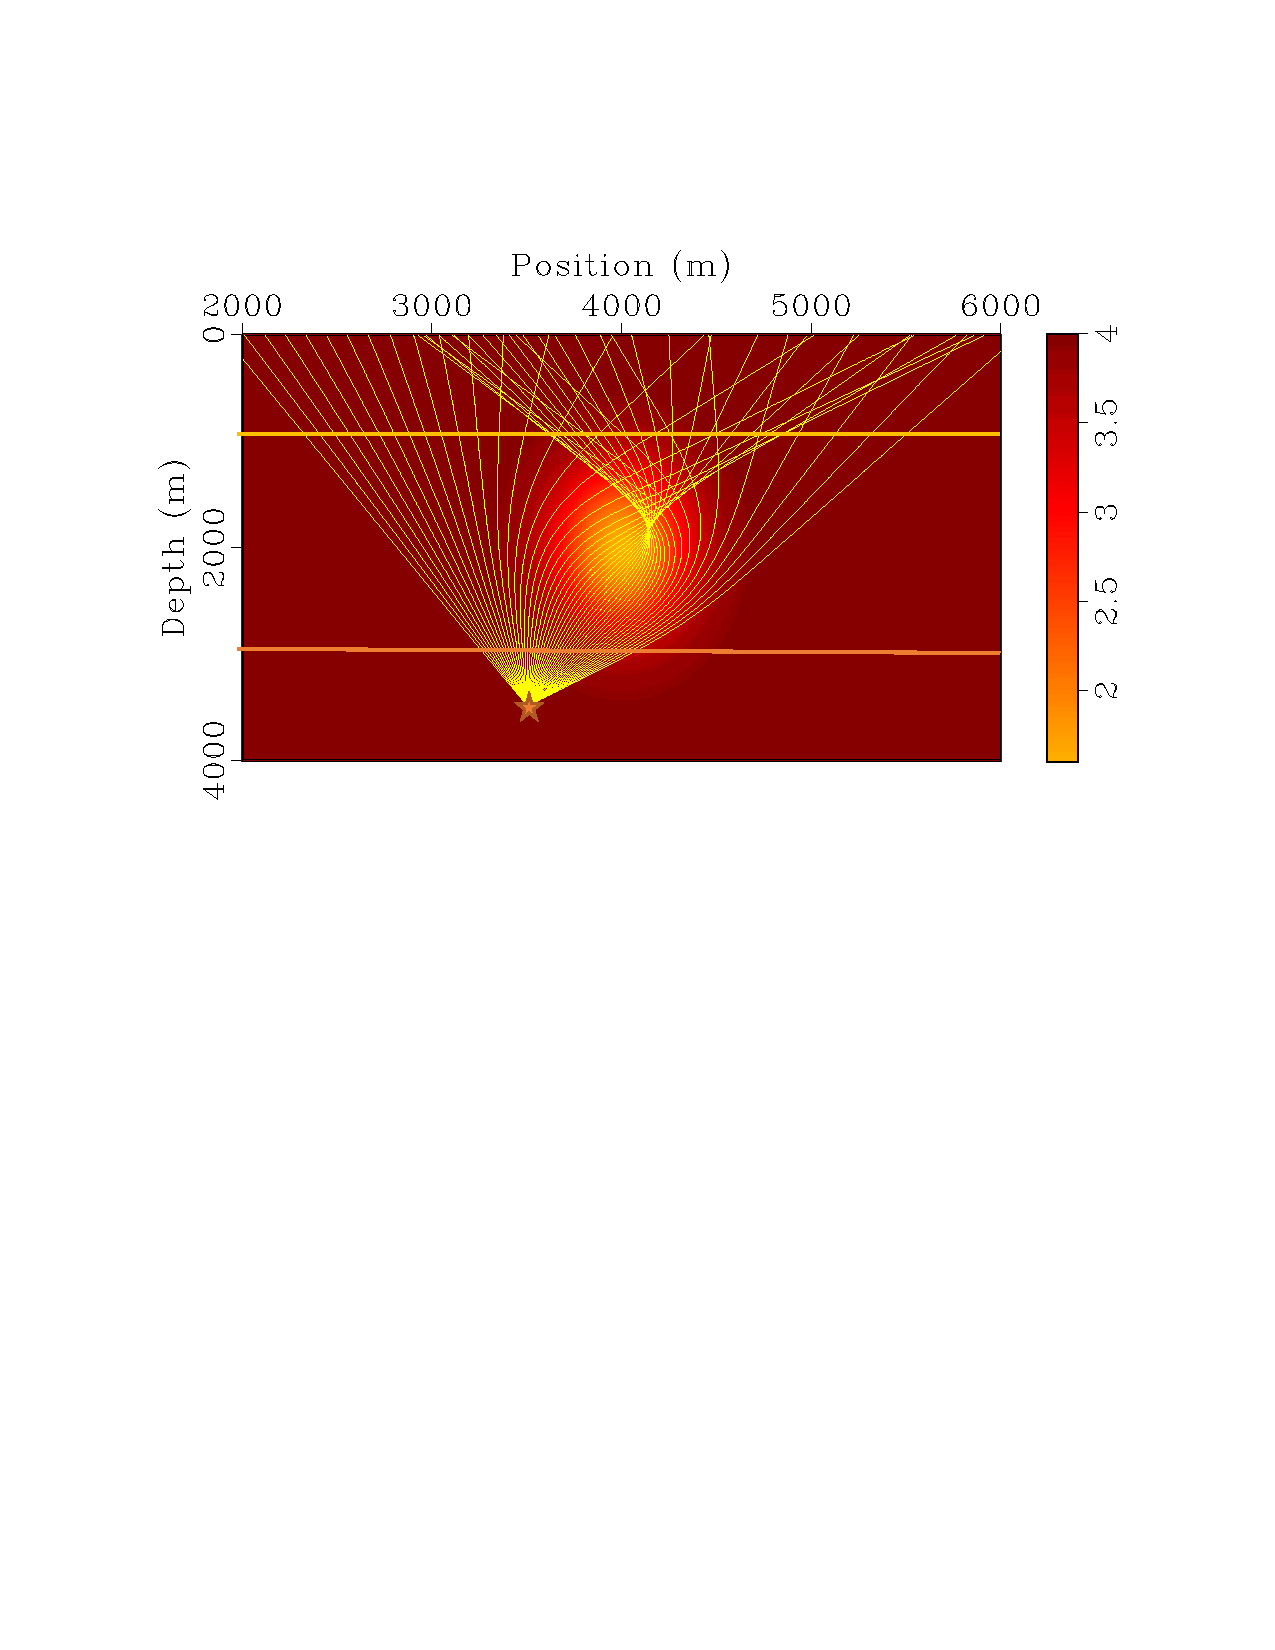
\includegraphics[width=\textwidth]{olensrays0.pdf}
  \caption{Bulk modulus with acoustic lens. Color scale unit is
    GPa. Orange horizontal line is source surface at depth $z_s= 3000$
    m, yellow horizontal
    line is receiver surface at depth $z_r=1000$ m. Point source location for data
    generation at $(3500, 3500)$ m indicated with star. Overlain with rays from point
    source to receiver surface. Outward normal points down at source
    surface, up at receiver surface, so rays are incoming at source
    surface, outgoing at receiver surface.}
  \label{fig:olensrays0}
\end{figure}

%\ref{fig:drecplh0}, \ref{fig:dfwdplh0}
Figure \ref{fig:drecplh0} shows the gather $P_rp_{\rm pt}$, where
$p_{\rm pt}$ is causal field generated by the point source at
$(3500,3500)$ m with a trapezoidal bandpass filter wavelet having
significant energy between 1 and 12.5 Hz. The mute embedded in $P_r$
limits trace positions to 2000 m $ \le x_r \le $ 6000 m, and times to
1.2 s $ \le t \le $ 3 s.

Figure \ref{fig:dhshh0} displays an extended (pressure) source $h_s$, in the form of
traces in the spatial range 2000 m $ \le x_r \le $ 6000 m and time
range 0 s $\le t \le $ 2 s. The modeling operator output $Sh_s$,
obtained from the causal solution $(p, \bv)$ of \ref{eqn:awepm}
with this choice of $h_s$ and $f_s=0,$ by application of the sampling
operator $P_r$ to $p$, is shown in Figure \ref{fig:dfwdplh0}.

\noindent {\bf Remark:} The close resemblance between Figures
\ref{fig:drecplh0} and \ref{fig:dfwdplh0} is not accidental  - the
extended source $h_ s$ shown in Figure \ref{fig:dsrcphh0} is constructed
so that $Sh_s$ (Figure \ref{fig:dfwdplh0}) closely
approximates the point source gather $P_r p_{\rm pt}$ (Figure
\ref{fig:drecplh0}). This construction will be explained in the next section.

\begin{figure}
  \centering
  \subfloat[\label{fig:drecplh0}]{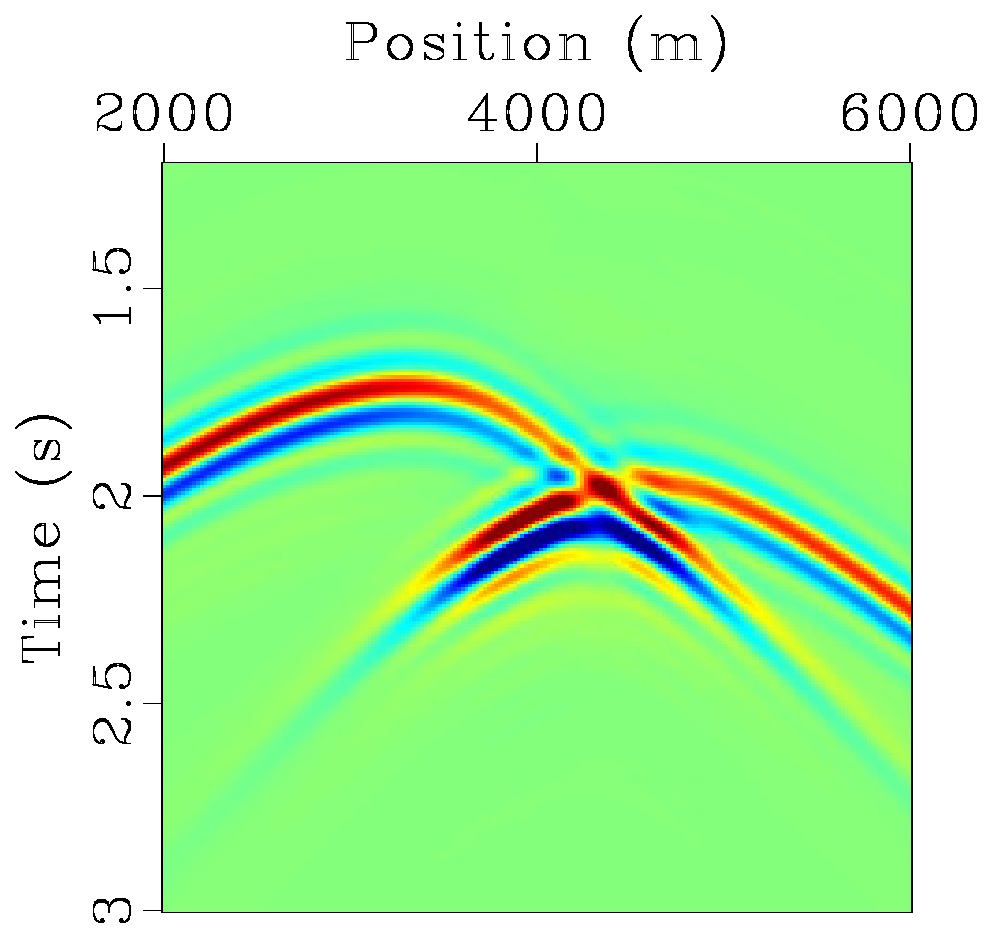
\includegraphics[width=0.32\textwidth]{drecplh0.pdf}}
  \subfloat[\label{fig:dhshh0}]{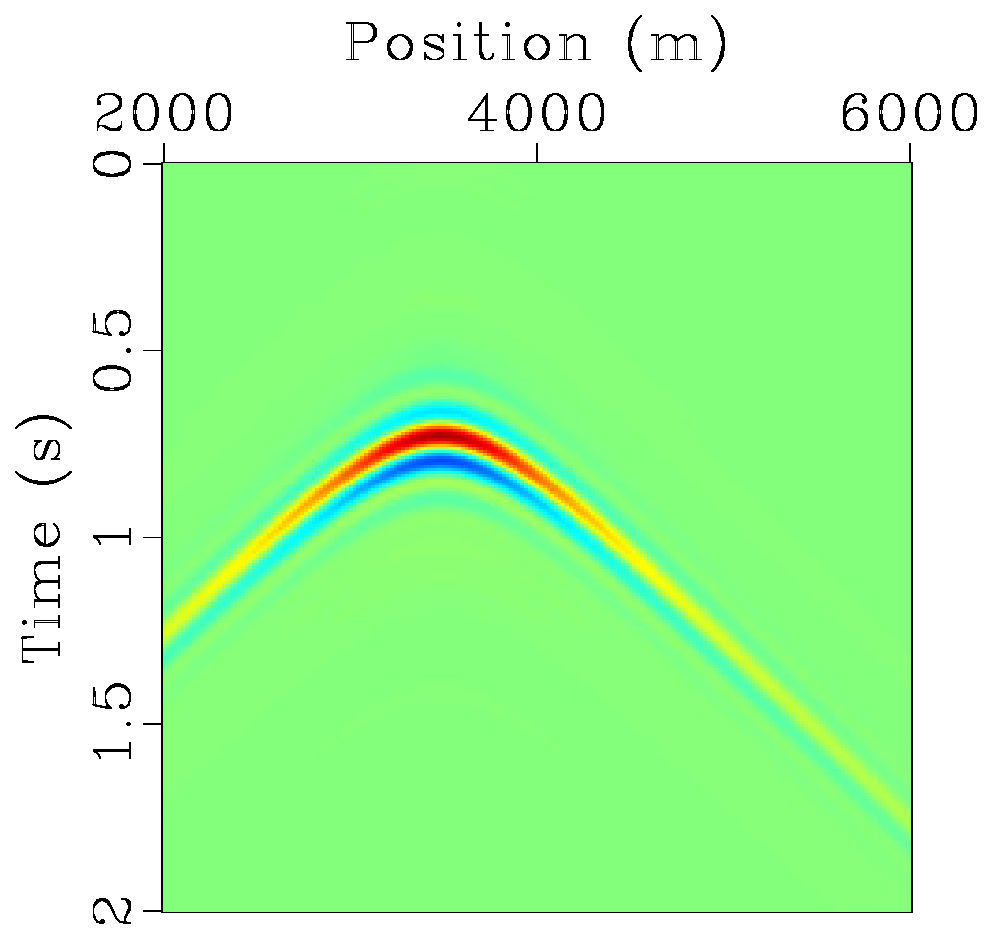
\includegraphics[width=0.32\textwidth]{dhshh0.pdf}}
  \subfloat[\label{fig:dfwdplh0}]{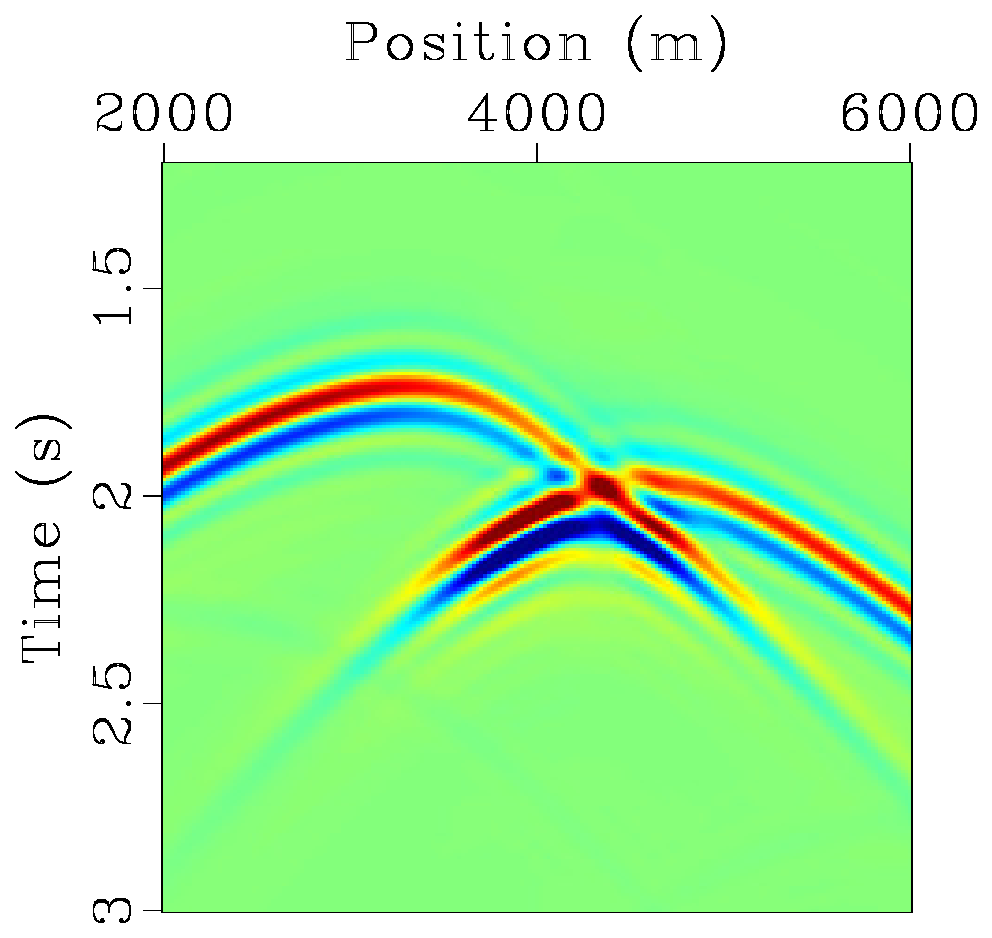
\includegraphics[width=0.32\textwidth]{dfwdplh0.pdf}}
  \caption{Data generated using configuration in Figure
    \ref{fig:olensrays0}. (a) traces from point source at $(3500,3500)$
    with $[1, 2, 7.5, 12.5]$ Hz zero phase trapezoidal bandpass
    filter wavelet, delayed by $0.5$ s. (b) Equivalent extended source on
    the source surface at depth $z_s=3000$ m. (c) Gather generated by
    equivalent source shown in (b). Color scale is same for (a) and (c).}
\end{figure}

The second example is intended as a cartoon of long-offset node
acquisition. It features a depth-dependent increasing
velocity. Figure \ref{fig:ooplrays0} shows bulk modulus field (once again, the
density is constant and $= 1$ g/cm$^3$). The source and receiver
surfaces are horizontal lines, as in the first example, at depths
$z_s=500$ m and $z_r= 100$ m respectively. A point source used to
generate a data traces is positioned at $z_s=500, x_s=10000$ m. The
source wavelet is the same bandpass filter as in
the previous example.

\begin{figure}
  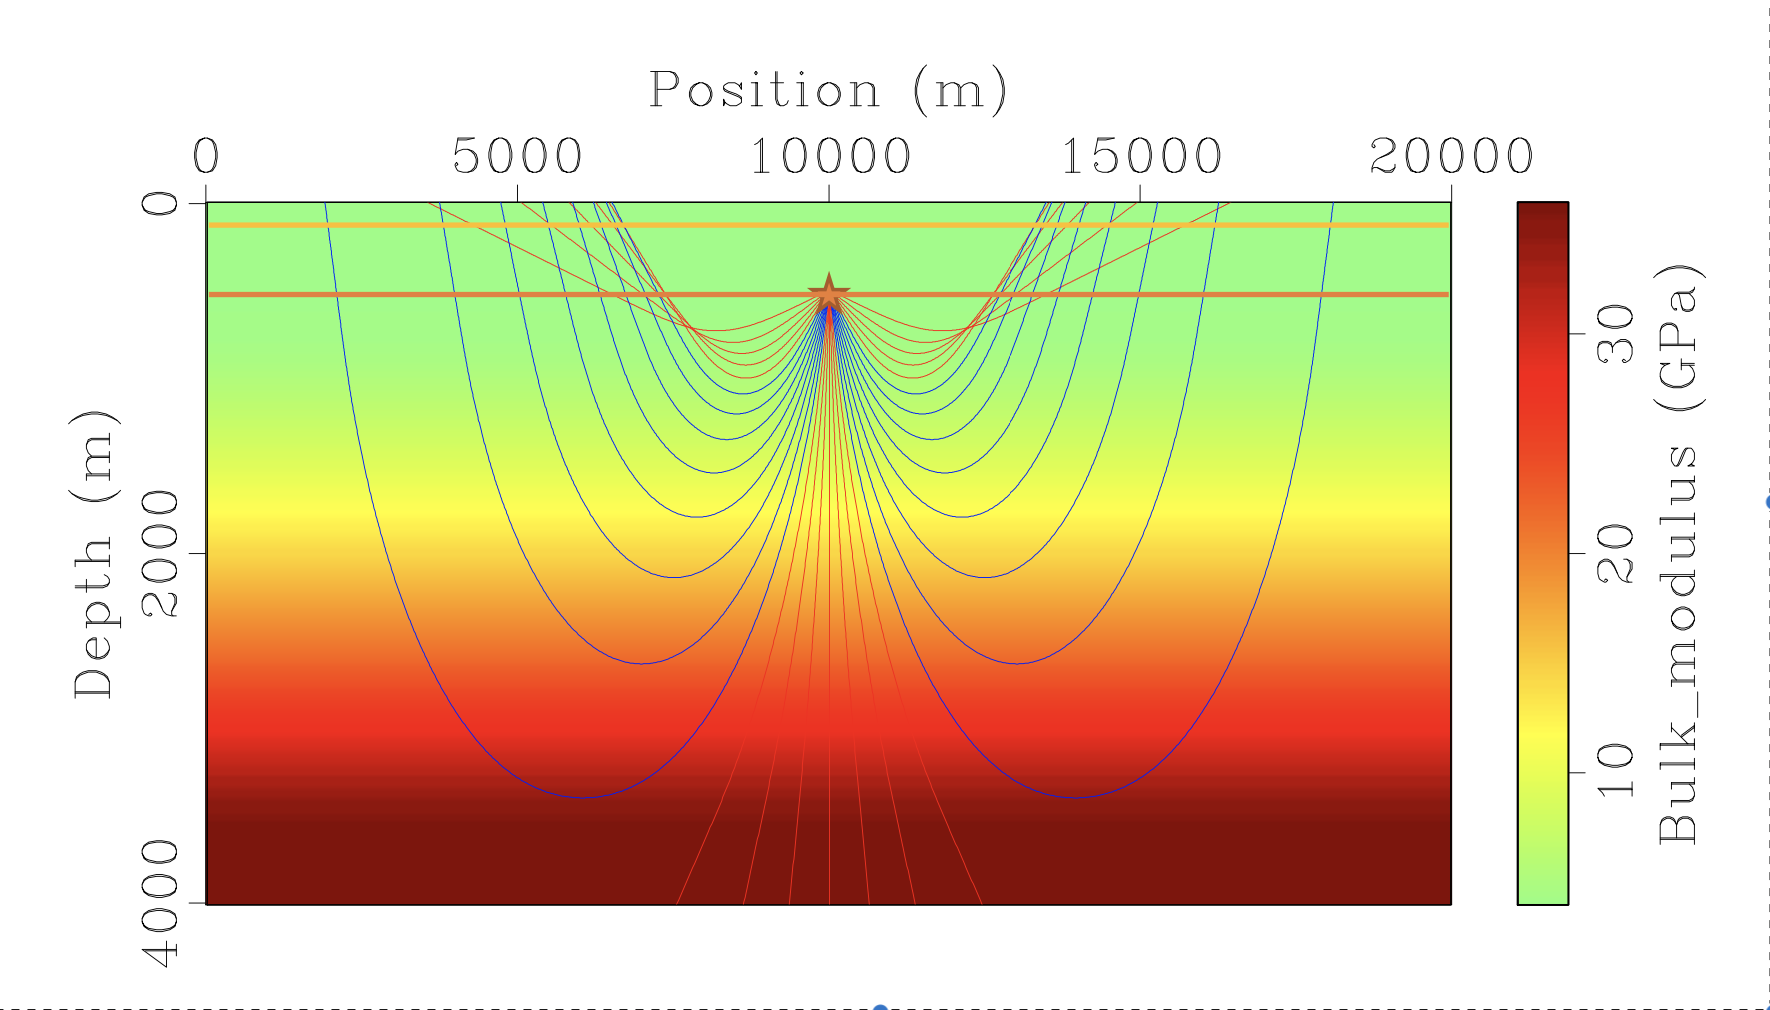
\includegraphics[width=\textwidth]{ooplrays0.png}
  \caption{Bulk modulus generating diving waves. Color scale unit is
    GPa. Orange horizontal line is source surface at depth $z_s= 500$
    m, yellow horizontal
    line is receiver surface at depth $z_r=100$ m. Point source location for data
    generation at $(500, 10000)$ m indicated with star. Overlain with rays from point
    source to receiver surface. Outward normal points up at both source
    and receiver surfaces, so depicted rays are incoming at source
    surface, outgoing at receiver surface. Significance of red
    vs. blue coloring explained in text and caption of Figure \ref{fig:ooxtraysend}.}
  \label{fig:ooplrays0}
\end{figure}

A diving wave arrival is clearly visible in Figure
\ref{fig:ndwraw0}, which displays data traces over the positive offset range $10000 \le
x_r \le 20000$ m. This part of the wavefield is connected to some
refracted rays from the source, those shown in blue in Figure
\ref{fig:ooplrays0}.  Other refracted rays, shown in red in that
Figure, either do not arrive at the receiver surface within the time
range of the data, or are associated with another branch of refracted
arrivals. These two collections of refracted rays result in two
arrival time branches, shown in blue and red in Figure
\ref{fig:ooxtraysend}. The refracted arrival times shown in red,
corresponding to some of the rays shown in red in Figure
\ref{fig:ooplrays0}, corresponds to a refracted arrival that almost
overlaps the direct wave, as is clearly visible in Figure
\ref{fig:ndwraw0}. The arrival combines with the direct wave to result
in an apparent waveform change in the latter. The refracted arrival
times shown in blue in Figure \ref{fig:ooxtraysend} correspond to the
blue rays in Figure \ref{fig:ooplrays0}, and to the faster event
extending to the right of the direct wave.

\begin{figure}
  \centering
  \subfloat[\label{fig:ndwraw0}]{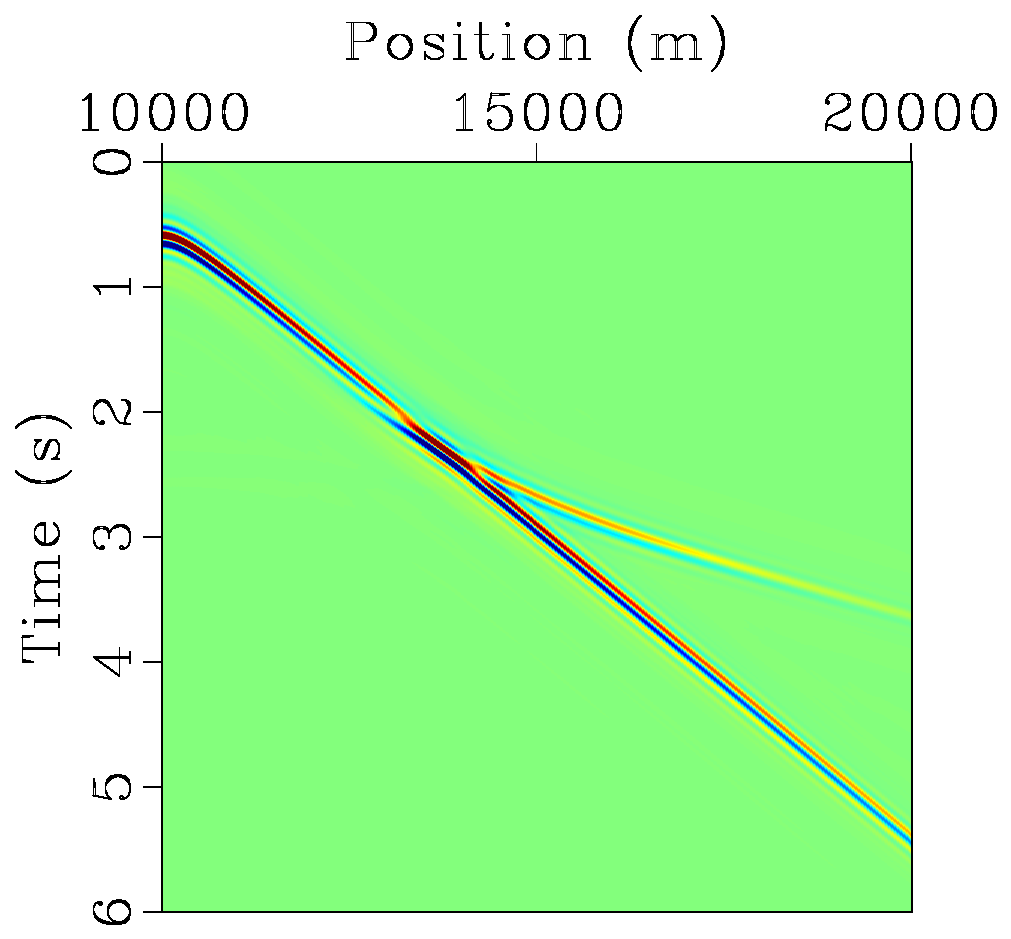
\includegraphics[width=0.4\textwidth]{ndwraw0.pdf}}
  \subfloat[\label{fig:ooxtraysend}]{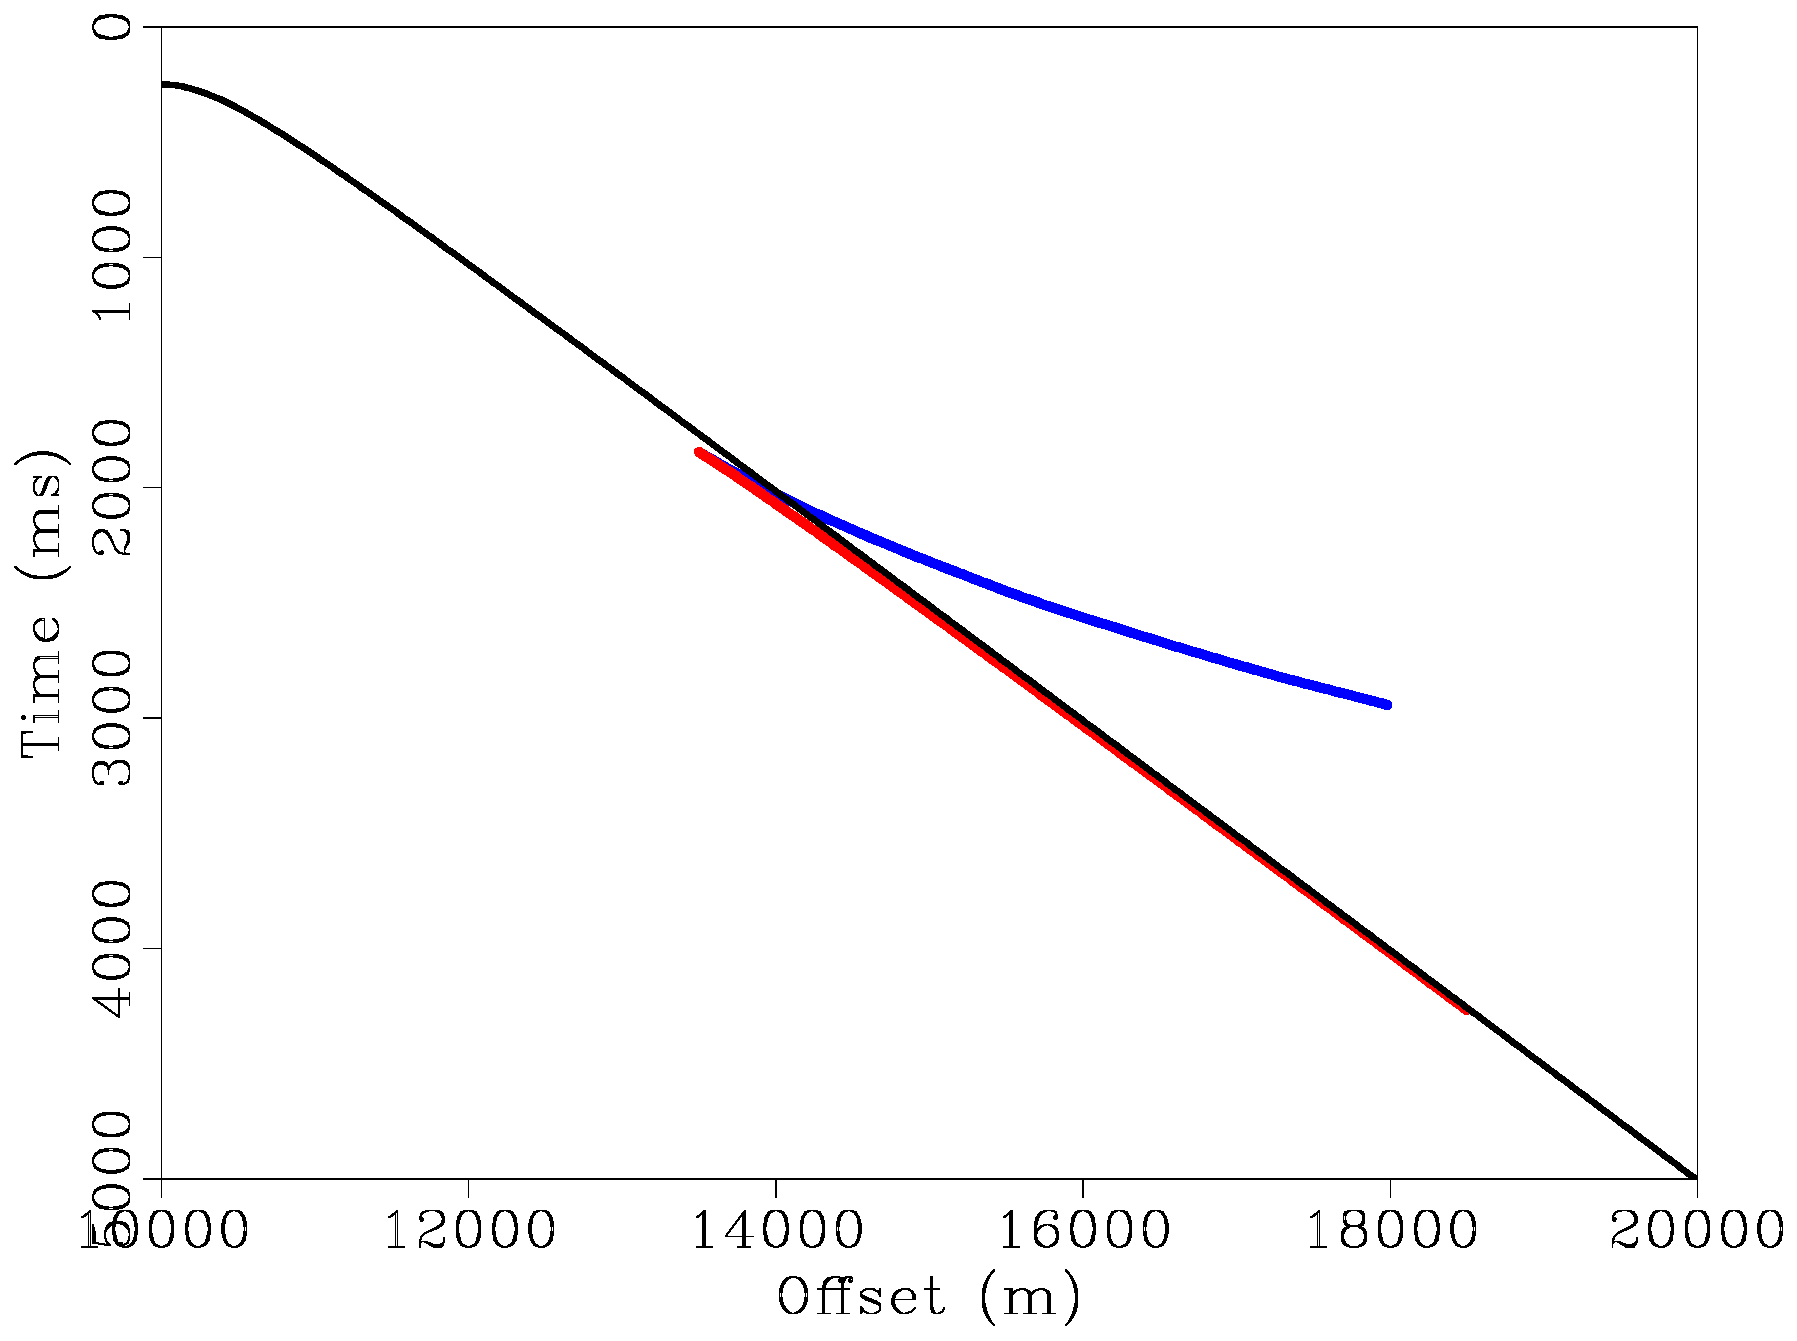
\includegraphics[width=0.4\textwidth]{ooxtraysend.pdf}}
  \caption{Data generated using configuration in Figure
    \ref{fig:ooplrays0}. (a) Traces from point source at $(500,10000)$ m
    with $[1, 2, 7.5, 12.5]$ Hz zero phase trapezoidal bandpass
    filter wavelet, delayed by $0.4$ s. Note that direct arrival
    waveform appears to change where it intersects the diving wave
    arrival visible on the right. (b) Arrival times at surface $z=0$
    of rays leaving source point ($(500,10000)$ m) at $t=0$. Blue
    and red branches corresponds to blue and red rays in Figure
    \ref{fig:ooplrays0}, respectively. The diving wave carried by
    the red rays arrives at the red time branch, which is nearly
    coincident with the direct arrival branch (the black line). This
    part of the refracted wave field combines with
    the direct wave to produce the apparent wavelet change shown in 
    subfigure (a). The blue arrival time branch corresponds to the diving
    wave energy carried by the blue rays in Figure
    \ref{fig:ooplrays0}, displayed in Figure \ref{fig:ndwdata0}.}
\end{figure}

Note that at the source, all of the rays shown in Figure
\ref{fig:ooplrays0} are incoming if the source surface
orientation is chosen with inwards = down, in contrast to the previous
example. The ``blue'' rays, as well as those of the ``red'' rays that
are refracted back towards $z=0$, are outgoing at
the receiver surface if it is oriented so that inwards = down
also.

The ``blue'' arrival can be  isolated via a mute, depicted in Figure
\ref{fig:ndwmute0}.  The
mute includes time truncation at 6 s, and offsets between -10000 and
10000 m. The isolated
diving wave (for positive offsets) is shown in
Figure \ref{fig:ndwdata0}. This muted field can be inverted via the
techniques exploained below, that is, a source field on $z=500$ m
constructed that regenerates approximately the data shown in
\ref{fig:ndwdata0}. In principle the ``red'' arrival, or the ``red''
and ``blue'' arrivals together, could also be inverted by the same
technique, however the ``red'' arrival can only be isolated by
subtraction of the direct wave, which is not itself incoming (or
outgoing). In this paper, the simpler option is pursued, of inverting
the muted diving wave arrival in Figure \ref{fig:ndwdata0}, in order
to illustrated the localization mechanism at the heart of the inversion.

\begin{figure}
  \centering
  \subfloat[\label{fig:ndwmute0}]{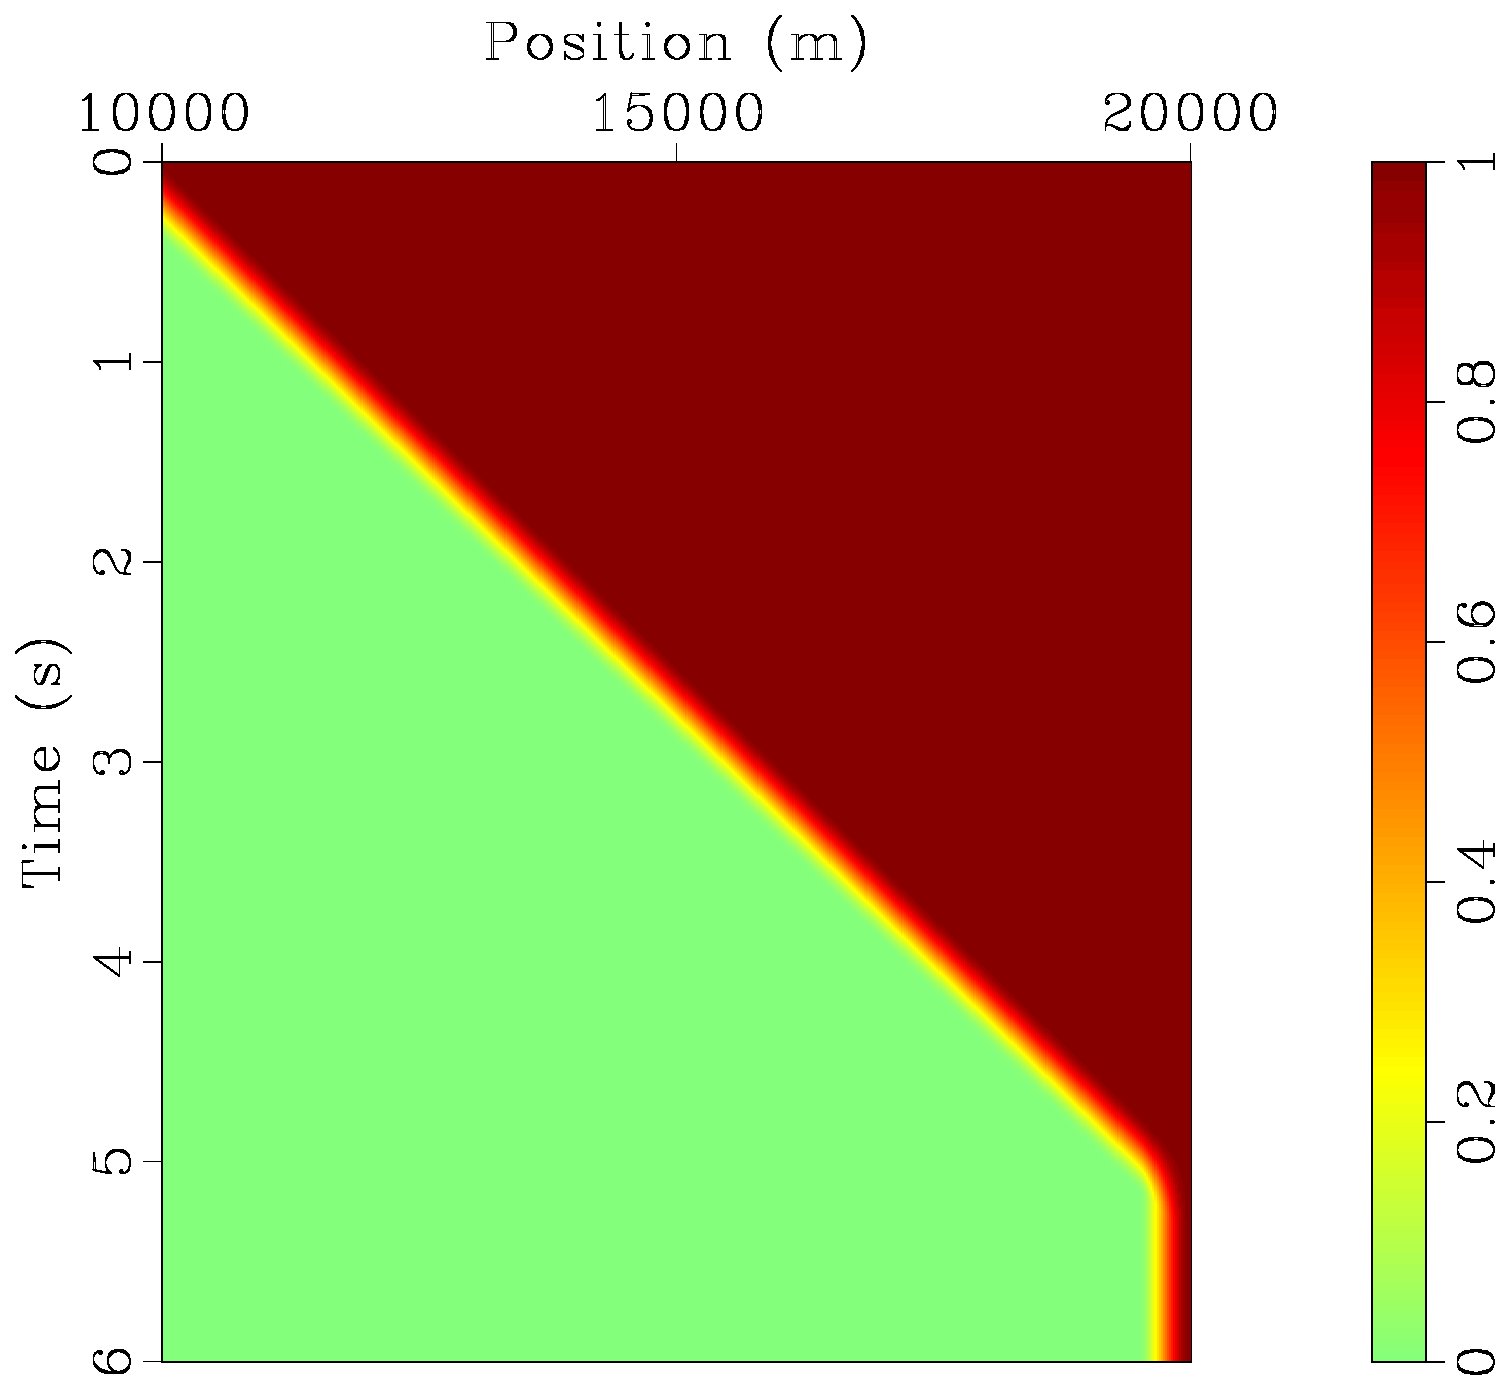
\includegraphics[width=0.4\textwidth]{ndwmute0.pdf}}
  \subfloat[\label{fig:ndwdata0}]{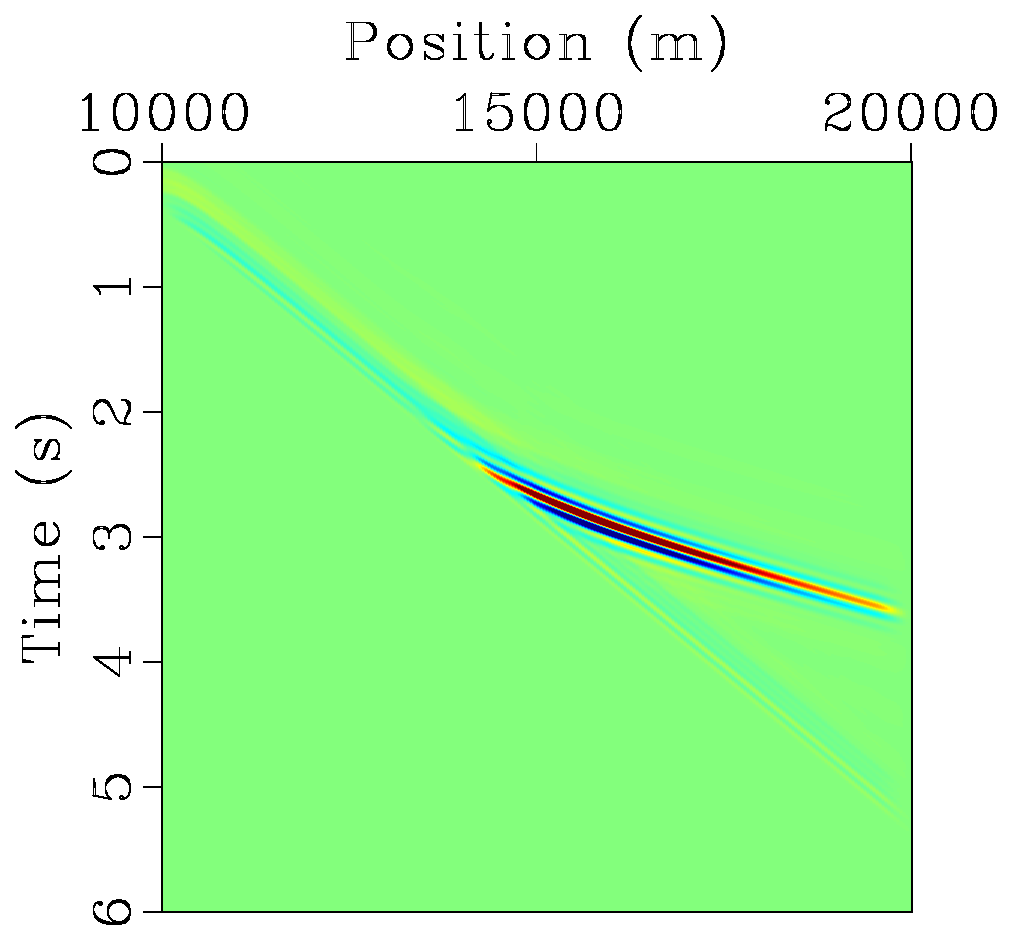
\includegraphics[width=0.4\textwidth]{ndwdata0.pdf}}
  \caption{(a) Mute function,
    incorporated in the sampling operator $P_r$, designed to isolate
    the diving wave branch visible in Figure \ref{fig:ndwraw0}. (b) Diving wave
    gather, mute in (a) applied to data in Figure
    \ref{fig:ndwraw0}. Color scale is 5 tmies that of Figure \ref{fig:ndwraw0}.}
\end{figure}

\section{Time Reversal}

There is no measurement surface surrounding the region of propagation
in the surface source inversion problem. Therefore the time reversal
construction, as found in the literature on photoacoustic tomography,
must be localized in space-time, so that an artificial surrounding
region may be constructed. It must also be modified to produce a
source, rather than a slice of the pressure field. The assumption of
incoming rays at the source surface and outgoing rays at the receiver
surface makes both modifications possible.

The construction takes place in three stages: first, an acoustic field
with high-frequency energy propagating along an incoming ray family is
identified as the causal solution of an inhomogeneous boundary value
problem {\em locally and on the inside}. The boundary value is simply
the restriction of the pressure field to the surface. Second, the same
causal solution is identified as the causal solution of an acoustic
problem with source, singular on the surface in the fashion of
equation \ref{eqn:awepm}. The source amplitude is proportional to the
velocity field sampled on the surface. Third, this identification is
used twice, first to propagate the receiver data backwards in time as
the solution of an anti-causal problem with source on the receiver
surface; the velocity field of which is sampled on the source surface;
then the causal problem is solved with the source built from the
velocity samples. This solution must asymptotically approximate the
field generating the data, along the ray fields carrying all of the
high-frequency energy. Therefore the reconstructed source is an
approximate solution of the problem \ref{eqn:esis} for $\alpha=0$.

%For the bulk of this section, the source and receiver surfaces are
%arbitrary smooth surfaces, as there is no conceptual penalty in
%dropping the assumption that they are coordinate surfaces.

\subsection{Field localization}
The first task is to view an acoustic field locally as a solution of a
boundary value problem with prescribed pressure on the boundary of a
domain, as is the case in the photoacoustic tomography configuration.

In this subsection $(p,\bv)$ is a solution of the homogeneous acoustic system
\begin{eqnarray}
\label{eqn:awefree}
  \frac{1}{\kappa}\frac{\partial p}{\partial t} & = & - \nabla \cdot \bv, \nonumber \\
  \rho\frac{\partial \bv}{\partial t} & = & - \nabla p,
\end{eqnarray}
The source surface $\Sigma$ is given a choice of unit normal field ${\bf
  n}$. Rays carrying
high-frequency energy in $(p,\bv)$ pass through $\Sigma$, and
intersect $\Sigma$ only at times
$>0$. Also, the velocity
vectors of all such rays have a negative ${\bf n}$ component where
they cross $\Sigma$. Construct a time interval $[0,\tau]$ and
a region in space $\Omega^+$ containing $\Sigma$ so that $\Sigma$ forms
part of the boundary $\partial \Omega^+$ of $\Omega^+$, ${\bf n}$ is the
outward unit normal to $\Omega^+$ on $\Sigma$, and the energetic
rays cross $\partial \Omega^+$ {\em only} at
points of $\Sigma$ in the time interval $[0,\tau]$ - that is, in time
less than $\tau$ the rays do not reach other parts of $\partial
\Omega^+$. Note that the rays are {\em incoming} to $\Omega^+$ in the terminology
introduced earlier. See Figure \ref{fig:omegarays}.

\begin{figure}
  \centering
  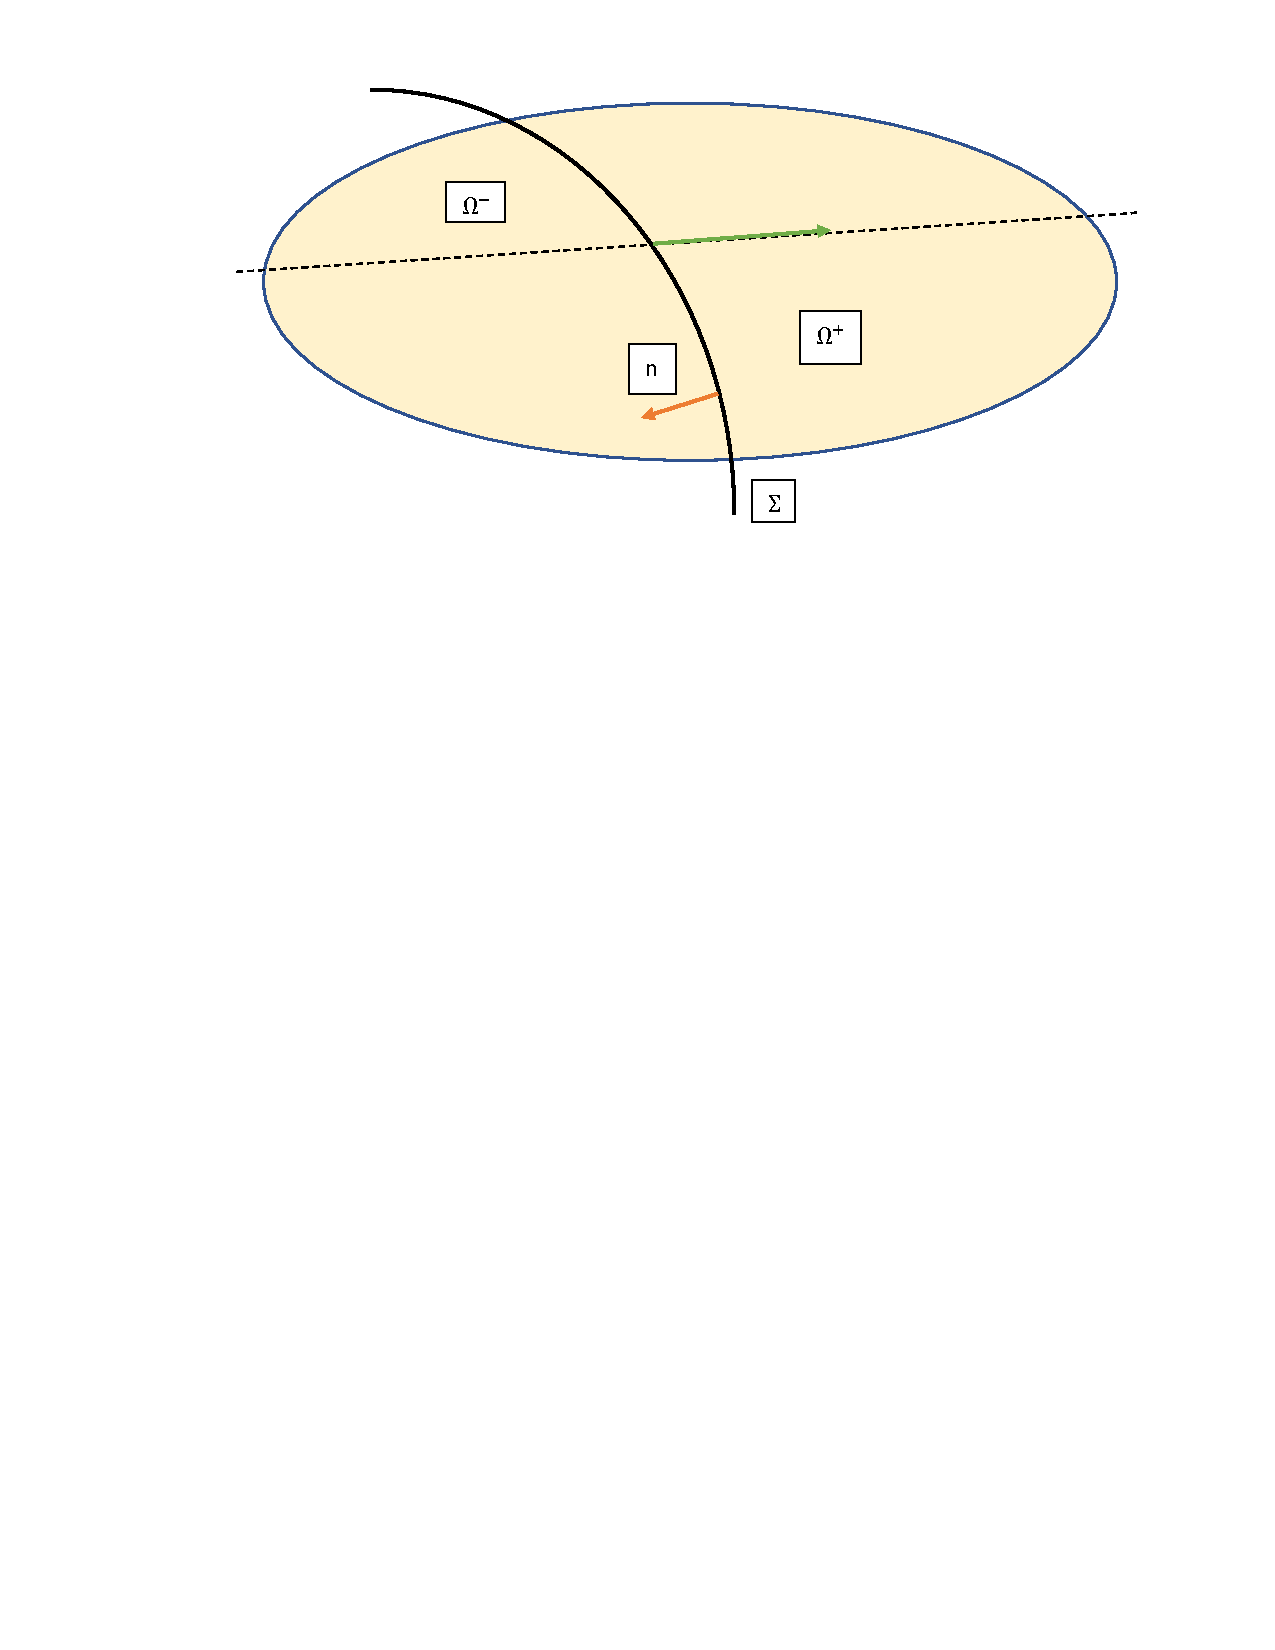
\includegraphics[width=0.8\textwidth]{omegarays.pdf}
  \caption{Localization near crossing points of rays. $\Sigma$ is
    source surface.  Dashed line is part of a ray carrying high
    frequency energy. Ray velocity vector has negative component in
    direction of unit normal ${\bf n}$ (outward, in chosen
    orientation). $\Omega^+$ contains all ray segments for times
    $0 \le t \le \tau$ (green arrow). Rays intersect boundary
    $\partial \Omega^+$ only in $\Sigma$ for this time
    range. $\Omega^-$ lies on outward side of $\Sigma$, which is part
    of its boundary. The domain $\Omega$ is the union of $\Omega^+$
    and $\Omega^-$.}
  \label{fig:omegarays}
\end{figure}

Consequent to this ray geometry, conclude that the field $(p,\bv)$  is asymptotically negligible both
throughout $\Omega^+$ at $t=0$ and at all points of 
$\partial \Omega^+$ except for $\Sigma$, for $0\le t \le \tau$. So $(p,\bv)$ differs
negligibly from the solution of the boundary value problem 
\begin{eqnarray}
\label{eqn:aweloc}
  \frac{1}{\kappa}\frac{\partial \tilde{p}}{\partial t} & = & - \nabla \cdot \tilde{\bv}, \nonumber \\
  \rho\frac{\partial \tilde{\bv}}{\partial t} & = & - \nabla
                                                    \tilde{p}, \nonumber \\
  \tilde{p}(\bx,t) & = & p(\bx,t) \mbox{ for } \bx \in \Sigma, 0 \le t \le 
  \tau, \nonumber \\
  \tilde{p}(\bx,t) & = & 0 \mbox{ for } \bx \in \partial \Omega^+ \setminus \Sigma, 0 \le t \le
 \tau.
\end{eqnarray}

\subsection{Source representation}

The fields involved in the surface source extension are causal and
source-generated, rather than solutions of boundary value problems
such as the system \ref{eqn:aweloc}. To transition to a source
representation, begin by extending the domain $\Omega^+$, lying on the
incoming side of the surface $\Sigma$, to a full neighborhood $\Omega$
of $\Sigma$
by adding a domain $\Omega^-$ on the outside (see Figure
\ref{fig:omegarays}). Once again, construct $\Omega^-$ so that none of
the rays carrying high-frequency energy cross the boundary of
$\Omega^-$ except at $\Sigma$. Extend the field $(\tilde{p},\tilde{\bv})$ to the
full neigborhood $\Omega$ by solving the system \ref{eqn:aweloc} with
$\Omega^+$ replaced by $\Omega^-$. Thus the extended
field is pieced together out of causal fields solving the boundary value
problem on either side of the boudary, with {\em the same} boundary
condition, that is, the trace of $p$ on $\Sigma$. Thus the extended
field is continuous in $p$. it is not however continuous in
$\bv$, as will be seen shortly. More precisely, the normal component
$\bv\cdot {\bf n}$
has a discontinuity, while the tangential components are continuous.
The jump in
$\bv\cdot {\bf n}$ contributes a delta function to the gradient: as a
field in the whole neigborhood $\Omega$, $(\tilde{p},\tilde{\bv})$
solves
\begin{eqnarray}
\label{eqn:awebase}
  \frac{1}{\kappa}\frac{\partial \tilde{p}}{\partial t} & = & [\bv \cdot {\bf n}]_{\Sigma}\delta_{\Sigma}
                                                      - \nabla \cdot \tilde{\bv}, \nonumber \\
  \rho\frac{\partial \tilde{\bv}}{\partial t} & = & - \nabla \tilde{p}, \nonumber \\
  \tilde{p}(\bx,t) & = & 0 \mbox{ for } \bx \in \partial \Omega, 0 \le t \le 
  \tau, \nonumber \\
  \tilde{p} & = & 0 \mbox{ for } \bx \in \Omega^+, t , \nonumber \\
  \tilde{\bv} & = & {\bf 0} \mbox{ for } \bx \in \Omega^+, t = 0.       
\end{eqnarray}
The square bracket denotes the jump in the quantity enclosed across
$\Sigma$, from the outside to the inside. Since ${\bf n}$ points from
the inside to the outside, this convention contributes another minus
sign.

This representation is even better than it looks: since the ray
families in $\Omega^{\pm}$ cross the boundary only at $\Sigma$ within
the prescribed time interval, the
solution changes only by an asymptotically negligible amount in
$\Omega$ for $0 \le t \le \tau$ if the boundary condition is removed
and the system is solved for all of space-time.

There is a downside, namely the apparent necessity of constructing the
solution in $\Omega^-$ so that the jump of $\bv \cdot {\bf n}$ may be
computed. That is actually not necessary, however.
This is best seen by analyzing a generic geometric optics
component associated to the phase function $\psi$ in $\Omega^+$ and its family of
rays. The acoustic field is assembled by a sum (in the continuum, an
integral) over such solutions. A particular summand looks like
\begin{equation}
  \label{eqn:go}
   a(\bx,t)e^{i\omega (t - \psi(\bx))}.
\end{equation}
for $\bx \in \Omega^+$.
The phase $\psi$ solves the eikonal equation, the amplitude $a$ the
related transport equation. The restriction of $p$
to $\Sigma$ determines $\psi$ (and $a$) restricted to $\Sigma$, essentially by
Fourier synthesis. Since the eikonal
equation is even in $\nabla \psi$,  and $\psi$ restricted to $\Sigma$
determines the tangential derivatives of $\psi$, the normal component
of $\nabla \psi$ is determined up to sign by the boundary values of
$p$. The spatial component of a ray $X(t)$ associated to $\psi$ solves
the ordinary differential equation
\begin{equation}
  \label{eqn:ray}
  \frac{dX}{dt} = \nabla \psi(X).
\end{equation}
The normal component of this ray must be negative (in
$\Omega^+$) - this is the incoming condition, and guarantees that the
ray does not intersect $t=0$ in $\Omega^+$ near $\Sigma$, justifying the initial
condition in \ref{eqn:aweloc}. Similarly, the normal component must be
positive in $\Omega^-$ near $\Sigma$. But both must have the same magnitude, since
$\psi$ solves the eikonal equation - so they are negatives of each
other. For causal solutions such as $(\tilde{p},\tilde{\bv})$, the
Newton's law equation in \ref{eqn:aweloc} is equivalent to
\begin{equation}\label{eqn:newt}
  \tilde{\bv}(\bx,t) = -\frac{1}{\rho}\int_{-\infty}^t ds \nabla \tilde{p}(\bx,s),
\end{equation}
except at $\Sigma$.
it follows that the normal components of $\tilde{\bv}$ have limits at
point of $\Sigma$ 
that are opposite in sign: for $\bx \in \Sigma$,
\[
  \lim_{\zeta \rightarrow 0} (\tilde{\bv}(\bx+\zeta {\bf n}(\bx),t) \cdot {\bf
    n}(\bx)) = 
-\lim_{\zeta \rightarrow 0} (\tilde{\bv}(\bx-\zeta {\bf n}(\bx),t) \cdot {\bf
  n}(\bx))
\]
whence
\begin{equation}
   \label{eqn:vjump}
   [\tilde{\bv} \cdot {\bf n}] = 2 \lim_{\zeta
  \rightarrow 0} (\tilde{\bv}(\bx -\zeta {\bf
  n}(\bx),t) \cdot {\bf n}(\bx))
\approx 2 \bv(\bx) \cdot {\bf n}(\bx)
\end{equation}
That is, at least over the short time interval $0 \le t \le \tau$,
$(p,\bv)$ is asymptotically approximated in $\Omega^+$ by
$(\tilde{p},\tilde{\bv})$, which solves
\begin{eqnarray}
\label{eqn:awesrc}
  \frac{1}{\kappa}\frac{\partial\tilde{p}}{\partial t} & = & h \delta_{\Sigma}
                                                      - \nabla \cdot \tilde{\bv}, \nonumber \\
  \rho\frac{\partial \tilde{\bv}}{\partial t} & = & - \nabla \tilde{p}, \nonumber \\
  \tilde{p} & = & 0 \mbox{ for } \bx \in \Omega, t=0, \nonumber \\
  \tilde{\bv} & = & {\bf 0} \mbox{ for } \bx \in \Omega, t = 0.       
\end{eqnarray}
with $h = 2 \bv \cdot {\bf n}$ on $\Sigma$.

This result appears limited by the short time assumption (on $\tau$)
and the corresponding spatial localization to $\Omega^+$. However
neither of these apparent limitations is real. The short time
assumption may be relaxed by windowing the fields to short time
windows then adding up the results. The approximating fields
$(\tilde{p}, \tilde{\bv})$ are themselves approximated by ray
theory solutions. The assumptions on rays crossing source and receiver
surfaces are global, and extend the approximation \ref{eqn:awesrc}
globally. Thus the last two conditions may be replaced by the basic
causality condition
\begin{eqnarray}
  \label{eqn:awesrcmod}
  \frac{1}{\kappa}\frac{\partial\tilde{p}}{\partial t} & = & h \delta_{\Sigma}
                                                      - \nabla \cdot \tilde{\bv}, \nonumber \\
  \rho\frac{\partial \tilde{\bv}}{\partial t} & = & - \nabla \tilde{p}, \nonumber \\
  \tilde{p} & = & 0 \mbox{ for }  t \ll 0, \nonumber \\
  \tilde{\bv} & = & {\bf 0} \mbox{ for } t \ll 0.       
\end{eqnarray}
The effect of this change on the receiver surface traces of $\tilde{p}$ and
$\tilde{\bv}$ is negligible.

An example has already appeared in Figure \ref{fig:dhshh0}. In this
example, the field $(p, \bv)$ is the point source solution with the
point source depicted in Figure \ref{fig:olensrays0}, located at
$(3500, 3500)$ m. The role of $\Sigma$ is played by the source surface $\Sigma_s=
\{z=z_s=3000 \mbox{ m}\}$, and near this surface the field solves the source-free
system \ref{eqn:awefree}. The ``inside'' in this example is the region
$z > z_s$, and the outward unit normal is therefore ${\bf n}=(0,0,-1)^T$.
Thus $(p,\bv)$ should be asymptotically close to the solution
$(\tilde{p},\tilde{\bv})$ of the
system \ref{eqn:awesrc} in the region $z< z_s$, at least at locations
connected by the ray field shown in Figure \ref{fig:olensrays0} to the
source surface, provided that the source amplitude $h$ is chosen $=
-2v_z$ on $\Sigma_s=\{z=z_s\}$. Figure \ref{fig:dhshh0} displays exactly this $h$, and
\ref{fig:dfwdplh0} the traces of $\tilde{p}$ on the
  receiver surface $z=z_r=1000$ m, which satisfies the ray condition. The extremely
close match between Figures \ref{fig:drecplh0} (traces of $p$ on $\Sigma_r$) and
\ref{fig:dfwdplh0} is consistent with the conclusion reached here.

\subsection{Approximate Inversion}

The time-reversal construction can now be translated into the context
of seismic surface source inversion. Assume that $(p,\bv)$ is a
solution of the free-space acoustic system \ref{eqn:awefree}, with
high-frequency energy carried by a ray family that satisfies the
criteria described earlier: incoming at the source surface $\Sigma_s$
with normal field ${\bf n}_s$, outging at the receiver surface
$\Sigma_r$ with normal field ${\bf n}_r$, and every ray crossing
$\Sigma_r$ meets $\Sigma_s$. The goal of this subsection is to
describe a procedure that constructs a source field $h_s$ on
$\Sigma_s$ so that $Sh_s \approx P_rp$, thus approximately inverting
the modeling operator $S$.

The sampled fields $(P_rp,P_r\bv)$ on $\Sigma_r$
is negligible for large $t$. Due the outgoing assumption,
$(p,\bv)$ are negligible for large $t$ near $\Sigma_r$. The
integrated Newton's law \ref{eqn:newt} acquires a minus sign if the
integration from $-\infty$ to $t$ is replaced by integration from $t$
to $\infty$. Apply the construction of the last subsection in reverse
time, to conclude
that $(p,\bv)$ is approximated by $(\hat{p},\hat{\bv})$, where the
latter solves the time-reversed problem
\begin{eqnarray}
\label{eqn:awerecglob}
  \frac{1}{\kappa}\frac{\partial\hat{p}}{\partial t} & = & h_r \delta_{\Sigma_r}
                                                      - \nabla \cdot \hat{\bv}, \nonumber \\
  \rho\frac{\partial \hat{\bv}}{\partial t} & = & - \nabla \hat{p}, \nonumber \\
  \hat{p} & = & 0 \mbox{ for } t\gg 0, \nonumber \\
  \hat{\bv} & = & {\bf 0} \mbox{ for } t \gg 0.       
\end{eqnarray}
with $h_r = -2P_r(\bv \cdot {\bf n}_r)$.

By construction, high-frequency energy in $(\hat{p},\hat{\bv})$ is
carried by the same ray family as for $(p,\bv)$. Every ray passes over
$\Sigma_s$ and is incoming there. Since $(p,\bv)$ vanishes for $t \ll
0$ near $\Sigma_s$, $(\hat{p},\hat{\bv})$ is negligible there,  So
the construction detailed in the last two sections is applicable
again, and the reverse-time field $(\hat{p},\hat{\bv})$ is
approximated by the forward-time field $(\tilde{p},\tilde{\bv})$ that solves
\begin{eqnarray}
\label{eqn:awesrcglob}
  \frac{1}{\kappa}\frac{\partial\tilde{p}}{\partial t} & = & h_s \delta_{\Sigma_s}
                                                      - \nabla \cdot \tilde{\bv}, \nonumber \\
  \rho\frac{\partial \tilde{\bv}}{\partial t} & = & - \nabla \tilde{p}, \nonumber \\
  \tilde{p} & = & 0 \mbox{ for } t\ll 0, \nonumber \\
  \tilde{\bv} & = & {\bf 0} \mbox{ for } t \ll 0.       
\end{eqnarray}
with $h_s = 2P_s(\hat{\bv} \cdot {\bf n}_r) \approx 2P_s(\bv \cdot
{\bf n}_r)$.

\subsection{Summary}
The surface source version of the time reversal construction involves three steps: given
pressure data $P_rp$ on the receiver surface $\Sigma_r$ for a solution
$(p,\bv)$ of the system \ref{eqn:awefree} satisfying the ray conditions,
\begin{itemize}
\item[1. ] create a source $h_r$ on $\Sigma_r$
  by multiplying the corresponding normal velocity trace by $-2$: $h_r = -2P_r(\bv
  \cdot {\bf n}_r)$;
\item[2. ] propagate $h_r$ backwards in time by solving the system
  \ref{eqn:awerecglob} for the acoustic field $(\hat{p},\hat{\bv})$;
\item[3. ] create a source $h_s$ on $\Sigma_s$ by  multiplying tne
  normal velocity trace of $\hat{\bv}\cdot {\bf n}_s$ by 2: $h_s = 2P_s(\hat{\bv}
  \cdot {\bf n}_s)$.
\end{itemize}
Then $P_r p \approx Sh_s$.

The surface source representation part of the construction shows that
under the assumed ray conditions, a solution of \ref{eqn:awefree} is
asymptotically the same near the receiver surface $\Sigma_r$ as the
solution of the system \ref{eqn:awepm} with a suitable source
$h_s$ (and zero velocity source, $f_s=0$). Therefore this
construction also inverts the modeling operator $S$ in the sense that
$Sh_s\approx S\tilde{h_s}$ if $P_rp \approx S\tilde{h_s}$. That is,
this construction produces an asymptotic right inverse of $S$: it
does not necessily (approximately) recover the source that generates
the data, but recovers some source that generates the data.

\subsection{Example: Lens}
The first example uses the acoustic lens model (Figure
\ref{fig:olensrays0}), with $\Sigma_s$ = horizontal line at depth 
3000 m, and $\Sigma_r$ = horizontal line at depth 1000 m. The pressure
data to be inverted is the sampling of the pressure field on
$\Sigma_r$, generated by the point source shown in the figure, at
$(3500, 3500)$ m (Figure \ref{fig:drecplh0}). However, I will invert
this data in a homogeneous medium with $\kappa \equiv 4$ GPa. This
choice illustrates two facts about surface source inversion and
approximate inversion based on time reversal. First, the success of the inversion demonstrates the
insensitivity of the time reversal method to ray multipathing
(triplication), evident in the data (Figure \ref{fig:drecplh0}).
%s respectively
Second, it is entirely possible to invert data in a material model
other than the one in which it was produced (in the case of synthetic
data, of course). This
capability is critically important in the application of 
approximate source inversion in nonlinear extended inversion, where the early iterations
involve solution of the source estimation problem \ref{eqn:esis} at
(possibly very) wrong material models ${\bf c}$. Successful extension
methods maintain data fit throughout the course of the inversion.
%The source time dependence is again a [1, 2.5,
%10, 12.5] Hz trapezoidal bandpass filter.

As noted earlier (and visible in Figure \ref{fig:olensrays0}), the acoustic field in this example satisfies the ray
conditions on which the time reversal construction is based: The rays
are incoming at $\Sigma_s$, outgoing at $\Sigma_r$ and all rays
carrying significant energy at points of $\Sigma_r$ pass over
$\Sigma_s$. The outward unit normal at $\Sigma_s$ is ${\bf n}_s ={\bf
  e}_z=(0,1)$; at $\Sigma_r$, it's ${\bf n}_r =-{\bf
  e}_z=(0,-1)$. So the source on the receiver surface $\Sigma_r$, input to reverse time propagation
(system \ref{eqn:awerecglob}, generating the fields $(\hat{p},\hat{\bv})$) is
$h_r=2P_rv_z$ (the field $P_rv_z$ is depicted in Figure \ref{fig:dfwdvzlh0}). After reverse time propagation , the approximate
inversion $\hat{h}_s=2P_s\hat{v}_z$ is shown in Figure
\ref{fig:dinvhslh0}. It differs considerably from the source field used to
generate the data (Figure \ref{fig:dsrcphh0}), however when used as the
source in forward modeling (system \ref{eqn:awesrcglob}) {\em with the
  same material parameters used in the inversion}, it generates a
pressure gather on $\Sigma_r$ (Figure \ref{fig:drerecplh0}) very
closely 
approximating the input gather (Figure \ref{fig:dfwdplh0}). The
difference is plotted on the same color scale in Figure
\ref{fig:ddiffrecplh0}.

\begin{figure}
  \centering
  \subfloat[\label{fig:dfwdvzlh0}]{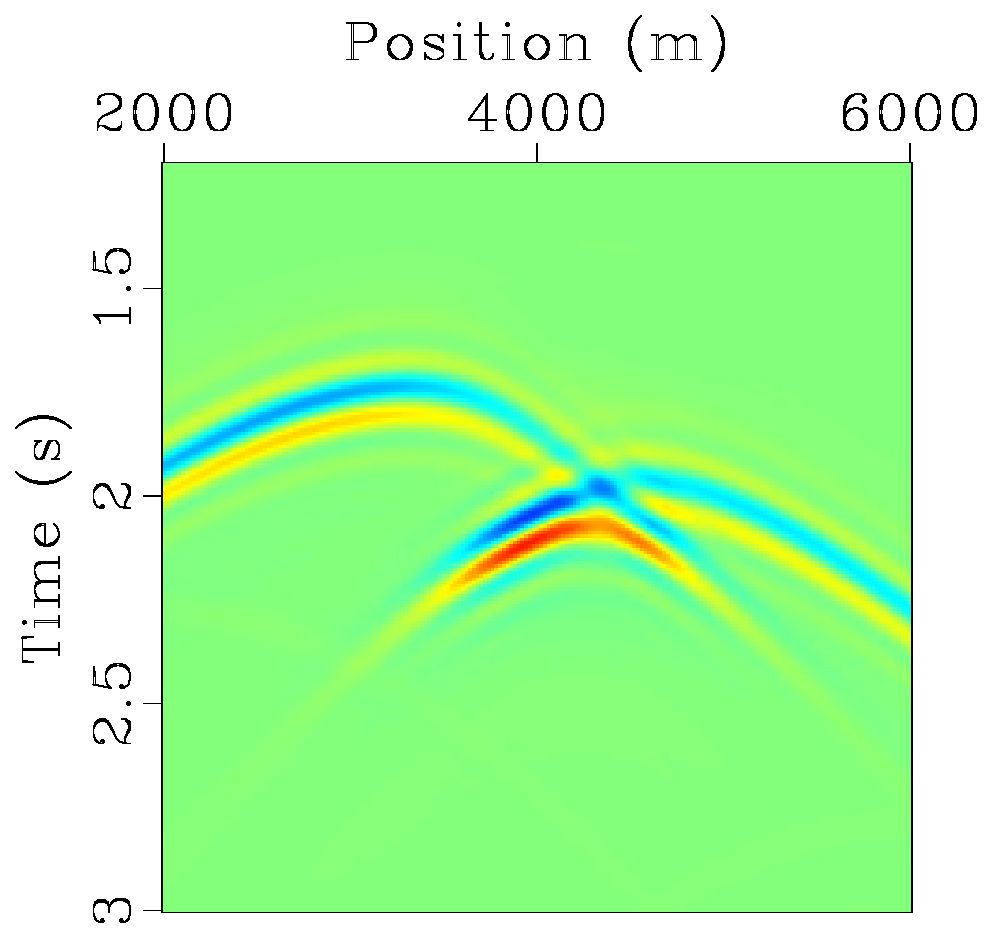
\includegraphics[width=0.45\textwidth]{dfwdvzlh0.pdf}}
  \subfloat[\label{fig:dinvhslh0}]{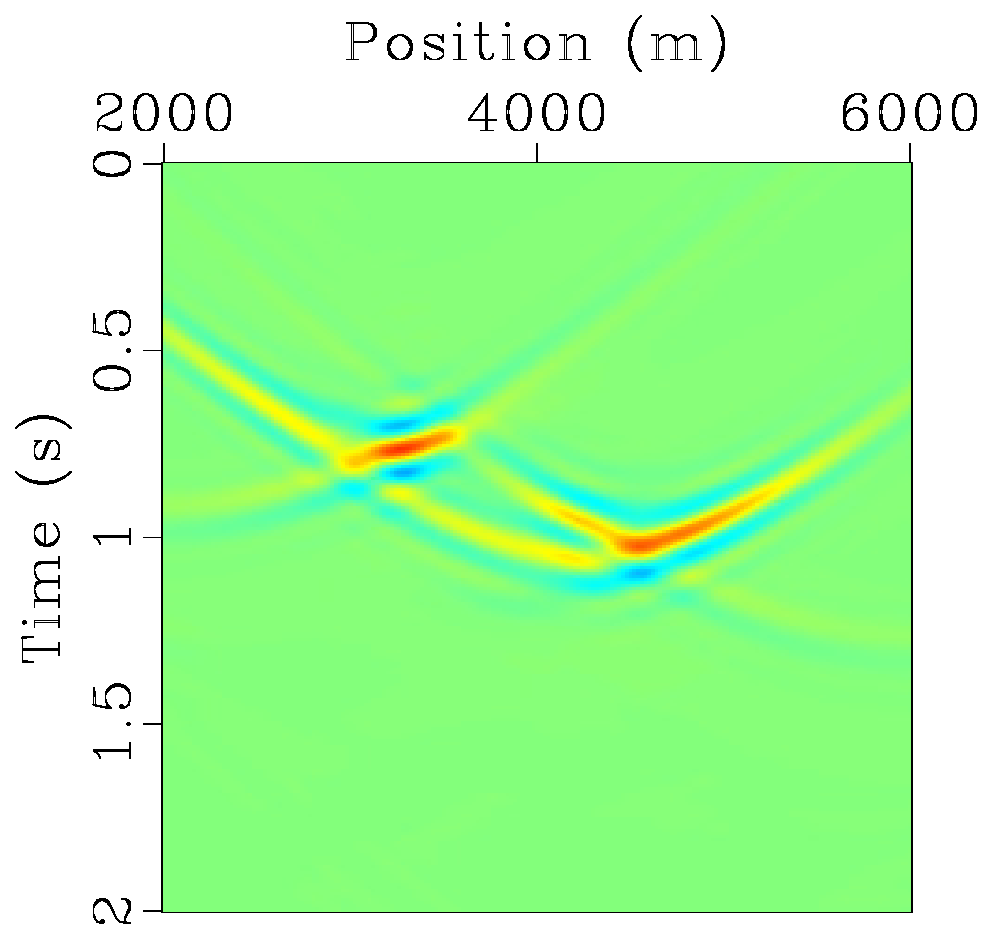
\includegraphics[width=0.45\textwidth]{dinvhslh0.pdf}}
  \caption{(a) Normal velocity data corresponding to pressure data in
    Figure \ref{fig:dfwdplh0}. (b) Source function resulting from time-reversal inversion
    of pressure data in Figure \ref{fig:dfwdplh0}. Propagation in homogeneous
    bulk modulus model (different from the model used to generate the
    data!). Plotted with same color scale as Figure \ref{fig:dsrcphh0}.}
\end{figure}

\begin{figure}
  \centering
  \subfloat[\label{fig:drerecplh0}]{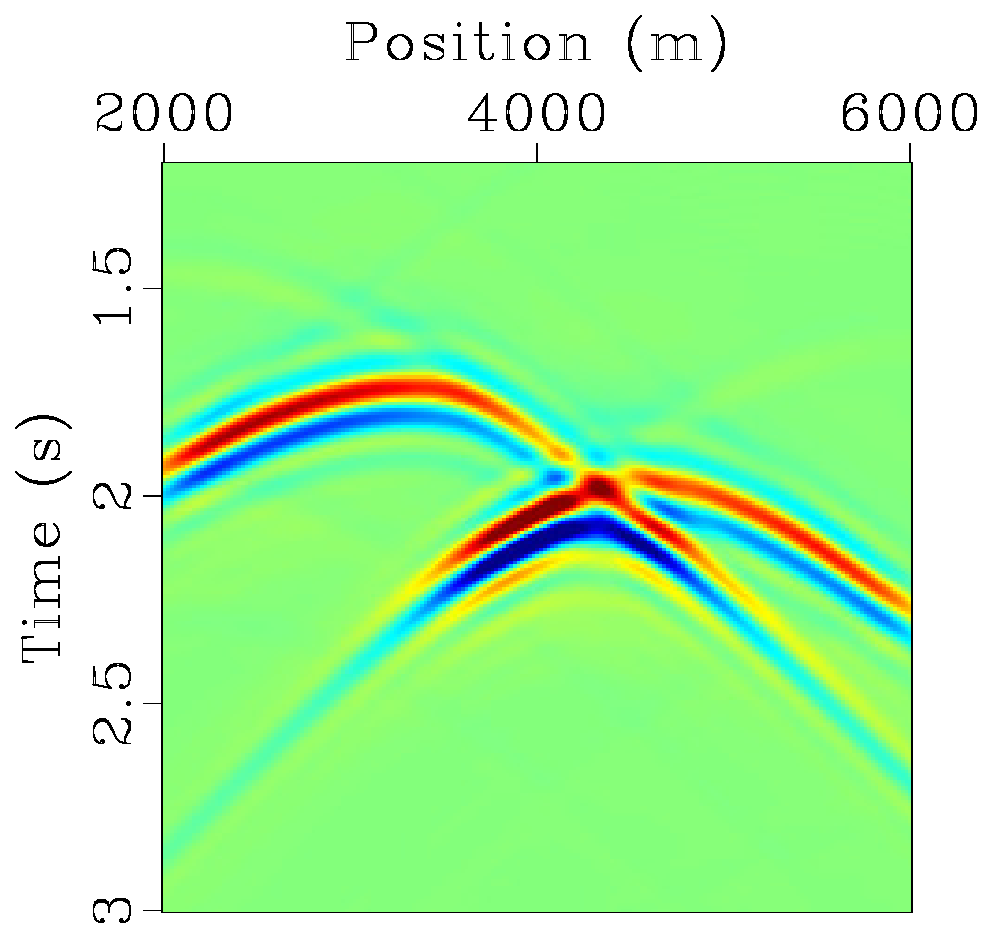
\includegraphics[width=0.45\textwidth]{drerecplh0.pdf}}
  \subfloat[\label{fig:ddiffrecplh0}]{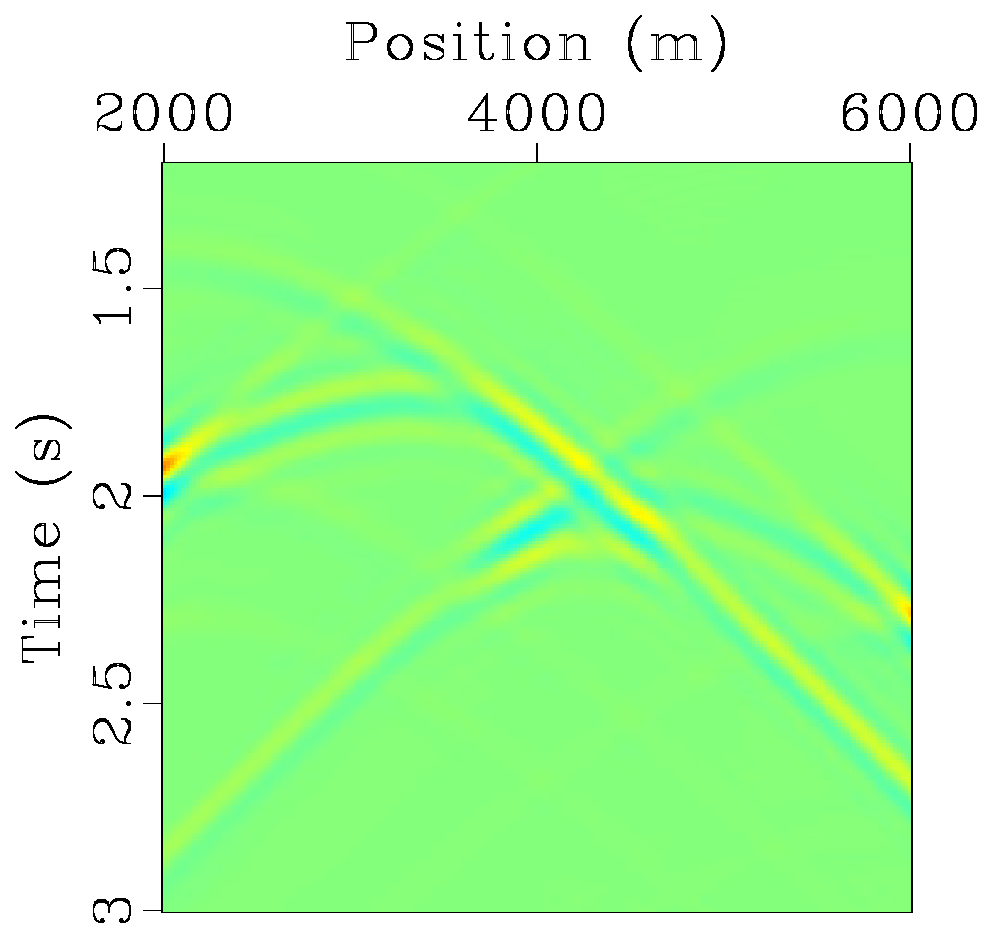
\includegraphics[width=0.45\textwidth]{ddiffrecplh0.pdf}}
  \caption{(a) Resimulated data: pressure gather generated from
    inverted source (Figure \ref{fig:dinvhslh0}), using same
    homogeneous bulk modulus as used in inversion. (b) Difference
    between data depicted in Figure \ref{fig:drerecplh0} and in Figure \ref{fig:dfwdplh0}.
    Both (a) and (b) plotted with same color scale as Figure \ref{fig:dfwdplh0}.}
\end{figure}
  
\subsection{Example: Diving Wave}

The second example is based on the diving wave model (Figure
\ref{fig:ooplrays0}). In this example, unlike the previous one, the source
and receiver surfaces do not bound the propagating region, even in the
vertical direction. Thus this exercise differs even more than the
first from time reversal in photoacoustic tomography. Inspection of
the blue part of the ray field in Figure \ref{fig:ooplrays0} reveals that
the rays are incoming at the source surface, and outgoing at the receiver surface, if the
outward normal is chosen as $-{\bf e}_z$. The mute shown in Figure
\ref{fig:ndwmute0} eliminates the rest of the ray field. What remains
satisfies the condition that every ray passing the receiver surface
originates in the source surface.

In this example, the inversion is performed with the same model as
used to generate the data. Note that sufficiently small changes in the model would
result in similar ray configurations, so time reversal inversion could
proceed as is shown here. However sufficiently large changes in the
bulk modulus model could result in fundamental changes in the ray
field: for instance, change to a homogenous model would completely
eliminate the diving rays and the corresponding data component, thus
making an inversion of the type presented here impossible. 

The inversion proceeds otherwise as before. The source $h_r=-2 P_rv_z$
on $\Sigma_r$ is built from the normal component of velocity, shown in
Figure \ref{fig:ndwdatavz0}. Reverse time propagation to create the
fields $(\tilde{p},\tilde{\bv})$, extraction of
the normal component of velocity (note the sign difference with the
previous example!) and scaling by the factor 2 produces the inverted
source shown in Figure \ref{fig:ndwdataresrcplbulksm0}. Forward
propagation yields the pressure gather shown in Figure
\ref{fig:ndwdataresimplbulksm0}, which closely matches the original
diving wave pressure data (Figure \ref{fig:ndwdata0}). The difference
is displayed on the same color scale in Figure
                    \ref{fig:ndwdatarediffplbulksm0}.

\begin{figure}
  \centering
  \subfloat[\label{fig:ndwdatavz0}]{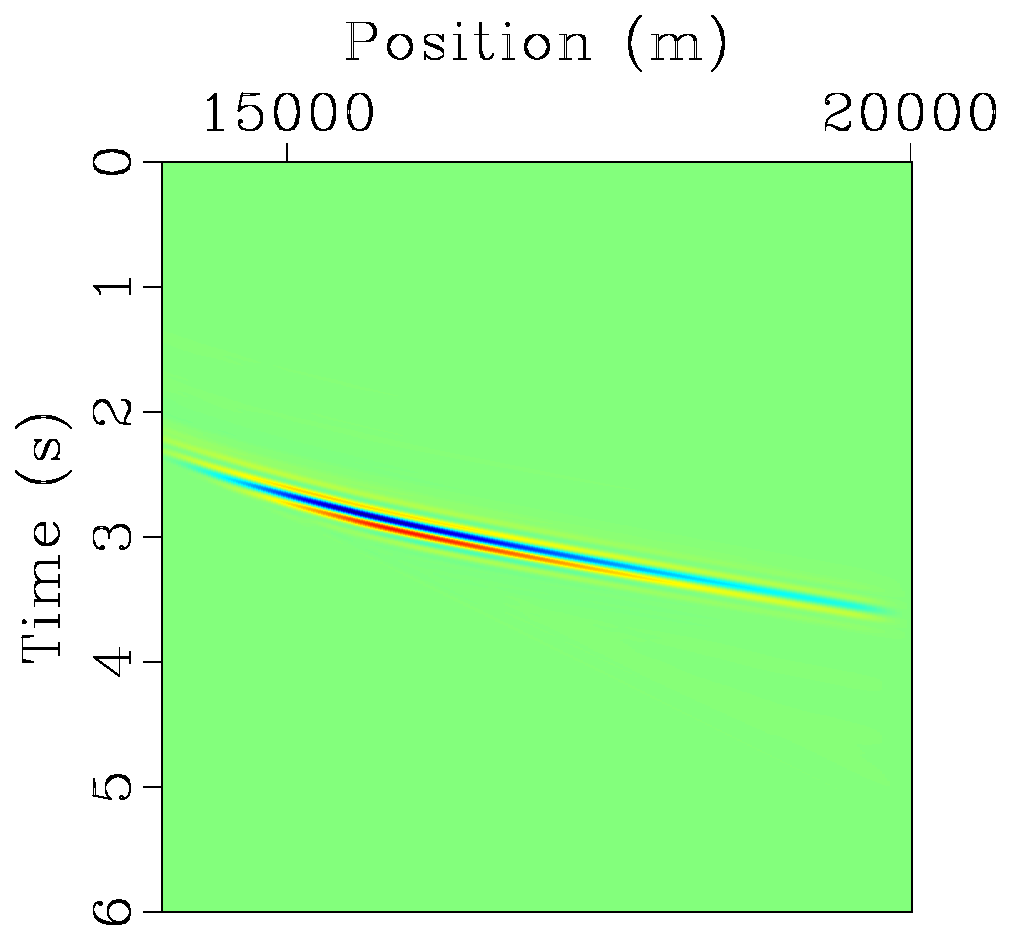
\includegraphics[width=0.45\textwidth]{ndwdatavz0.pdf}}
  \subfloat[\label{fig:ndwdataresrcplbulksm0}]{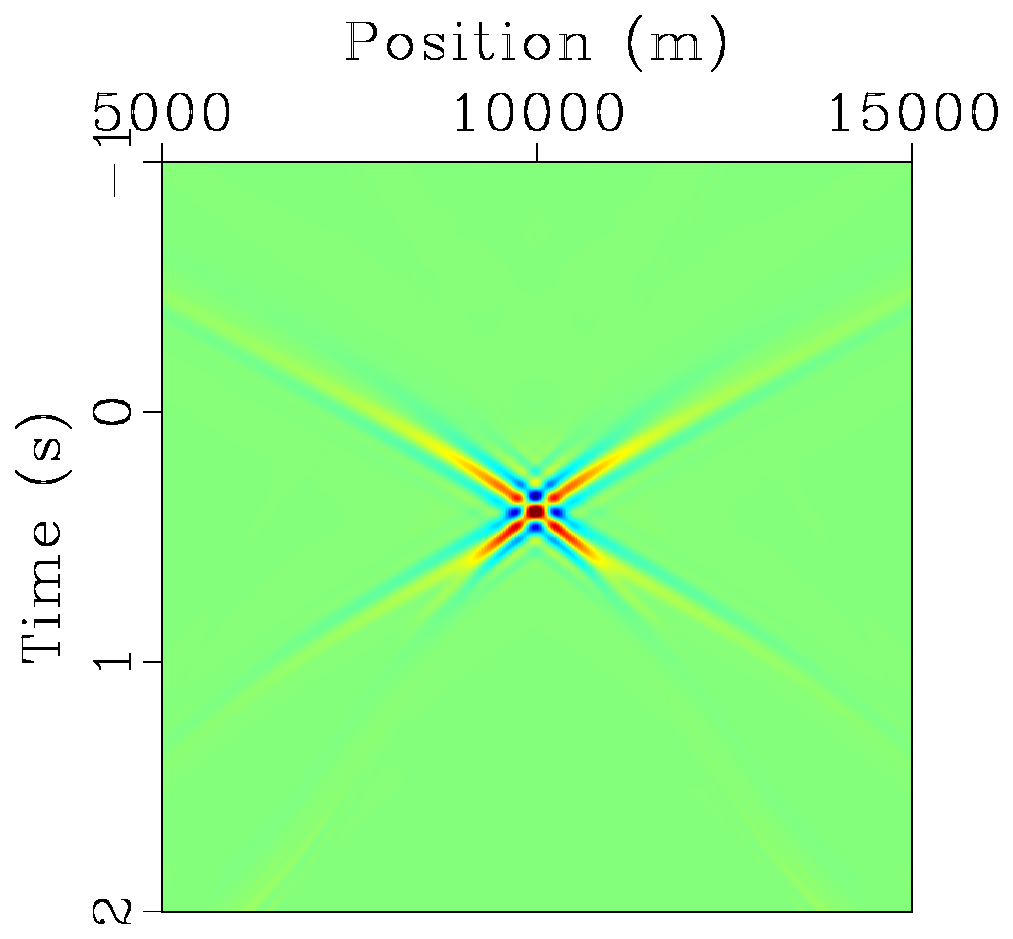
\includegraphics[width=0.45\textwidth]{ndwdataresrcplbulksm0.pdf}}
  \caption{(a) Normal velocity data corresponding to pressure data in
    Figure \ref{fig:ndwdata0}. (b) Source function resulting from time-reversal inversion
    of pressure data in Figure \ref{fig:ndwdata0}. Propagation in
    same model (Figure \ref{fig:ooplrays0}) as used to generate the data.}
\end{figure}

\begin{figure}
  \centering
  \subfloat[\label{fig:ndwdataresimplbulksm0}]{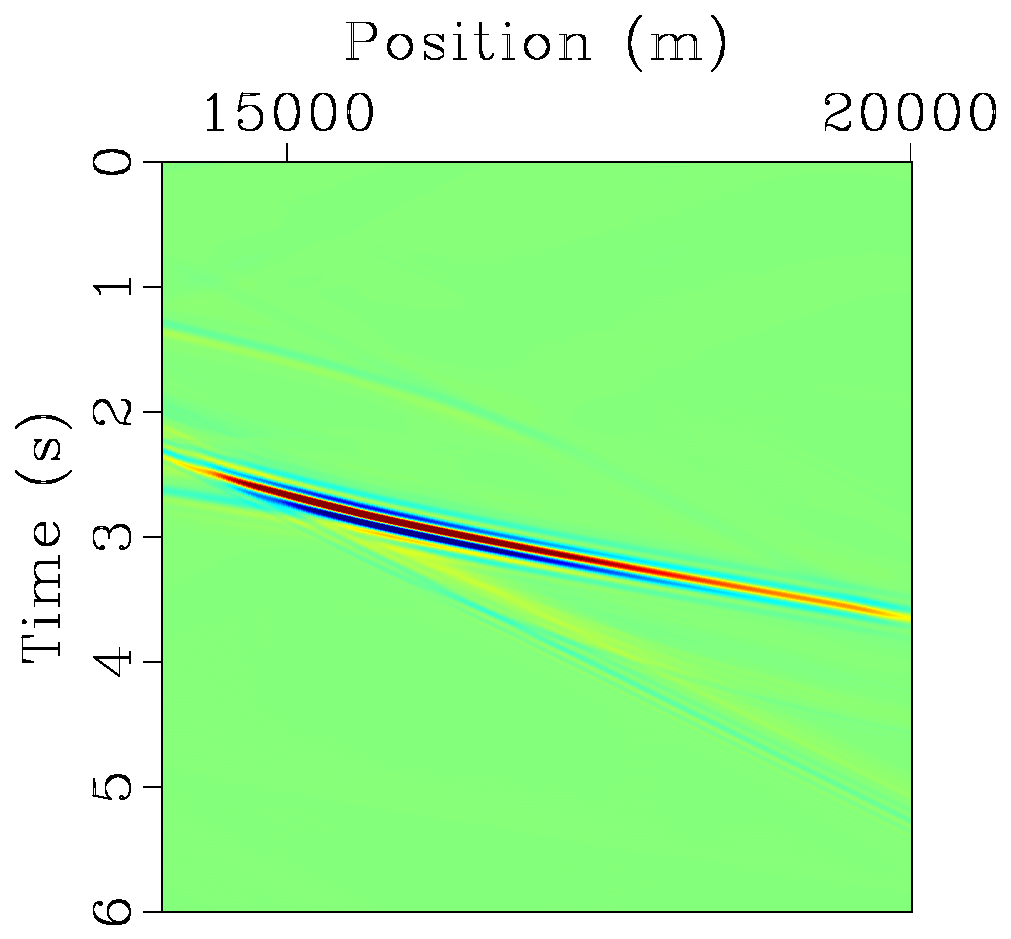
\includegraphics[width=0.45\textwidth]{ndwdataresimplbulksm0.pdf}}
  \subfloat[\label{fig:ndwdatarediffplbulksm0}]{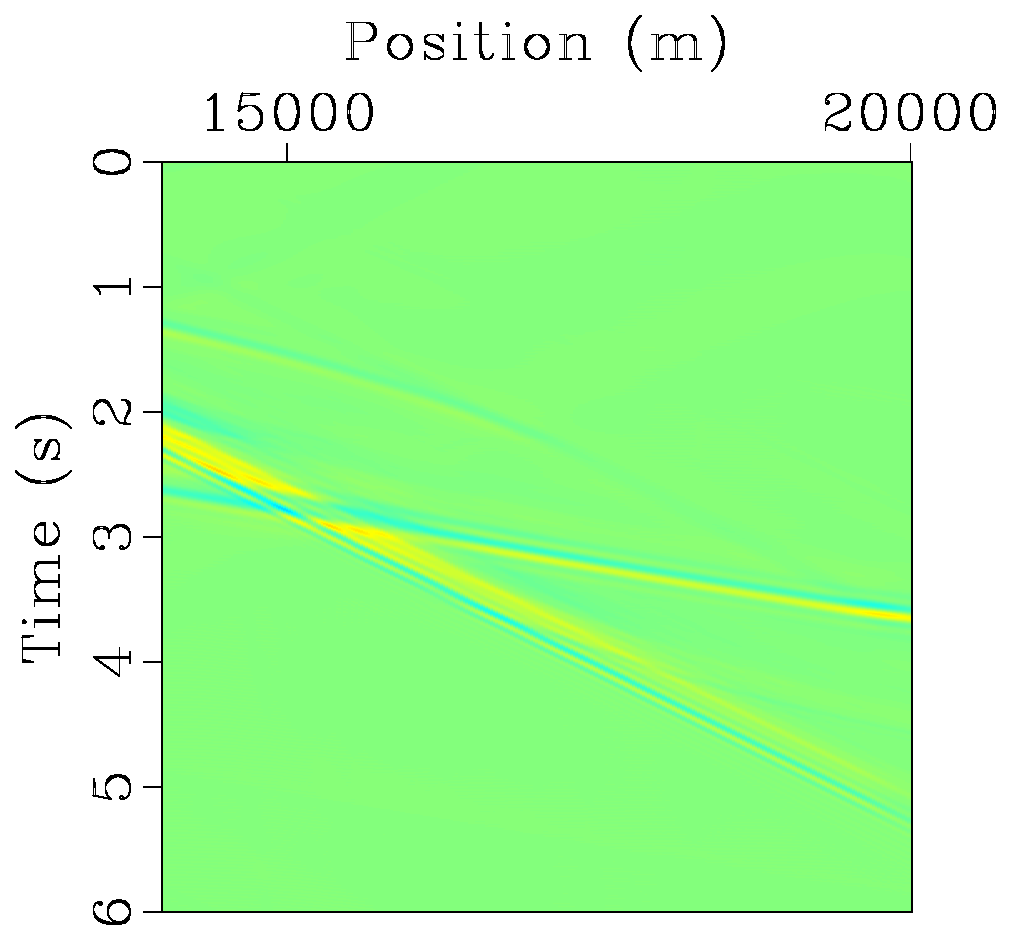
\includegraphics[width=0.45\textwidth]{ndwdatarediffplbulksm0.pdf}}
  \caption{(a) Resimulated data: pressure gather generated from
    inverted source (Figure \ref{fig:ndwdataresrcplbulksm0}), using same
    bulk modulus (Figure \ref{fig:ooplrays0}) as used in data
    generation and inversion. (b) Difference
    between data depicted in Figure \ref{fig:ndwdataresimplbulksm0} and in Figure \ref{fig:ndwdata0}.
    Both (a) and (b) plotted with same color scale as Figure
    \ref{fig:ndwdata0}. Note that low-amplitude ``ghosts'' of other
    arrival branches appear in the difference plot.}
\end{figure}

\section{Pressure-to-Source}

The result of the last section has a couple of apparent
defects. First, the approximate inversion of pressure data requires
knowledge of velocity data, which is not prescribed in the problem
statement \ref{eqn:esisp}. Second, the significance of the
reverse-time field $(\hat{p},\hat{\bv})$ is obscure. In this section
these two issues are addressed.

\subsection{Pressure-to-source operator}
The first step is to formalize the relation between pressure and
source (or equally well, pressure and normal velocity) on as surface
$\Sigma$ as the application of an operator.

Observe that in principle it's not necessary to
supply the normal velocity at the source (or receiver) surface, since
it's determined locally by the pressure on the surface, or causal (or
anti-causal) fields. This follows from the observation that the system
\ref{eqn:aweloc} has a unique solution, a by-product of the
conservation of energy (see for example \cite{Lax:PDENotes}, section
4.3). That is, in the language of that discussion, knowledge of $p$ on
$\Sigma$ for $0\le t \le \tau$ determines $(\tilde{p},\tilde{\bv})$ in
the entire domain $\Omega^+$, $0\le t \le \tau$. Therefore knowledge
of $p$ on $\Sigma$ for $0\le t \le \tau$ determines
$\bv \cdot {\bf n}$, up to a negligible error. As in the last section,
it follows that knowledge of $p$ on $\Sigma$, any $t$, determines a
source $h$ on $\Sigma$ for which the pressure field $\tilde{p}$
(solution of the system \ref{eqn:awesrcmod}) differs negligibly from
$p$.

This relation defines a causal {\em pressure-to-source operator}
$\Lambda: p \mapsto h$, yielding the source on a surface $\Sigma$ that
reproduces the (causal) pressure field from its trace on $\Sigma$, at
least locally on the inward side as defined by the selection of normal
field on $\Sigma$, under the ray conditions defined earlier. Since
$h \approx 2 \bv \cdot {\bf n}$ (limiting value of $\bv$ from the
inward direction), $\Lambda$ is effectively the
pressure-to-normal-velocity operator.

With this convention, two of the three steps in
the approximate inversion procedure are operator applications. The
operators involved are the causal pressure-to-source operator for the
source surface $\Sigma_s$, denoted $\Lambda_s$, and an analogous
anti-causal operator for the receiver surface $\Sigma_r$. 
The characterization of the the source field $h_r$ in equation
\ref{eqn:awerecglob} shows that this anti-causal pressure-to-source
operator differs from its causal analogue only by sign. Denote the
causal operator by $\Lambda_r$.

\subsection{Time Reversal as Adjoint State}
The middle step is solution of the reverse-time system
\ref{eqn:awerecglob} for the field $(\hat{p},\hat{\bv})$, with input
pressure source
$h_r$ on $\Sigma_r$ and output $P_s\hat{p}$ on $\Sigma_s$. To
understand the significance of this mapping, it is just as easy, and
will be useful later, to include a velocity source $f_r$, that is,
modify the second equation in \ref{eqn:awerecglob} by adding $f_r {\bf
  n}_r \delta_{\Sigma_r}$, so that it becomes a reverse-time version
of the basic system \ref{eqn:awepm}. Recall the definition of energy
in the acoustic field $(p,\bv)$:
\begin{equation}
  \label{eqn:energydef}
   E[p,\bv](t) = \frac{1}{2} \int \,dx\,dy\,dz\, \left(\frac{p(\bx,t)^2}{\kappa(\bx)} + \rho(\bx)\bv(\bx,t)
   \cdot \bv(\bx,t)\right)
\end{equation}
This is a quadratic form. Polarization makes a bilinear form, into
which one can plug a pair of fields. Use the solutions $(p,\bv)$ of
the forward-time system \ref{eqn:awepm} for one of the pair, and
the solution $(\hat{p},\hat{\bv})$ of system \ref{eqn:awerecglob}
(augmented with the velocity surface source) for the other. Since $(p,\bv)$ vanishes
for large negative time, $(\hat{p},\hat{\bv})$ for large positive
time, 
\[
0 = 
\left(\int\, dx\,dy\,dz\, \frac{p \hat{p}}{\kappa} +  
\rho \bv \cdot \hat{\bv} \right)|_{t \rightarrow \infty}
-
\left(\int\, dx\,dy\,dz\, \frac{p \hat{p}}{\kappa} +  \rho \bv \cdot \hat{\bv} \right)|_{t \rightarrow -\infty}
\]
\[
= 
\int_{-\infty}^{\infty} \,dt\, \frac{d}{dt}\left(\int\, dx\,dy\,dz\, \frac{p \hat{p}}{\kappa} +  \rho \bv \cdot \hat{\bv} \right)
\]
Carry out the differentiation under the integral sign, replace time derivatives by space derivatives and
source terms using the equations of motion in the systems
\ref{eqn:awepm} and \ref{eqn:awerecglob}, and integrate by parts to
move all of the space derivatives onto $p$ and $\bv$.  Most of the
remaining expressions cancel, leaving
\[
  = \int_{-\infty}^{\infty}\,dt \, \left[
    \int\,d\sigma_s(\bx)\,(h_sP_s\hat{p}+f_sP_s(\hat{\bv}\cdot{\bf
      n}_s)) +
    \int\,d\sigma_r(\bx)\,(h_rP_rp+f_rP_r(\bv\cdot{\bf n}_r)) \right]
\]
Here $\sigma_s$ and $\sigma_r$ are the area elements on $\Sigma_s$ and
$\Sigma_r$. These integrals are inner products of time traces on $\Sigma_s$ and $\Sigma_r$. Denote these inner products by $\langle \cdot,\cdot
\rangle_s$ and $\langle \cdot,\cdot
\rangle_r$ respectively. Then the above is written in terms of the
vector modeling operator ${\cal S}$ (definition \ref{eqn:fwd}) as 
\[
  = \langle (h_s,f_s)^T, (P_s\hat{p},P_s(\hat{\bv}\cdot{\bf
    n}_s))^T \rangle_s+ \langle (h_r,f_r)^T, {\cal S}(h_s,f_s)^T \rangle_r,
\]
whence identify the adjoint of ${\cal S}$ as
\begin{equation}
  \label{eqn:vecadj}
  {\cal S}^T(h_r,f_r) = -(P_s\hat{p},P_s(\hat{\bv}\cdot{\bf
    n}_s))^T.
\end{equation}
Specializing to the pressure modeling operator $S$ (equation
\ref{eqn:sdef}),
\begin{equation}
  \label{eqn:padj}
  S^T = (\Pi_0 {\cal S} \Pi_0^T)^T = \Pi_0 {\cal S}^T \Pi_0^T
\end{equation}
so to calculate the adjoint of $S$ applied to $h_r$, solve system
\ref{eqn:awerecglob} (with $f_r=0$) and extract the pressure at $\Sigma_s$:
\[
  S^T(h_r) = -P_s \hat{p}.
\]

Combined with the definitions of the pressure-to-source operators
$\Lambda_s$ and $\Lambda_r$, these results enable a translation of the
approximate inverse construction in the last section into a chain of
operator applications: to invert a pressure gather $d$ on $\Sigma_r$
for a source $h_s$ on $\Sigma_s$ that approximately reproduces it ($d
\approx Sh_s$),
\begin{itemize}
\item[1. ] create a source $h_r = -2\Lambda_r d$ on $\Sigma_r$;
\item[2. ] apply the adjoint $S^T$ (solve the reverse time system
  \ref{eqn:awerecglob}) to $h_r$;
\item[3. ] apply $\Lambda_s$ to $-S^Td$.
\end{itemize}
Putting this all together, an approximate right inverse operator
$S^{\dagger}$ to $S$ may be expressed as
\begin{equation}
  \label{eqn:baseinv}
  S^{\dagger} = \Lambda_s S^T \Lambda_r,
\end{equation}
that is,
\begin{equation}
  \label{eqn:rightinv}
  SS^{\dagger} \approx I.
\end{equation}

\subsection{Positivity of $\Lambda$}

Equation \ref{eqn:baseinv} is remarkable, in that the form of
$S^{\dagger}$ is that of an adjoint with respect to weighted norms,
defined by the operators $\Lambda_s^{-1}$ in the domain of $S$ and
$\Lambda_r$ in the range. This only makes sense if the
pressure-to-source operators are positive definite and symmetric, the
necessary conditions to define weighted norms. 

In fact the pressure-to-source operator is positive semi-definite, and that
fact has fundamental physical significance. Suppose that $(p,\bv)$
solves the basic system \ref{eqn:awepm} with $f_s=0$. From the
definition of energy \ref{eqn:energydef} and causality of the fields,
\[
 E[p,\bv](t_1) = \frac{1}{2} \int_{-\infty}^{t_1} \,dt \int \,dx\,dy\,dz\,
 \frac{d}{dt}\left(\frac{p(\bx,t)^2}{\kappa(\bx)} +
   \rho(\bx)\bv(\bx,t) \cdot \bv(\bx,t)\right)
\]
\[
  = \int_{-\infty}^{t_1} \,dt \int \,dx\,dy\,dz\,
 \left(\frac{p (\bx,t)\frac{\partial p}{\partial t}(\bx,t)^2}{\kappa(\bx)} +
   \rho(\bx)\bv(\bx,t) \cdot \partial{\bv}{\partial t}(\bx,t)\right)
\]
Using \ref{eqn:awepm}, replace the time derivatives with spatial derivatives and the delta
function on ths source surface, integrate by parts to shift the space
derivatives to $p$. Everything cancels except for
\[
  =  \int_{-\infty}^{t_1} \,dt \int \,dx\,dy\,dz\, p(\bx,t) h_s(\bx,t)
  \delta_{\Sigma_s}(\bx) = \int_{-\infty}^{t_1} \,dt \int_{\Sigma_s} \,d\sigma_s \, p h_s.
\]
Take the limit as $t_1 \rightarrow \infty$ to get
\[
\lim_{t_1 \rightarrow \infty} E[p,\bv](t_1) = \langle h_s, P_s p \rangle_s = \langle P_s p, \Lambda_s P_s p \rangle_s. 
\]
That is, the value of the quadratic form defined by
$\Lambda_s$, evaluated at the pressure trace on $\Sigma_s$,
gives the total energy transferred from the source to the
acoustic field over time. Since $E$ is itself a positive definite
quadratic form in the acoustic field, it follows that $
\Lambda_s$ is positive semi-definite. 

\subsection{Approximate symmetry of $\Lambda$}
Except in special cases, $\Lambda_{s,r}$ is not
symmetric. However, it is {\em approximately symmetric} in the
high-frequency sense. This fact follows from a high-frequency
asymptotic analysis, a sketch of which follows for the special case of
a planar source surface
$\Lambda_s=\{z=z_s\}$, as in the two examples. Since the same reasoning
applies to $\Lambda_r$, I will omit the subscript for the remainder of
this subsection.

The pressure trace
$p(x,y,t)$ can be expressed by Fourier synthesis as
\begin{equation}
  \label{eqn:four}
p(x,y,t) = \frac{1}{(2\pi)^3}\int \,d \omega \,d\xi \, d\eta \,\omega^2
\,d\eta\,\hat{p}(\omega,\xi,\eta) e^{i\omega(t-x\xi - y\eta)}
\end{equation}
in which the spatial frequencies have been expresed as slownesses
$\xi,\eta$ scaled by temporal frequency $\omega$.
Choose $a_0(x,y,t)$ so that $a_0(x,y,t) = 1$ if $p(x,y,t) \ne 0$. Then
$p(x,y,t) = a_0(x,y,t)p(x,y.t)$
\begin{equation}
  \label{eqn:fourloc}
=\frac{1}{(2\pi)^3}\int \,d\omega \, d\xi \, d\eta \, \omega^2
\,d\eta\,\hat{p}(\omega,\xi,\eta) [a_0(x,y,t) e^{i\omega(t-x\xi -
  y\eta)}]
\end{equation}
This identity expresses $p(x,y,t)$ as a sythesis of
oscillatory wave packets of the form
\begin{equation}
  \label{eqn:pwp}
 a_0(x,y,t) e^{i\omega(t-x\xi-y\eta)}
\end{equation}
in which the spatial frequencies have been expressed as slownesses
$\xi,\eta$ scaled by temporal frequency $\omega$. The function $a_0$
is a frequency-independent envelope, equal to 1 where $h$ is
non-zero.

The wave packet $a_0(x,y,t) e^{i\omega(t-x\xi-y\eta)}$ can be
viewed as the boundary value on $\Sigma$ of a
high-frequency asymptotic solution of the form \ref{eqn:go}, provided that the
slowness vector $(\xi, \eta)$ satisfies the propagating condition
$c^2(\bx)(\xi^2+\eta^2) < 1$ at all $\bx$ for
which $a_0(\bx,t)$ is non-zero for any $t$. [In general, this is a
strong condition, and might not even have any solutions. However it
always has solutions if $a_0(x,y,t)$ is nonzero only over a sufficiently
small region, which is the case is $p(x,y,t)$ is non-zero over a
sufficiently small region. An arbitrary $p(x,y,t)$ can always be
broken up into a sum, the summands of which are non-zero only over
small regions, so in fact the requirement mentioned above is not a
significant constraint: just carry out the following construction for
summands, and add up the results.] In that case, two
solutions $\psi$ of the eikonal equation $|\nabla \psi|=c$ exist, at least locally near
$\Sigma$, for which $\psi(x,y,0)=x\xi+y\eta$. Choose the solution
that increases in the direction of the outward unit normal ${\bf
  n}$, and solve the corresponding transport equation for an
amplitude $a$ satisfying $a(x,y,0,t) = a_0(x,y,t)$. Then the geometric optics solution $a e^{i\omega(t-\psi)}$ is
asymptotic to the pressure field of an incoming solution. From the
evolution equation for $\bv$, integrated in time as in equation
\ref{eqn:newt},  an expression follows for the corresponding normal
velocity:
\[
  -{\bf n} \cdot \frac{1}{\rho}\int_{-\infty}^t ds \nabla (a
  e^{i\omega(s-\psi)})=\frac{1}{\rho}\int_{-\infty}^t ds {\bf n}
  \cdot(i\omega a\nabla \psi -\nabla a) e^{i\omega(s-\psi)})
\]
Now use the identity
\[
  e^{i\omega(s-\psi)} = \frac{1}{i\omega}\frac{d}{ds}e^{i\omega(s-\psi)}
\]
and integrate by parts in $s$ to obtain the expression for
the normal velocity field 
\[
  = \frac{a}{\rho} ({\bf n} \cdot \nabla \psi)  e^{i\omega(t-\psi)} + O(1/\omega).
\]
The terms not written explicitly begin with one of order -1 in
$\omega$. The remainder appears to be also of order -1, but
application of the integration-by-parts trick described above yields
another term of order -2 plus another remainder of apparent order
-2. Continuing this process develops the $O(1/\omega)$ remainder in an
asymptotic series of homogeneous terms in $1/\omega$ of arbitrary
length.

An expression for the normal velocity on
$\Sigma$ follows by restriction. Note that ${\bf n} \cdot \nabla \psi =( c^{-2}(x,y,z)-
(\xi^2+\eta^2))^{1/2}$ because of the choice of sign and the eikonal
equation, and the root is real because of the propagating assumption.

The upshot of this calculation is that to leading order in frequency,
the normal velocity corresponding to a pressure wave packet differs by a position- and slowness-dependent
factor. Accounting for the factor of 2 difference between the source
amplitude and velocity trace, this calculation may be summarized:
\begin{equation}
  \label{eqn:lamwp}
  \Lambda (a_0e^{i\omega(t-x\xi-y\eta)}) = \lambda
  (a_0e^{i\omega(t-x\xi-y\eta)}),
\end{equation}
where $\lambda(x,y,t,\xi,\eta,\omega)$ is
defined by the asymptotic series in $\omega$ developed above. Its dominant term,
$O(1)$ (order 0) in $\omega$, is
\[
  \lambda^0(x,y,t,\xi,\eta,\omega) = 2\frac{( c^{-2}(x,y,z)-
    \xi^2+\eta^2)^{1/2}}{\rho} + O(1/\omega)
\]
\begin{equation}
  \label{eqn:lamsymb}
= 2(\kappa
\rho)^{-1/2}\left(1-\frac{\kappa(k_x^2+k_y^2)}{\rho \omega^2}\right)^{1/2} + O(1/\omega).
\end{equation}
In the final expression, the slownesses $\xi,\eta$ have been replaced
by the Fourier variables $k_x=x\xi, k_y=y\eta$. Note that as a
function of $k_x,k_y,\omega$, $\lambda^0$ is homogeneous of order
0. It is easy to see that the $N$th term of the asymptotic series
defining $\lambda$ is of homogeneous order $-N$.

%%%%%%%%%%%
% discussion of psidos
%
Operators that affect oscillatory wave packets by multiplication with
functions having the properties of $\lambda$ have come to
be called ``pseudodifferential'' \cite[]{Nir:72,Tay:81,SaiR:91}. The multiplier ($\lambda$ in this
case) is called the {\em symbol} of the operator, and the dominant
term in an asymptotic development of the multiplier
(for instance $\lambda^0$) is called the {\em principal symbol}.
Amongst other special properties of these operators, their adjoints
are operators of the same type. In particular, the principal symbol of the adjoint is
the Hermitian (matrix) adjoint of the principal symbol. For scalar
operators like $\Lambda$ (mapping scalar-valued functions to
scalar-valued functions), the symbols are scalar ($1 \times 1$), and
the Hermitian adjoint is simply the complex conjugate (\cite{Tay:81},
section II.4). Therefore scalar operators with real principal symbol,
like $\Lambda$, have the same principal symbols as their adjoints. So
$\Lambda$ differs from $\Lambda^T$ by a pseudodifferential operator
whose symbol is an asymptotic sum of terms of negative order in
frequency. Therefore the difference is negligible in the limit of high
frequencies. This observation establishes the conclusion of this subsection: 
\begin{equation}
  \label{eqn:lamappsim}
  \Lambda^T \approx \Lambda,
\end{equation}

Before leaving this topic, recall that the computation outlined above
was predicated on the propagating assumption, namely that the slowness
parameters $\xi,\eta$ of the wave packet defined in \ref{eqn:pwp}
satisfy $c(x,y,z_s)^2(\xi^2 + \eta^2) < 1$ whereever the amplitude
$a_0(x,y,t)$ is non-zero. Therefore the conclusion \ref{eqn:lamappsim}
holds only for application to such wave packets. However, the restriction of
propagating waves (such as those that are output by the modeling
operator $S$ or its adjoint $S^T$) are well-approximated by sums over
propagating wave packets: this is part of the assumption that the rays
carrying high-frequency energy cross the source and receiver surfaces
at non-zero angles. To make the definition of $\Lambda$ complete, it
must be extended to non-propagating wave packets, for instance by
making its effect negligible via a dip filter. I will ignore this refinement, since the
application to non-propagating components appears to play little role
in approximate inversion and its applications as developed here.

\section{Computing $\Lambda$}

The missing ingredient in the preceding discussion is any indication
of how the action of the pressure-to-source operators $\Lambda$ is to be
computed. As will be seen in the next section, an (approximate)
inverse of this operator is also required in the formulation of
preconditioned Krylov iteration. 

Direct computation of the pressure-to-source operator $\Lambda_s$, for instance, by solving
\ref{eqn:awepm} and reading off $P_sv_{z}$, turns out to be
numerically ill-behaved. An alternate approach begins with the
observation that a pressure gather on $\Sigma_r$ produced by a
pressure source $h_s$ on $\Sigma_s$ can also be well-approximated by
the field from a velocity source. To see this, recall the first major
step in the time reversal construction, that a solution of the wave
equation near $\Sigma_s$ can be represented as the solution of a
boundary value problem with $p$ given on $\Sigma_s$ (system
\ref{eqn:aweloc}). The derivation combined the unique determination of
the field by its pressure boundary values on an enclosing domain with
the consequences of the standing assumptions about rays carrying high
frequency energy. Precisely the same logic could have been applied to
the normal velocity boundary values, as these also uniquely determine
the field in an enclosing domain. Proceeding further, a source
representation based on continuous extension of normal velocity, with
a jump in the pressure follows by logic precisely analogous to that
leading to the system \ref{eqn:awesrc}: instead, obtain a field
$(\tilde{p},\tilde{\bv})$ differing negligibly from the field of the
same name in the earlier discussion, solving 
\begin{eqnarray}
\label{eqn:awesrcvzmod}
  \frac{1}{\kappa}\frac{\partial\tilde{p}}{\partial t} & = & 
                                                      - \nabla \cdot \tilde{\bv}, \nonumber \\
  \rho\frac{\partial \tilde{\bv}}{\partial t} & = & f_s {\bf n}\delta_{\Sigma}- \nabla \tilde{p}, \nonumber \\
  \tilde{p} & = & 0 \mbox{ for }  t \ll 0, \nonumber \\
  \tilde{\bv} & = & {\bf 0} \mbox{ for }  t \ll  0.       
\end{eqnarray}
(that is, system \ref{eqn:awepm} with $h=0$) with $f_s = 2P_sp$.

This fact can usefully be rewritten using the vector modeling
operator ${\cal S}$ (definition \ref{eqn:fwd}), and the projection
operators $\Pi_i$ (definition \ref{eqn:pidef}), which insert scalar
sources into the pairs that occur in the acoustic system
\ref{eqn:awepm}: explicitly, $\Pi_0(h,f)^T = h, \Pi_1(h,f)^T = f,
\Pi_0^Th = (h,0), \Pi_1^Tf = (0,f)$. Then
\begin{eqnarray}
  P_r\tilde{p} &=& \Pi_0 {\cal S} \Pi_1^Tf_s, \nonumber \\
  P_r({\bf n}_r \cdot \tilde{\bv}) &=& \Pi_1 {\cal S} \Pi_1^Tf_s.
                                       \label{eqn:ptildef}
\end{eqnarray}
Since the field $(\tilde{p},\tilde{\bv})$ constructed here differs negligibly from that
constructed earlier with the same name, which in turn differs negligibly from $p$, it
follows that $P_r\tilde{p} \approx P_rp = Sh_s$. By definition of $S$
(\ref{eqn:sdef}), this is the same as $=\Pi_0{\cal
  S}\Pi_0^Th_s$. Since the velocity fields also differ negligibly,
obtain
\begin{eqnarray}
  P_r\tilde{p} & \approx & \Pi_0 {\cal S} \Pi_0^Th_s, \nonumber \\
  P_r({\bf n}_r \cdot \tilde{\bv}) & \approx & \Pi_1 {\cal S} \Pi_0^Th_s.
                                       \label{eqn:ptildeh}
\end{eqnarray}

From the definition of $\Lambda_s$, $h_s=\Lambda_sP_sp =
\frac{1}{2}\Lambda_sf_s$. Combining \ref{eqn:ptildef},
\ref{eqn:ptildeh}, and this last identity, obtain
\begin{equation}
  \label{eqn:snull}
  {\cal S}\left(-\frac{1}{2}\Lambda_{z_s}f_s,f_s\right)^T \approx 0.
\end{equation}

That is, the same data gather on $\Sigma_r$ can be obtained either
with a pressure source $h_s$ or with a velocity source $f_s$, and
there is a definite relation betwen the two. To illustrate this
relation, recall that for the first of the two examples introduced
above, the velocity source $f_s$ is twice the pressure trace shown in
Figure \ref{fig:dsrcphh0}, and the pressure source (Figure \ref{fig:dhshh0}) is twice the normal
velocity trace shown in Figure \ref{fig:dsrcvzhh0}.
Figure \ref{fig:daltplh0} shows $\Pi_0{\cal S}\Pi_1^Tf_s$, Figure
\ref{fig:dfwdplh0bis} shows $\Pi_0{\cal S}\Pi_0^Th_s$, and Figure
\ref{fig:ddifffwdaltplh0} shows the difference on the same color scale.

\begin{figure}
  \centering
  \subfloat[\label{fig:dsrcphh0}]{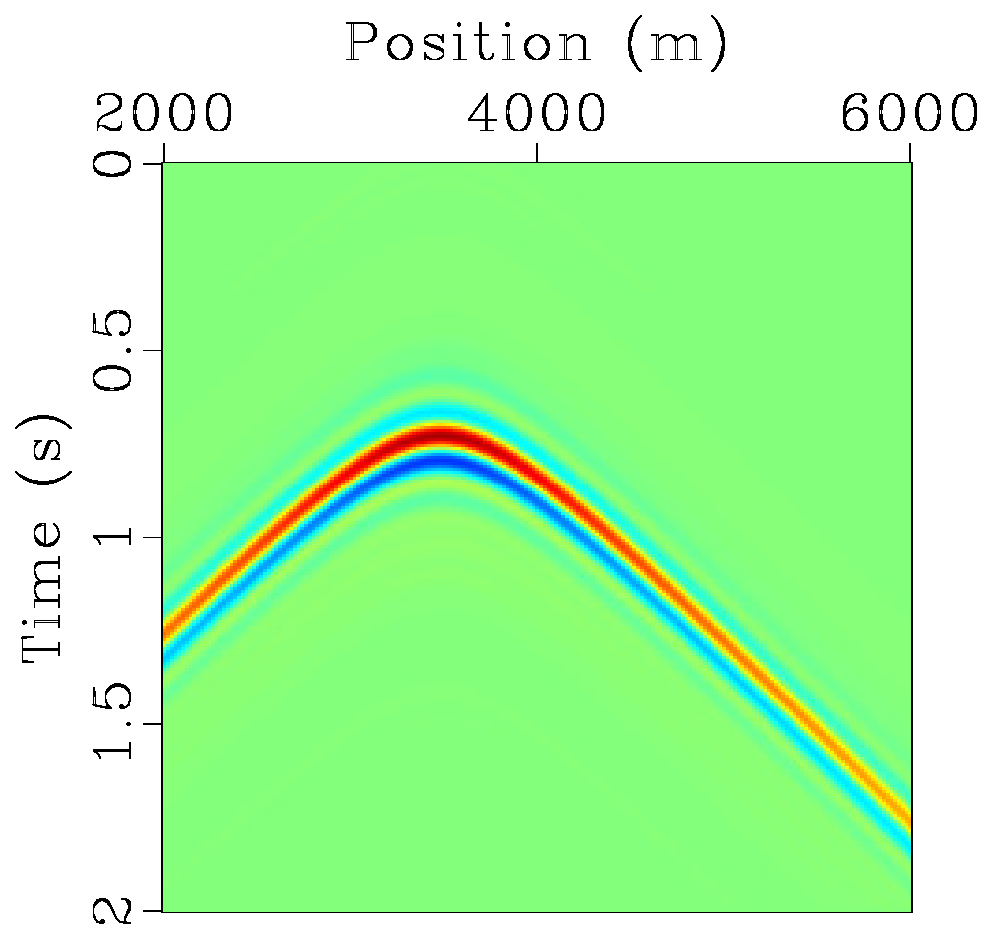
\includegraphics[width=0.45\textwidth]{dsrcphh0.pdf}}
  \subfloat[\label{fig:dsrcvzhh0}]{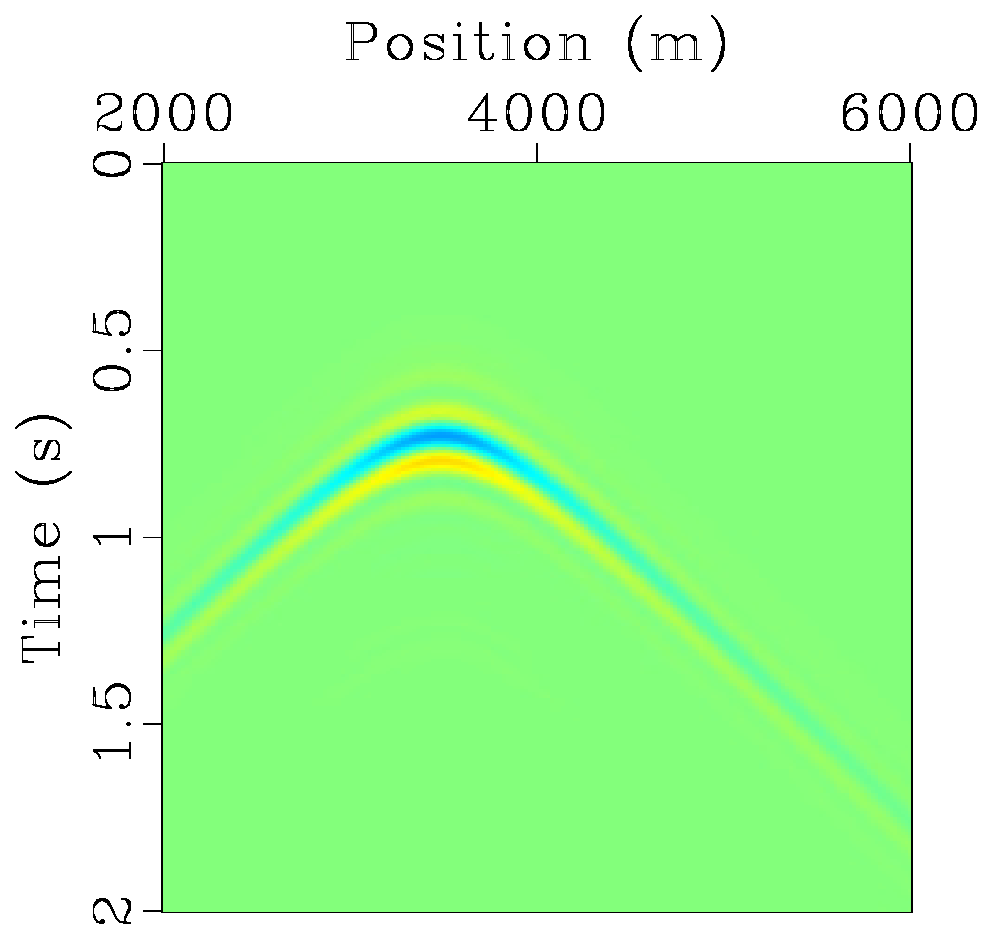
\includegraphics[width=0.45\textwidth]{dsrcvzhh0.pdf}}
  \caption{(a) Pressure gather for Lens example on source surface
    $\Sigma_s=\{z=1000\mbox{ m}\}$, generated by point source at
    $(3500,3500)$ m. (b) Normal velocity gather for Lens example on source surface
    $\Sigma_s=\{z=1000\mbox{ m}\}$, generated by point source at
    $(3500,3500)$ m.}
\end{figure}

\begin{figure}
  \centering
  \subfloat[\label{fig:dfwdplh0bis}]{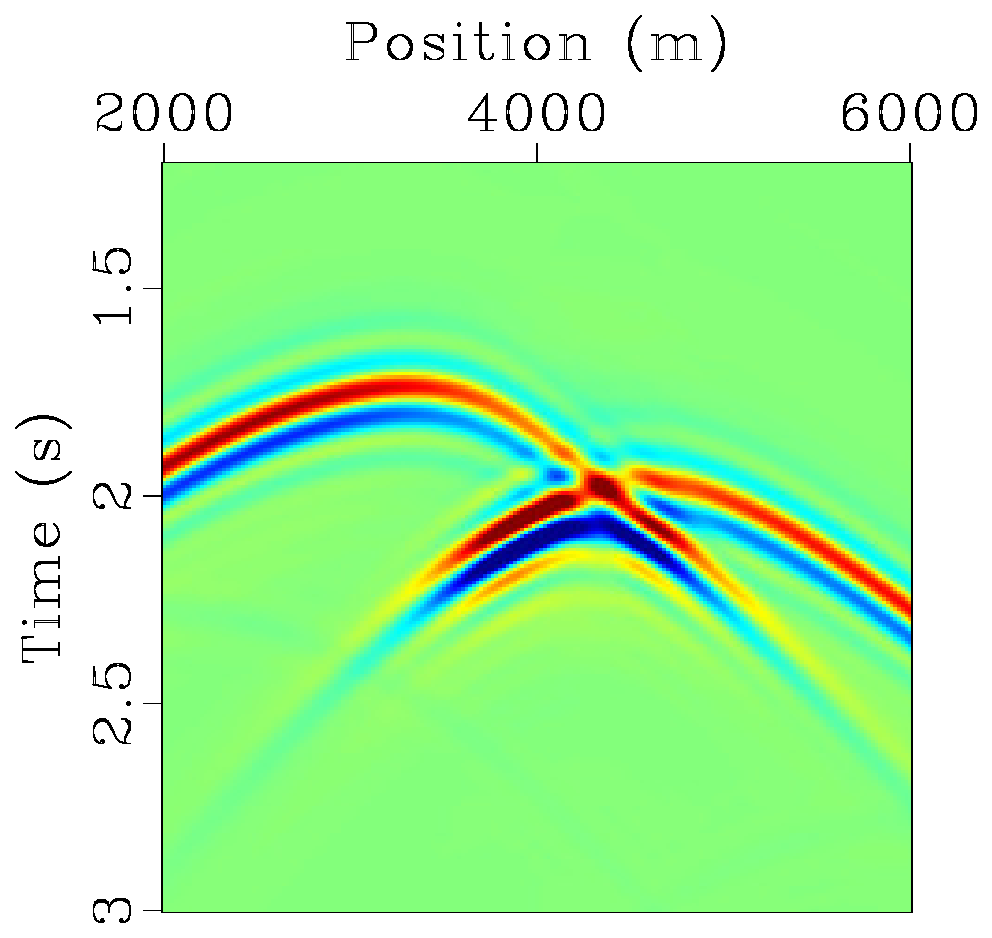
\includegraphics[width=0.32\textwidth]{dfwdplh0.pdf}}
  \subfloat[\label{fig:daltplh0}]{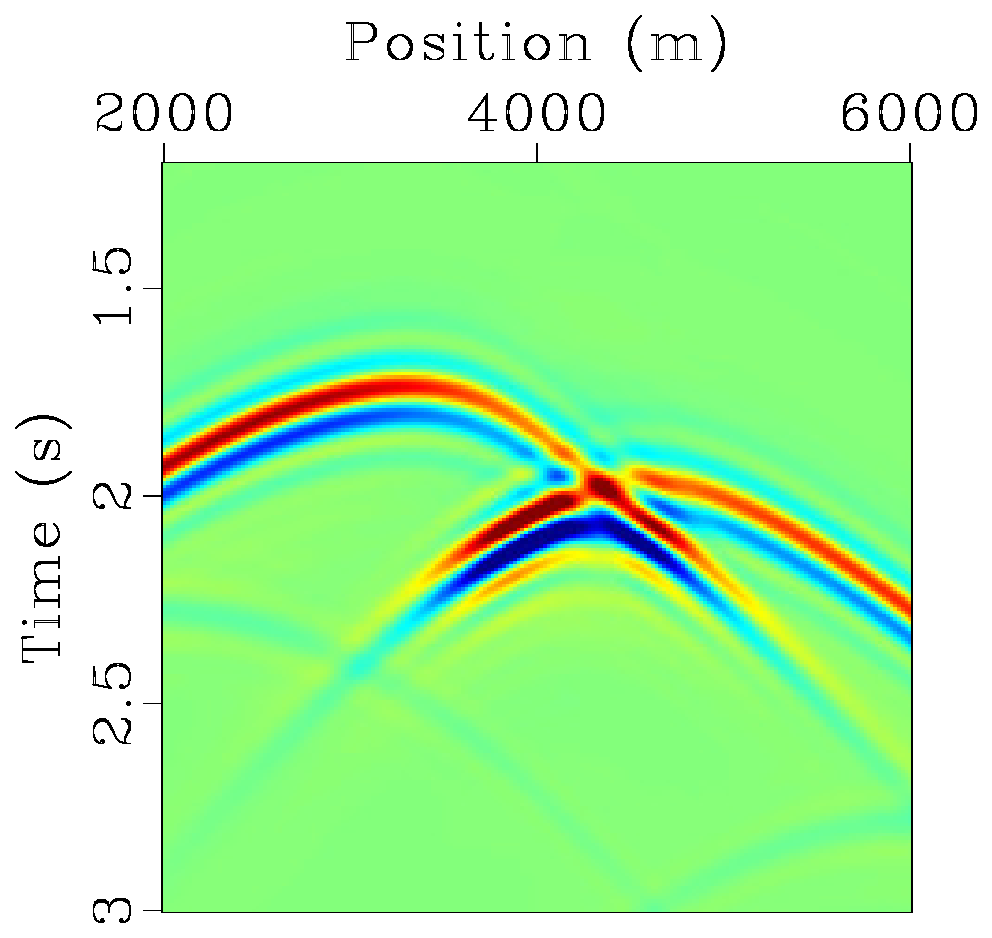
\includegraphics[width=0.32\textwidth]{daltplh0.pdf}} 
  \subfloat[\label{fig:ddifffwdaltplh0}]{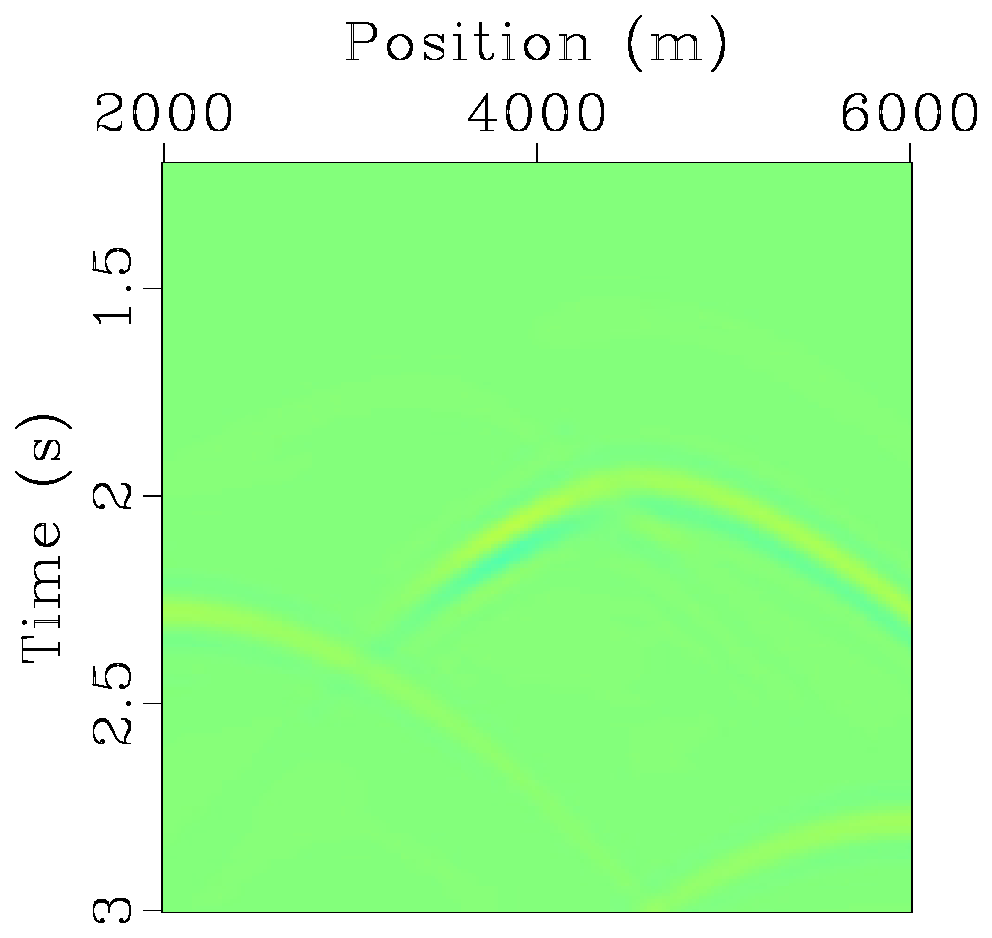
\includegraphics[width=0.32\textwidth]{ddifffwdaltplh0.pdf}}
  \caption{(a) Pressure gather on receiver surface
    $\Sigma_r=\{z=1000\mbox{ m}\}$ due to extended pressure source = 2
    $\times$ normal velocity gather shown in Figure
    \ref{fig:dsrcvzhh0}. This is the same gather as shown in Figure
    \ref{fig:dfwdplh0}, and the extended pressure source has been
    shown in Figure \ref{fig:dhshh0}.
    (b) Pressure gather on receiver surface
    $\Sigma_r=\{z=1000\mbox{ m}\}$ due to extended velocity source = 2
    $\times$ pressure gather shown in Figure
    \ref{fig:dsrcvzhh0}. (c) Difference (b)-(a), plotted on same color
    scale.}
\end{figure}

One other important consequence of this duality is an alternate view
of the time reversal construction of the approximate inverse. The
entire construction can be carried out with traces of the normal
velocity in place of trace of the pressure. The steps are precisely
analogous, and justified in exactly the same way. Therefore I will
simply summarize the result:
to invert a pressure gather $d$ on $\Sigma_r$
for a source $f_s$ on $\Sigma_s$ that approximately reproduces it ($d
\approx \Pi_0{\cal S}\Pi_1^Tf_s$):
\begin{itemize}
\item[1. ] create a source $f_r = - 2d$ on $\Sigma_r$;
\item[2. ] apply the adjoint $(\Pi_1{\cal S}\Pi_1^T)^T=\Pi_1{\cal
    S}^T\Pi_1^T$ (solve the reverse time system
  \begin{eqnarray}
  \label{eqn:awerecglobvz}
  \frac{1}{\kappa}\frac{\partial\hat{p}}{\partial t} & = & 
                                                      - \nabla \cdot \hat{\bv}, \nonumber \\
  \rho\frac{\partial \hat{\bv}}{\partial t} & = & f_r {\bf n}r
  \delta_{\Sigma_r} - \nabla \hat{p}, \nonumber \\
  \hat{p} & = & 0 \mbox{ for } t\gg 0, \nonumber \\
    \hat{\bv} & = & {\bf 0} \mbox{ for } t \gg 0.
  \end{eqnarray}
\item[3. ]
  then extract $h_s=2{\bf n_s}\cdot P_s\hat{\bv}. = 2\Pi_1{\cal
    S}^T\Pi_1^Tf_r=-4\Pi_1{\cal S}^T\Pi_1^Td$.
\end{itemize}
The upshot of this construction is the alternate computation for the
approximate inverse:
\begin{equation}
  \label{eqn:altinv}
  S^{\dagger}  \approx -4\Pi_1{\cal S}^T\Pi_1^T.
\end{equation}
The first row of
\ref{eqn:snull}, slightly rearranged, reads
\begin{equation}
  \label{eqn:lamidea}
  \Pi_0{\cal S}\Pi_1^T f_s \approx  \frac{1}{2} S\Lambda_sf_s.
\end{equation}
Apply the approximate inverse construction in the form
\ref{eqn:altinv} to solve \ref{eqn:lamidea} for $\Lambda_s$:
\begin{equation}
  \label{eqn:lamident}
  \Lambda_s \approx -8\Pi_1{\cal S}^T\Pi_1^T\Pi_0 {\cal S}\Pi_1^T.
\end{equation}
This identity is the major result of this section: it shows how
to compute that action of $\Lambda_s$ by propagating the input
pressure trace, identified as a source for the velocity evolution,
forward in time 
reading off the pressure trace on $\Sigma_r$, identifying it once more as
a point load (source for velocity), propagating it backwards in time, and finally reading off the velocity trace, scaled to be a
pressure evolution source on $\Sigma_s$. 

The importance of this result lies in the failure of the obvious
method for computing the action of $\Lambda_s$, namely to
employ the pressure trace as a source in the velocity equation ($f_s$,
in the notation used above) at $\Sigma_s$, and read off the velocity
field also at $\Sigma_s$. This difficulty is related to the existence of
tangentially propagating waves and the lack of continuity of the trace
operator. The method implicit in equation \ref{eqn:lamident} avoids
this difficulty by propagating the fields a positive distance in $z$:
assuming as always that the causal fields are downgoing, this step
eliminates any tangentially propagating fields from consideration.

It is implicit in the discussion above of the pressure-to-source operator 
depends only on the model coefficients near the source surface
$\Sigma_s$. However an even more useful
observation is that the calculations in the approximation
\ref{eqn:lamident} could just as well be carried out in a much smaller
region around the source surface, and produce a result that is
functionally identical in that it will serve as a source for the same
acoustic fields globally, with small error. Take advantage of this
observation by replacing - for the purpose of evaluating the
expression \ref{eqn:lamident} only -  the receiver surface by an
auxiliary receiver surface $\Sigma_a$ near $\Sigma_s$ but a small positive
distance from it. Define the auxiliary operator ${\cal S}_a$ by
sampling solution of the system \ref{eqn:awepm} on $\Sigma_a$ rather
than $\Sigma_r$. Thus obtain an approximation for $\Lambda_s$
\begin{equation}
  \label{eqn:lamnear}
 \Lambda_s \approx -8\Pi_1{\cal S}_a^T\Pi_1^T\Pi_0 {\cal S}_a\Pi_1^T. 
\end{equation}

Using an auxiliary receiver datum closer to the source surface to
compute that pressure-to-source maps (only!) has two favorable consequences:
\begin{itemize}
\item The computational domain can be smaller than is necessary to
  simulate the target data, as it need only contain the source
  surface and the receiver datum implicit in
  equation \ref{eqn:lamident}. If the domain is small enough, the ray
  conditions imply that no ray re-enters the region between the source
  suface and the auxiliary surface, therefore an absorbing boundary
  condition can be applied outside of this region, considerably
  shrinking the computational domain and substantial improving computational
  efficiency. The results shown below used such a truncation strategy.
\item Since the receiver data may be chosen much closer to the
  source surface that is the case for the target data, the effective
  aperture active in the relation \ref{eqn:lamident} can be much
  larger, producing an estimated source gather much less affected by
  aperture limitation.
\end{itemize}

Figures
\ref{fig:preddnshshh0} and \ref{fig:ddiffnshshh0} show an example of
this construction.

\begin{figure}
  \centering
  \subfloat[\label{fig:preddnshshh0}]{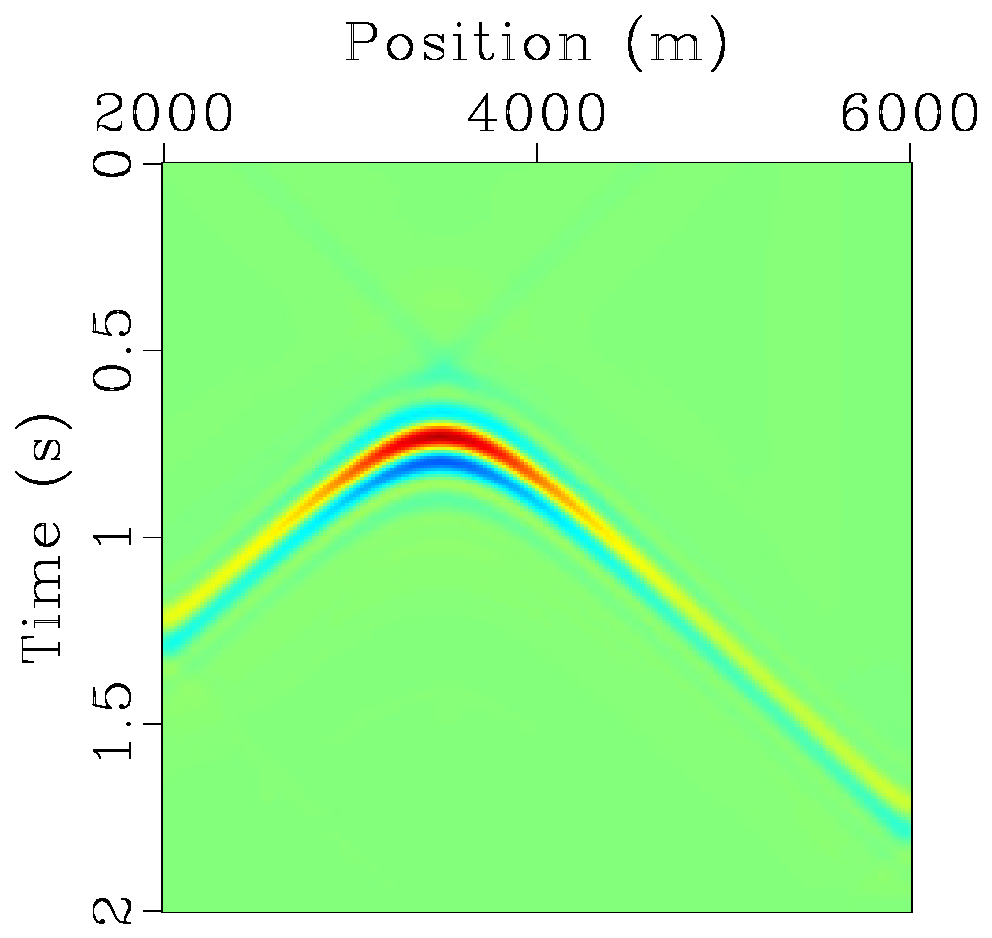
\includegraphics[width=0.45\textwidth]{preddnshshh0.pdf}}
  \subfloat[\label{fig:ddiffnshshh0}]{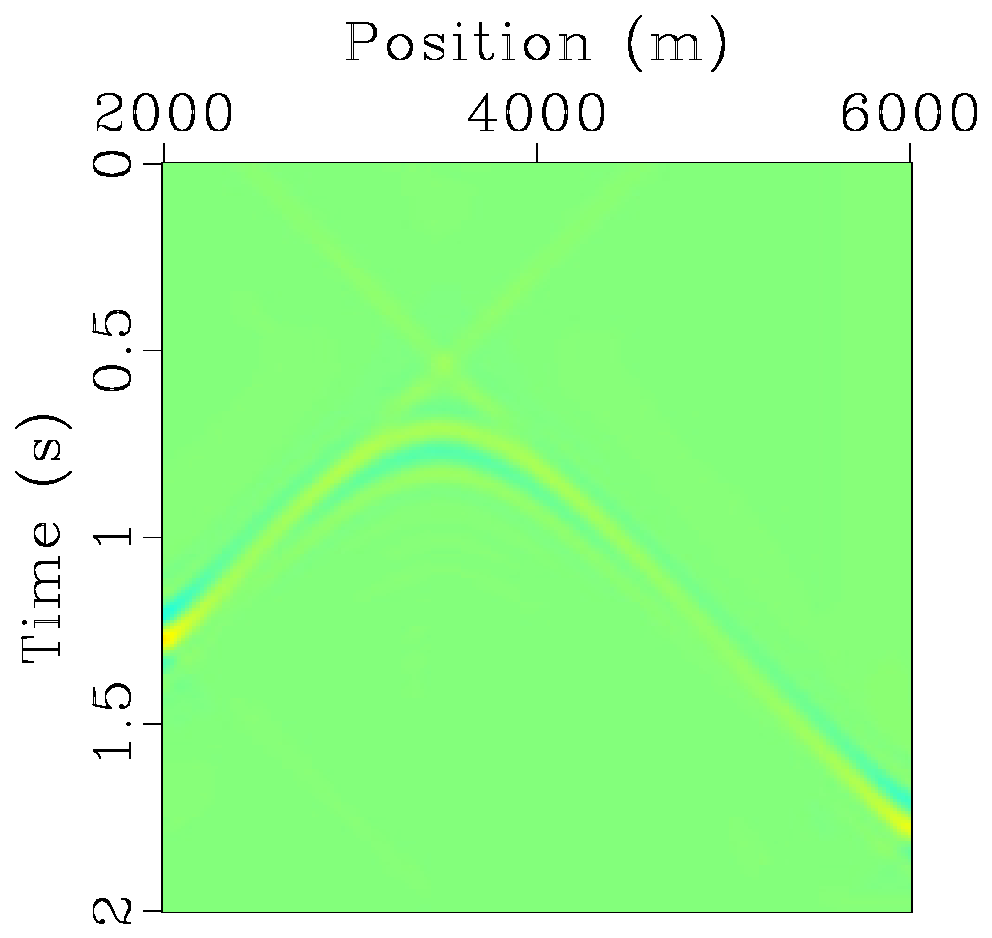
\includegraphics[width=0.45\textwidth]{ddiffnshshh0.pdf}}
  \caption{(a) Pressure source gather = image
  under pressure-to-source operator $\Lambda_s$ of pressure gather
  shown in Figure \ref{fig:dsrcphh0}, computed using
  auxiliary receiver surface``near''  at $z=2900$ m and equation \ref{eqn:lamnear}. Compare Figure
  \ref{fig:dhshh0}: because the sources and
  receivers are close, little aperture is lost in this case. (b)
  Difference between data plotted in (a)
  and source gather
  inferred from vertical velocity at source
  surface ($z=3000$ m) (Figure \ref{fig:dhshh0}). Same color scale as in Figure
  (a).}
\end{figure}

In the iterative methods to be discussed in the next section, it will
be important to be able to compute the transpose of the
pressure-to-source operator - not approximately, but to machine
precision. The prescription \ref{eqn:lamnear} only
defines an approximation. However simply substituting the right-hand
side of equation \ref{eqn:lamnear} - in effect, substituting the
approximation for the operator that it approximates - gives an
operator variant of $\Lambda_s$ with an accessible
machine-precision adjoint:
\begin{equation}
  \label{eqn:lamneartr}
 \Lambda_s^T \approx -8\Pi_1{\cal S}_a^T\Pi_0^T\Pi_1 {\cal S}_a\Pi_1^T. 
\end{equation}
From now on, when $\Lambda_s$ or $\Lambda_s^T$ appear, the symbols are
understood to mean the approximations \ref{eqn:lamnear} and
\ref{eqn:lamneartr}.

Figure \ref{fig:preddnshstrhh0} shows the image of the pressure gather
in Figure \ref{fig:dsrcphh0} under $\Lambda_s^T$ approximated as in
equation \ref{eqn:lamneartr},
using the auxiliary receiver surface at $z=2900$. Note
the close resemblance to the image of the same pressure gather under
$\Lambda_s$ displayed in Figure
\ref{fig:preddnshshh0}. The difference of these two images is
displayed in \ref{fig:ddiffnslamtrhh0}, on the same color scale as the
images themselves. Note that propagation takes place entirely in a
region where the mechanical parameters are homogenous.

\begin{figure}
  \centering
  \subfloat[\label{fig:preddnshstrhh0}]{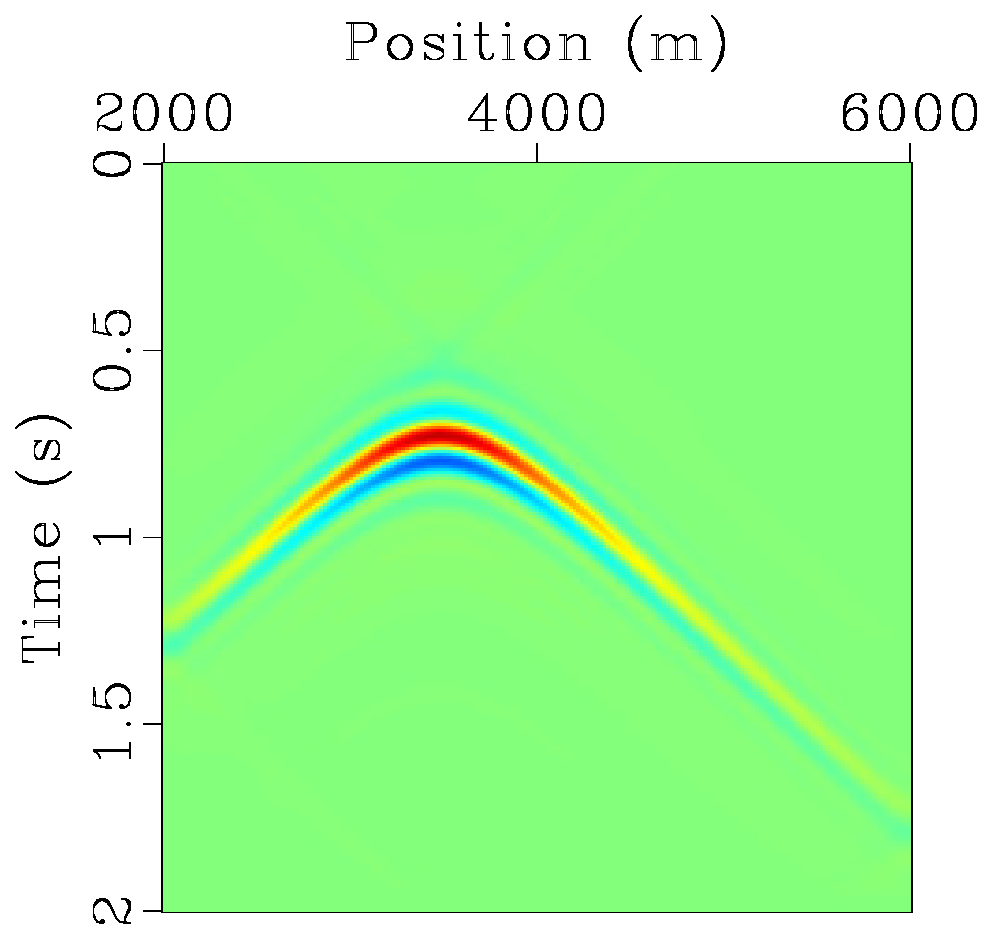
\includegraphics[width=0.45\textwidth]{preddnshstrhh0.pdf}}
  \subfloat[\label{fig:ddiffnslamtrhh0}]{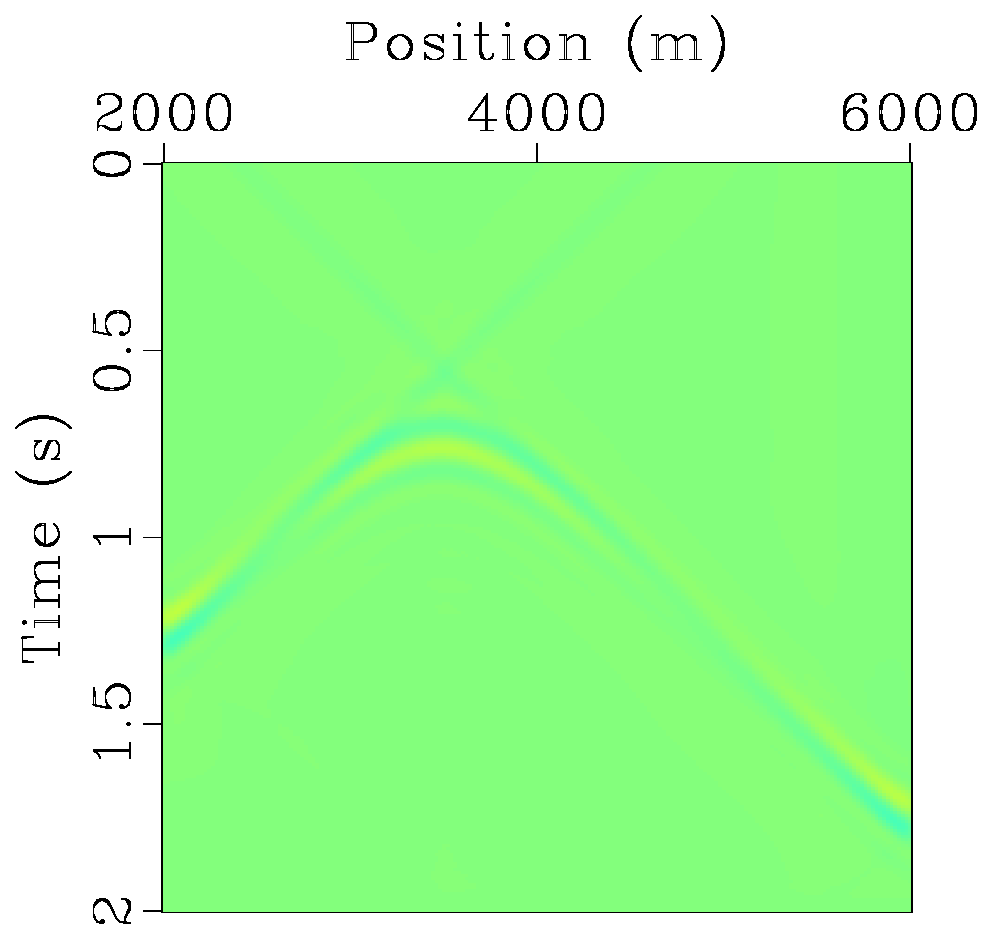
\includegraphics[width=0.45\textwidth]{ddiffnslamtrhh0.pdf}}
  \caption{(a) Pressure source gather = image
  under transposed pressure-to-source operator $\Lambda_s^T$ of pressure gather
  shown in Figure \ref{fig:dsrcphh0}, computed using
  auxiliary receiver surface``near''  at $z=2900$ m and equation \ref{eqn:lamneartr}. Compare Figure
  \ref{fig:dhshh0}: because the sources and
  receivers are close, little aperture is lost in this case. (b) Difference between (a) 
  and source gather inferred from vertical velocity at source
  surface ($z=3000$ m) (Figure \ref{fig:dhshh0}). Same color scale as (a).}
\end{figure}



\section{Accelerated Iterative Inversion}

The preceding sections provide an approximate inverse for the modeling
operator $S$ and a means to compute it effectively. These constitute
the basic ingredients of an effective preconditioning strategy. The
remaining tasks are: the construction of weighted norms making $S$
approximately unitary (insofar as possible), definition of a formal
preconditioned conjugate gradient algorithm; and modification of the
symmetrized approximate inverse to account for the presence of the
penalty term. Examples illustrate the effectiveness of the resulting
preconditioning strategy.

\subsection{Symmetrization and Weighted Norms}
Since $\Lambda_s$ approximates its transpose (equation \ref{eqn:lamappsim}), it also approximates its
 symmetrization:
\begin{equation}
  \label{eqn:lamsymm}
  \frac{1}{2}(\Lambda_s^T+\Lambda_s) \approx \Lambda_s.
\end{equation}
and similarly for $\Lambda_r$.

Define
\begin{eqnarray}
  W_m^{-1}&=& \frac{1}{2}(\Lambda_s^T+
              \Lambda_s),\nonumber \\
  W_d &=& \frac{1}{2}(\Lambda_r^T+ \Lambda_r)
          \label{eqn:wdef}
\end{eqnarray}
(the subscripts signify ``model space'' and ``data space'' of $S$).
These operators define (semi)-norms in the spaces of finite energy
pressure fields on $\Sigma_s$ and $\Sigma_r$:
\[
  \|p_s\|^2 = \langle p_s, W_m p_s\rangle,  \|p_r\|^2 = \langle p_r,
  W_d p_r\rangle,
\] 
The identification of the symmetrized $\Lambda_s$ as the inverse
of another operator $W_m$ is formal at this point, since the former operator is
likely to have null (or nearly-null) vectors due to aperture-related
amplitude loss, and certainly due to asymptotic vanishing at
non-propagating waves. Since some version of $W_m$ is essential in the
formulation for effective preconditioning, I will derive a usable
candidate to stand in for it below.

The adjoint of $S$ with respect to the weighted norms is given
approximately by
\begin{equation}
\label{eqn:wadj}
S^{\dagger} \approx  W_m^{-1}S^TW_d,
\end{equation}
As we have shown (equations \ref{eqn:baseinv}, \ref{eqn:rightinv}),
$S^{\dagger}$ is an approximate right inverse to $S$: repeating
equation \ref{eqn:rightinv} for convenience,
\begin{equation}
  \label{eqn:wunitary}
  SS^{\dagger} \approx I.
\end{equation}
This is not quite enough to establish that
$S$ is approximately unitary with respect to the
weighted norms defined by $W_m$ and $W_d$, since that would require
that $S^{\dagger}$ also be an approximate left inverse. The ray
conditions assumed throughout include the presumption that all rays
carrying high frequency energy arriving at the receiver surface
(within the support of the sampling operator) pass
over the source surface. Consequently a source supported on the source
surface exists that produces this data. However it was not assumed
that all rays passing over the source surface arrive at the receiver
surface. Therefore high frequency energy can be emitted from the
source surface without arriving at the receiver surface. We have seen
examples of this phenomenon already. The extended source shown in Figure
\ref{fig:ndwdataresrcplbulksm0} generates the diving wave data shown
in Figure \ref{fig:ndwdata0} to close approximation, even though the
latter was generated by a point source. The difference between the
extended source in Figure \ref{fig:ndwdataresrcplbulksm0} and the
point source depicted in Figure \ref{fig:ooplrays0} is an approximate
null vector for the modeling operator $S$ as defined for this
example.

In fact, that is true for the difference between $S^{\dagger}Sh$ and
$h$ for any extended source $h$:
\[
  S(S^{\dagger}Sh - h) = (SS^{\dagger}-I)Sh \approx 0.
\]
Suppose that $n$ is an approximate null vector for $S$, and $h$ is any
other extended source. Then
\[
  \langle S^{\dagger}S h, n \rangle_m = \langle Sh, Sn \rangle_d
  \approx 0.
\]
That is, $S^{\dagger}S$ is the (approximate) orthogonal projector onto
the orthocomplement of the null space of $S$. So iterations such as CG
based on $S^{\dagger}S$ construct approximation sequences lying close
to this orthocomplement, as if the null space did not exist. This
observation allows us to treat $S$ as if it were unitary in discussing
the behaviour of Krylov space algorithms based on the weighted spaces,
even though it actually is not.

Similar relations have been derived for other wave-theoretic modeling operators,
and have been used to accelerate iterative solutions of inverse
scatering problems: \cite{DafniSymes:SEG18b} review some of this
literature.

Concerning computation, just as for the pressure-to-source operators,
the weight operators are to be understood as replaced by their
approximations via equations \ref{eqn:lamnear} and \ref{eqn:lamneartr}:
\[
W_m^{-1} = \frac{1}{2}(\Lambda_s +
\Lambda_s^T)
\]
\begin{equation}
  \label{eqn:winvcomp}
  -4\Pi_1 {\cal S}_a^T(\Pi_0^T\Pi_1+ \Pi_1^T\Pi_0){\cal S}_a\Pi_0.
\end{equation}
with a similar approximate realization of $W_d$.

Figure \ref{fig:symmdnshshh0} shows the output of the symmetrized
approximate pressure-to-source operator per equation \ref{eqn:winvcomp},
applied once again to the pressure data in Figure
\ref{fig:dsrcphh0}. Note the resemblance to Figures
\ref{fig:preddnshshh0} and \ref{fig:preddnshstrhh0}. These are all
asymptotic approximations of each other. Figure
\ref{fig:ddiffsymmdnshsll0} shows the
 the difference between the pressure gather at $z=z_r$ produced from
 the pressure source output by the symmetrized $\Lambda$, and the point source
simulation (Figure \ref{fig:dfwdplh0}), plotted on the same scale as
the latter, in both cases with all propagations in the lens model.

\begin{figure}
  \centering
  \subfloat[\label{fig:symmdnshshh0}]{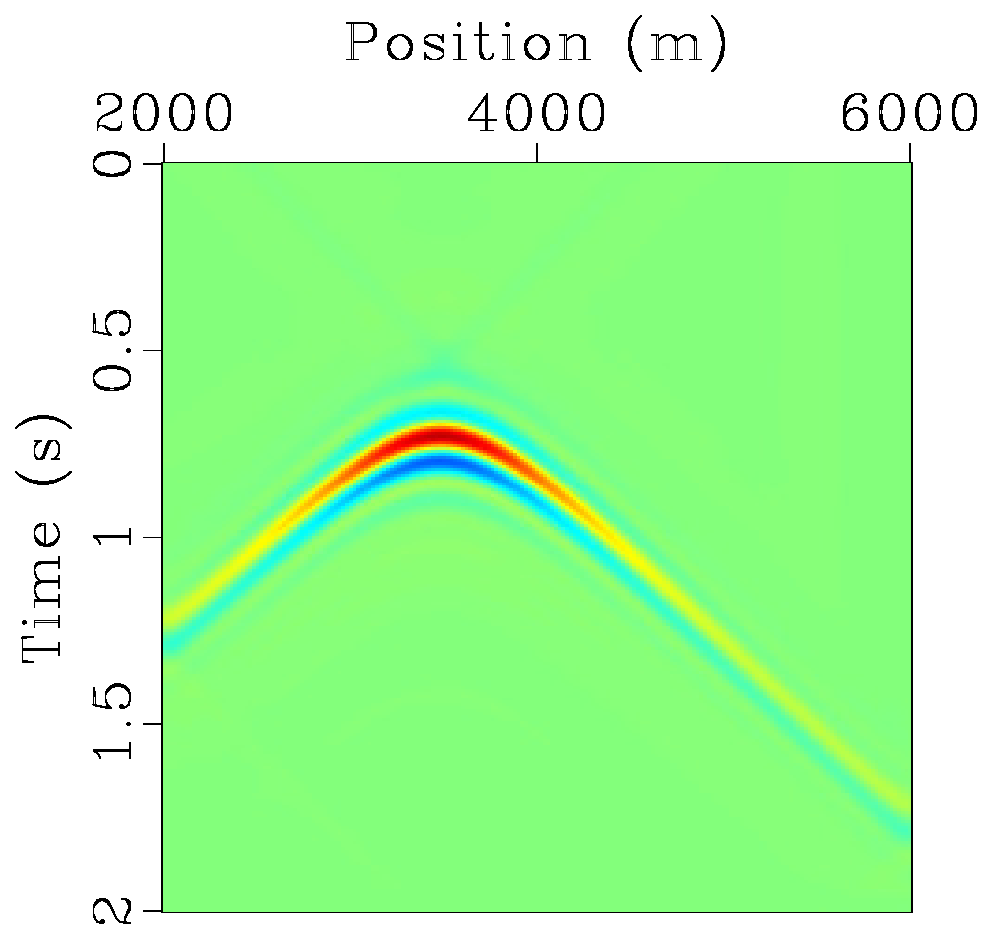
\includegraphics[width=0.45\textwidth]{symmdnshshh0.pdf}}
  \subfloat[\label{fig:ddiffsymmdnshsll0}]{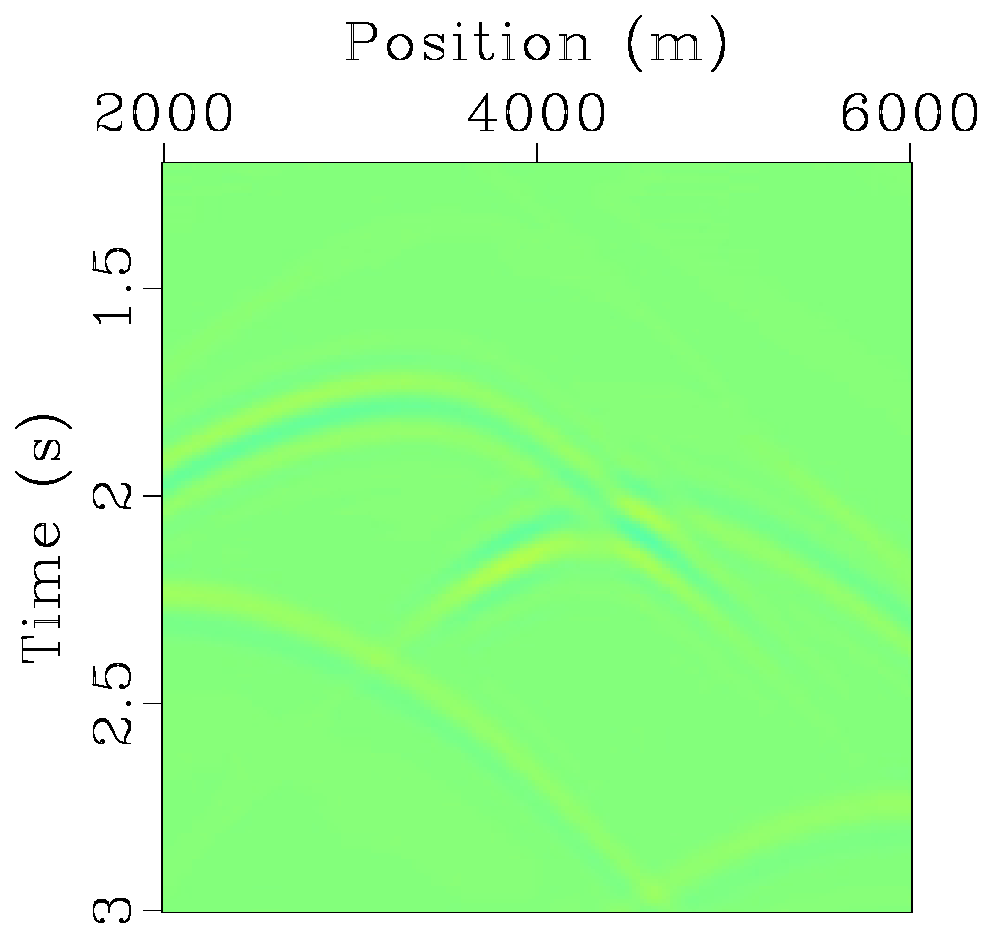
\includegraphics[width=0.45\textwidth]{ddiffsymmdnshsll0.pdf}}
  \caption{(a) Pressure source gather = image
  under symmetrized pressure-to-source operator $W_m^{-1}$ applied to pressure gather
  shown in Figure \ref{fig:dsrcphh0}, computed using
  auxiliary receiver surface``near''  at $z=2900$ m and 
  equation \ref{eqn:winvcomp}. Compare Figures
  \ref{fig:dhshh0}, \ref{fig:preddnshshh0} and
  \ref{fig:preddnshstrhh0}: these are all asymptotic approximations of
  each other. (b) Difference between pressure gather at the receiver
  surface $\Sigma_r$  ($z=1000$ m) modeled using symmetrized
  pressure-to-source gather in (a), and pressure gather shown in Figure \ref{fig:dfwdplh0},
  propagated in lens model from 
  source gather shown in Figure \ref{fig:dhshh0} (inferred from vertical velocity at source
  surface ($z=3000$ m)). Same color scale as
  Figures \ref{fig:drecplh0} and \ref{fig:dfwdplh0}.}
\end{figure}

The identity \ref{eqn:winvcomp} shows that only one forward and one adjoint simulation
are necessary to compute the action of $W_m^{-1}$ or $W_d$, and only
over the truncated computational domain between the source or receiver
surface and its auxiliary, nearby surface. The operator
in the center of the expression on the right-hand side, $\Pi_0^T\Pi_1
+ \Pi_1^T\Pi_0$, simply exchanges the components of the acoustic
fields, passing the velocity field as a pressure source and the
pressure field as a velocity source.

One more computation is required for the full implementation of the
preconditioning strategy explained in the last section: $W_m$ is
required, not just $W_m^{-1}$. Note that $W_m$ plays two roles in the
second term in equation \ref{eqn:norm1}, below: it is the weight matrix for
both the domain and range norms for $A$. It is perfectly OK for one of
these to be replaced by an asymptotic approximation, so long as it is
symmetric and computable (and at least semi-definite). Manipulations
very similar to those used to obtain equation \ref{eqn:winvcomp} lead
to the approximation
\begin{equation}
  \label{wcomp}
 W_m \approx -\frac{1}{16}\left(\Pi_0 {\cal S}_a^T
   (\Pi_1^T \Pi_0 + \Pi_0^T \Pi_1) {\cal S}_a \Pi_0^T\right)
\end{equation}
Comparison with the definition \ref{eqn:winvcomp} shows that
$W_m$ and $W_m^{-1}$ differ only in the initial and
final projection factors (and overall scale), and in particular either
can be computed for the cost of a forward/adjoint operator pair. Note
that $W_m^{-1}$ is inverse to $W_m$ only in an
approximate (asymptotic, aperture-limited) sense.

\subsection{Preconditioned Conjugate Gradient Iteration}

The most convenient arrangement the Conjugate Gradient (CG) algorithm
taking advantage of the structure \ref{eqn:wadj} is the {\em
  Preconditioned CG}. Allowing that the fit error will be measured by
the data space norm, the least squares problem to be solved is not
just $Sh \approx d$, but a regularized version:
\begin{equation}
  \label{eqn:einv}
  \mbox{minimize}_h \|Sh-d\|^2_d + \alpha^2 \|Ah\|^2_m
\end{equation}

\noindent {\bf Remark:} recall that the modified data space norm $\|d\|_d^2 = \langle
d, W_d d\rangle$ has physical meaning: for acoustics, it is
proportional to the power transmitted to the fluid by the source
corresponding to $d$. 

The minimizer of the objective defined in equation \ref{eqn:einv}
solves the normal equation
\begin{equation}
  \label{eqn:norm0}
  (S^{\dagger}S + \alpha^2 A^{\dagger}A)h = S^{\dagger}d 
\end{equation}
where the weighted adjoint $S^{\dagger}$ has already been defined in equation \ref{eqn:wadj}, and $A^{\dagger}$ is the adjoint of $A$ in the weighted model space norm defined by $W_m$, namely
\begin{equation}
  \label{eqn:aadj}
  A^{\dagger} = W_m^{-1}A^TW_m.
\end{equation}

Rewrite the normal equation \ref{eqn:norm0} as
\begin{equation}
  \label{eqn:norm1}
  W_m^{-1}(S^TW_dS + \alpha^2 A^TW_mA)h = W_m^{-1}S^TW_md 
\end{equation}
Since $W_m$ is self-adjoint and positive semidefinite, the common factor on both sides of \ref{eqn:norm1} can be re-written as
\begin{equation}
  \label{eqn:normpart}
  Nh = (S^*S + \alpha^2 A^*A)h = S^*d 
\end{equation}
in which $S^*, A^*$ are the adjoints with the original (Euclidean)
inner product in the domains but the weighted inner product in data
space:
\begin{eqnarray}
  \label{eqn:sadjwt}
  S^* &=& S^T W_d,\\
  A^* &=& A^T W_m.
\end{eqnarray}
Note the $S^*S$ and $A^*A$ are symmetric in the Euclidean sense, so
equation \ref{eqn:normpart} is a symmetric positive (semi-)definite
linear system, just the sort of thing for which the 
The Preconditioned Conjugate Gradient (``PCG'') algorithm was
designed. PCG for solution
of equation \ref{eqn:normpart} with preconditioner $M$ is usually
written as Algorithm 1 (see for example \cite{Golub:2012}):

\begin{algorithm}[H]
\caption{Preconditioned Conjugate Gradient Algorithm, Standard Version}
\begin{algorithmic}[1]
\State Choose $h_0=0$ 
  \State $r_0 \gets S^*d$
  \State $p_0 \gets M^{-1} r_0$
  \State $g_0 \gets p_0$
  \State $q_0 \gets Np_0$
  \State $k \gets 0$
  \Repeat
  \State $\alpha_k \gets \frac{\langle g_k,r_k \rangle}{\langle p_k,q_k\rangle}$
  \State $h_{k+1} \gets h_k + \alpha_k p_k$
  \State $r_{k+1} \gets r_k - \alpha_kq_k$
  \State $g_{k+1} \gets M^{-1} r_{k+1}$
  \State $\beta_{k+1} \gets \frac{\langle g_{k+1},r_{k+1}\rangle}{\langle g_k,r_k\rangle}$
  \State $p_{k+1}\gets g_{k+1}+\beta_{k+1}p_k$
  \State $q_{k+1} \gets Np_{k+1}$
  \State $k \gets k+1$
  \Until{Error is sufficiently small, or max iteration count exceeded} 
\end{algorithmic}
\end{algorithm}
The iteration converges rapidly if $M^{-1}N \approx I$. This is true
if and only if the symmetrized operator $M^{-1/2}NM^{-1/2} \approx I$,
which is in turn true if the eigenvalues of $M^{-1/2}NM^{-1/2}$ are
close to 1 (actually works well is most of these eigenvalues are close
to 1, and the rest are small - which is the case for the current
problem)..  Further, PCG is computationally effective if M is easy to
invert.

\subsection{Preconditioning with Penalty}

Note that the normal operator appearing on the left-hand side of
\ref{eqn:norm0} is not an approximate identity, due to the presence of
the regularization term: the spectrum increases in spread with
increasing $\alpha$, leading to slower convergence. We have already
observed that the pressure-to-source operators $\Lambda_s$ and
$\Lambda_r$ are pseudodifferential, and $A$ is pseudodifferential as
well. The rules for calculation of
compositions and inverses for such operators show that the operators
$W_m^{-1}$ (properly interpreted) and $W_m$ are also pseudodifferential.
Scalar pseudodifferential operators approximately
commute, so $A^{\dagger} \approx A^T$. Therefore
\begin{equation}
  \label{eqn:normapprox}
  S^{\dagger}S + \alpha^2 A^{\dagger}A \approx I + \alpha^2A^TA
\end{equation}
(restricted to the orthocomplement of the null space of $S$).
Recall that $A$ is simply multiplication by the Euclidean distance to
the physical source point $\bx_s$: $A u (\bx) = |\bx-\bx_s|u(\bx),
A^TAu(\bx) = |\bx-\bx_s|^2u(\bx)$. So the equation $(I+\alpha^2
A^TA)u=b$ is trivial to solve, and this is a key characteristic of a
good preconditioner. 


From \ref{eqn:normapprox} and \ref{eqn:norm1}, it follows that
\[
  W_m^{-1}(S^TW_dS + \alpha^2 A^TW_mA) \approx I + \alpha^2 A^TA.
\]
This observation suggests using $M=W_m(I+\alpha^2A^TA)$. This choice
is not symmetric, but since the operators on the right-hand side are
scalar pseudodifferential hence commute, it is equivalent to use of
\begin{eqnarray}
  M         &=&(I+\alpha^2A^TA)^{1/2}W_m(I+\alpha^2A^TA)^{1/2},\nonumber \\
  M^{-1}
            &=&(I+\alpha^2A^TA)^{-1/2}W_m^{-1}(I+\alpha^2A^TA)^{-1/2}.
                \label{eqn:defprecond}
\end{eqnarray}
With this choice, \ref{eqn:normapprox} implies that
$M^{-1}N \approx I$, also $M$ is symmetric. As already mentioned,
powers of $I + \alpha^2A^TA$ are trivial to compute, given the choice
of $A$ made here. 

\subsection{Example}
This final subsection shows that result of Conjugate Gradient
iteration, with and without preconditioning, applied to the source
estimation problem \ref{eqn:esis}, with zero and non-zero penalty
weight $\alpha$. The data $d$ is the gather shown in
\ref{fig:drecplh0}, simulated using the lens model (Figure \ref{fig:ooplrays0}) with source shown
in Figure \ref{fig:dsrcphh0}, or, alternatively, a point source with
bandpass filter wavelet located at $x_d=3500$ m, $z_d=3500$ m. In the inversion,
the material model is taken to be homogeneous, as has been the case in
all of the previous examples. 

Figure \ref{fig:compnres0lh0} shows the progress of the normal residual
(Euclidean norm of the difference of the two sides of equation \ref{eqn:norm1}),
for Conjugate Gradient and Preconditioned Conjugate Gradient
(Algorithm 1) iterations, applied to solution of the optimization
problem \ref{eqn:einv} with $\alpha=0$. Because the normal residual is 
measured in the Euclidean norm for both CG and PCG, the results are
comparable. For PCG, the preconditioner $M$ is given by equation
\ref{eqn:defprecond}, with the symmetrized $\Lambda$s computed as
indicated in the preceding section with auxiliary source and
receiver surfaces shifted by 100 m. Convergence for the
preconditioned algorithm is roughly 4 times as fast: this speed
comparison is much more obvious in a vertically stretched version of
the figure (Figure \ref{fig:compnrestrunc0lh0}).

%\plot{compnres0lh0}{width=\textwidth}{Comparison of normal residual 
%  (gradient) Euclidean norms: CG (blue), PCG (red), plotted 
%  vs. iteration. Data = lens model, point source (Figure 
%  \ref{fig:drecplh0}), inversion in homogenous model. Penalty weight 
%  $\alpha=0$.}

\begin{figure}
  \centering
  \subfloat[\label{fig:compnres0lh0}]{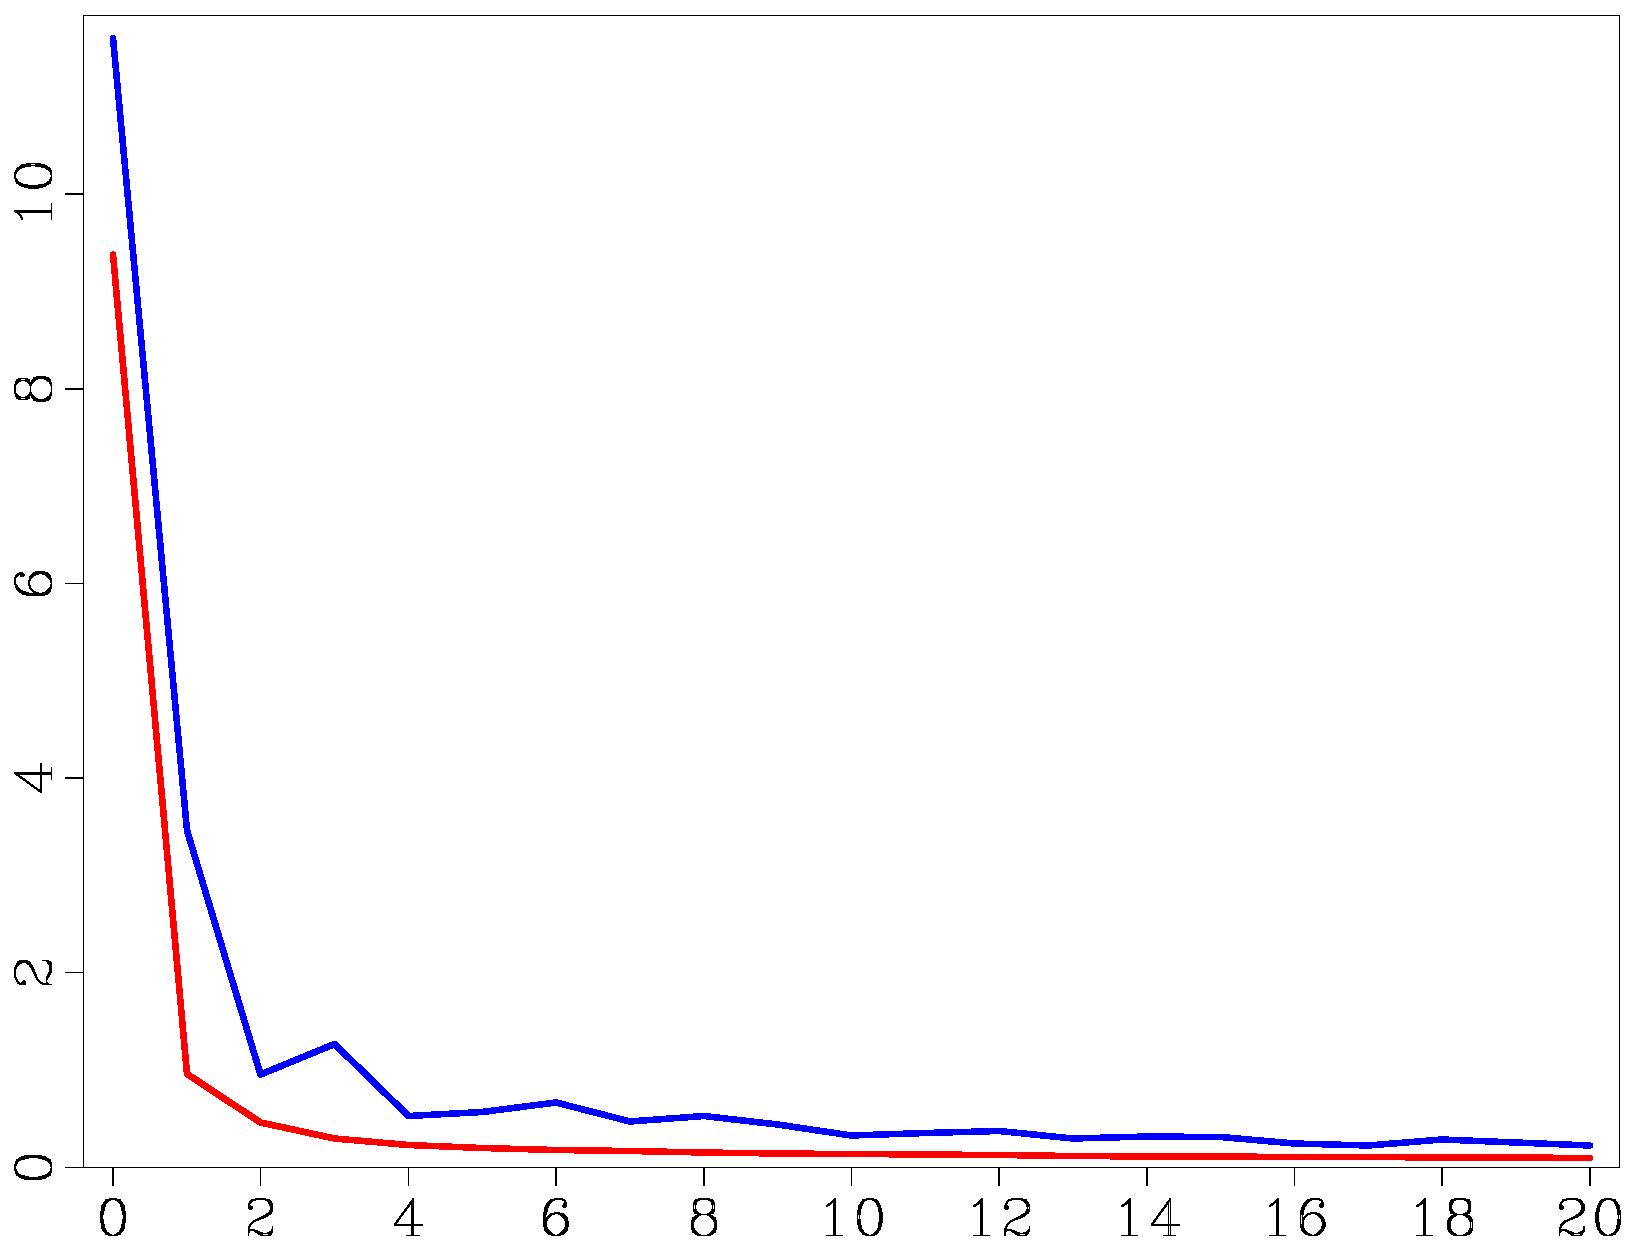
\includegraphics[width=0.45\textwidth]{compnres0lh0.pdf}}
  \subfloat[\label{fig:compnrestrunc0lh0}]{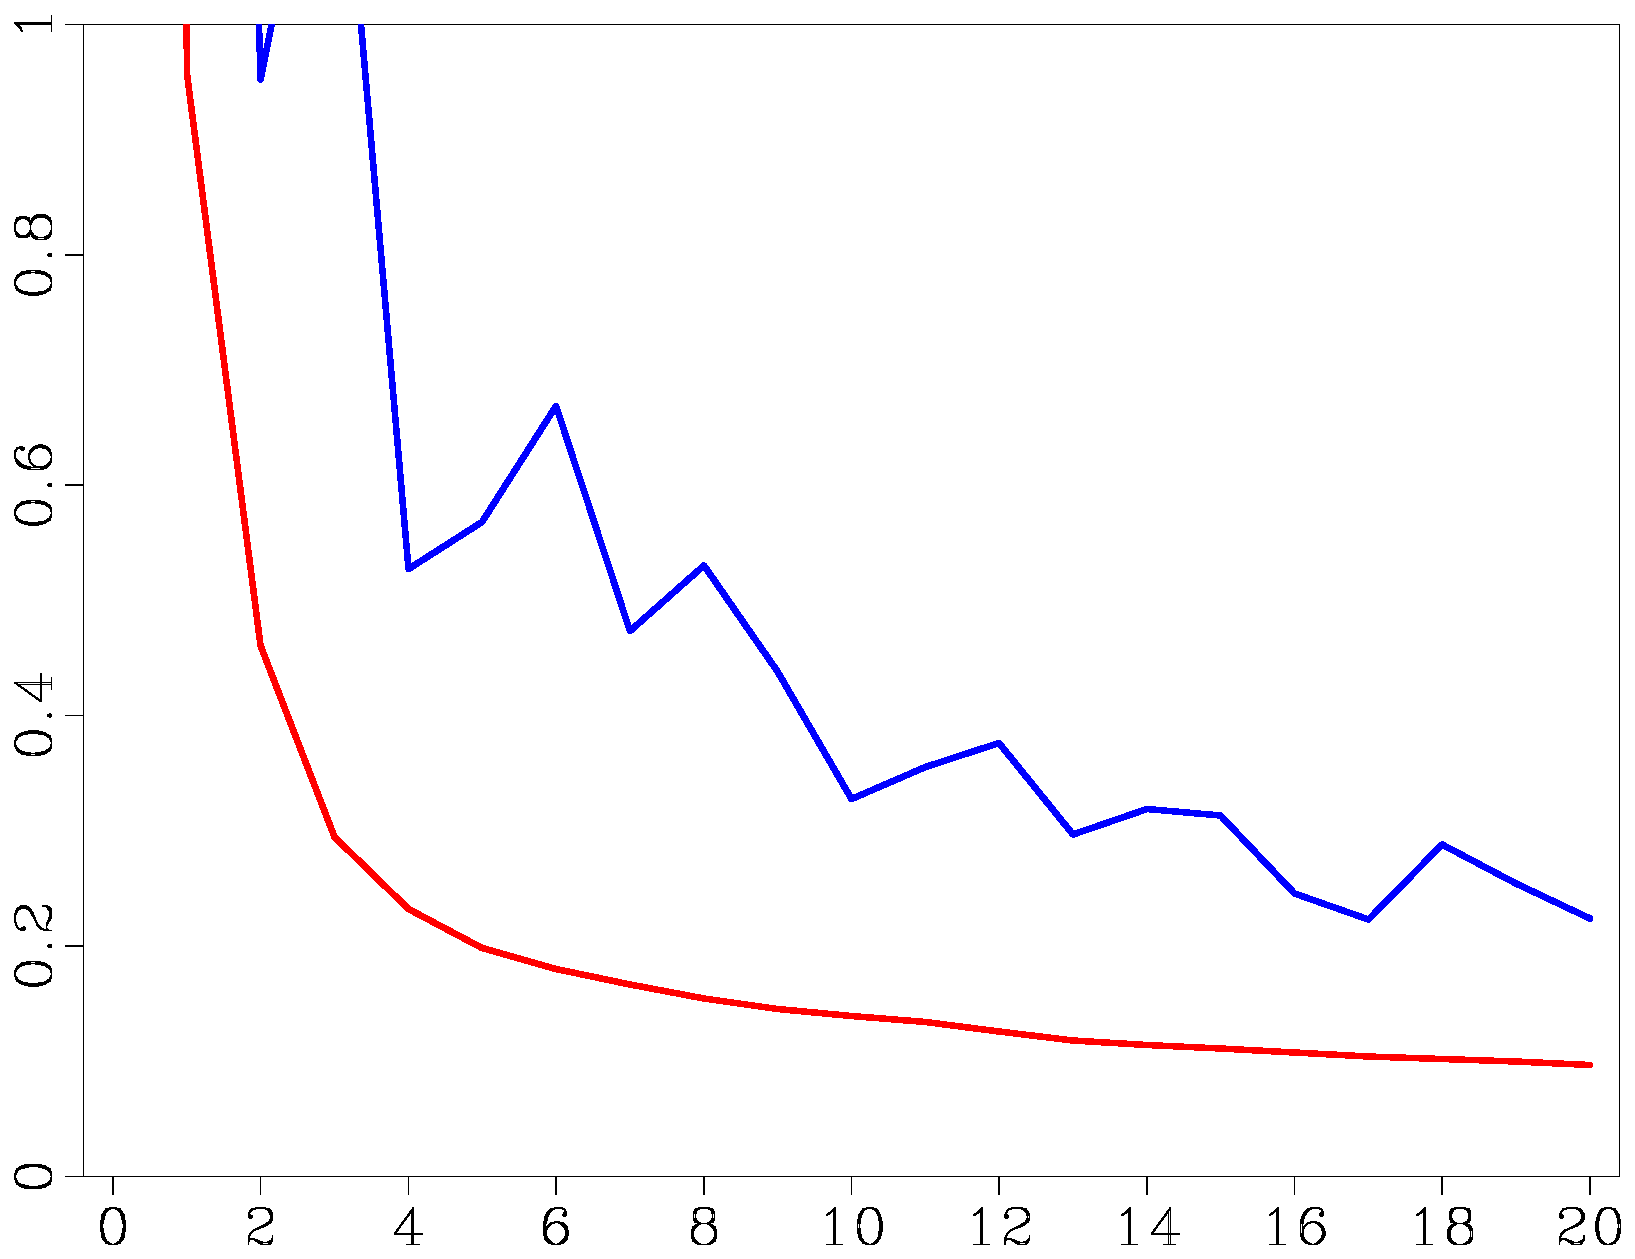
\includegraphics[width=0.45\textwidth]{compnrestrunc0lh0.pdf}}
  \caption{(a) Comparison of normal residual 
  (gradient) Euclidean norms: CG (blue), PCG (red), plotted 
  vs. iteration. Data = lens model, point source (Figure 
  \ref{fig:drecplh0}), inversion in homogenous model. Penalty weight 
  $\alpha=0$. (b) Same comparison, with expanded vertical scale, to
  show more clearly that PCG ir roughly 4-5 times as fast as (in
  achieving a given normal residual) as CG.}
\end{figure}

Figure \ref{fig:compnres1lh0} shows the same comparison with non-zero
penalty weight, $\alpha=10^{-3}$. Convergence for both CG and PCG is
somewhat slower than in the $\alpha=0$ case. However the relation is
about the same, still 4-5 times as many iterations to achieve a given
normal residual level with CG as with PCG.

\begin{figure}
  \centering
  \subfloat[\label{fig:compnres1lh0}]{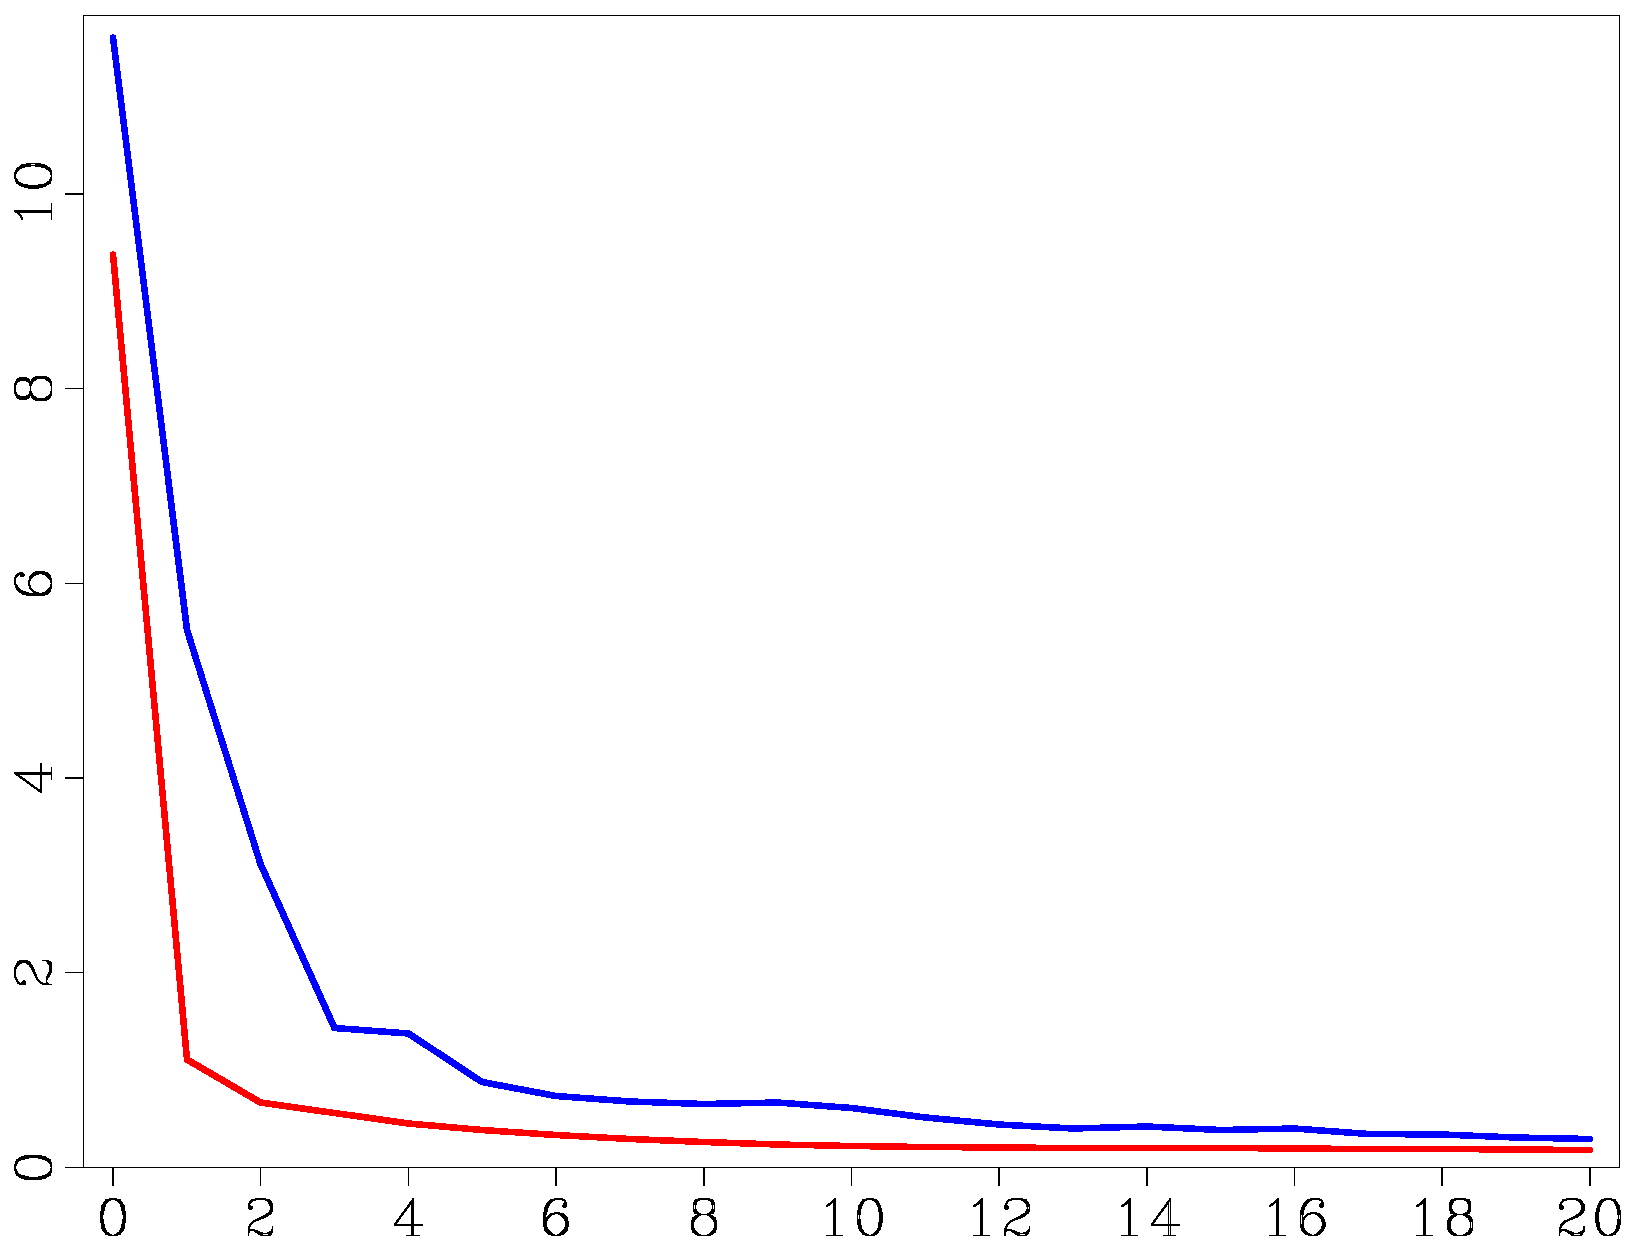
\includegraphics[width=0.45\textwidth]{compnres1lh0.pdf}}
  \subfloat[\label{fig:compnrestrunc1lh0}]{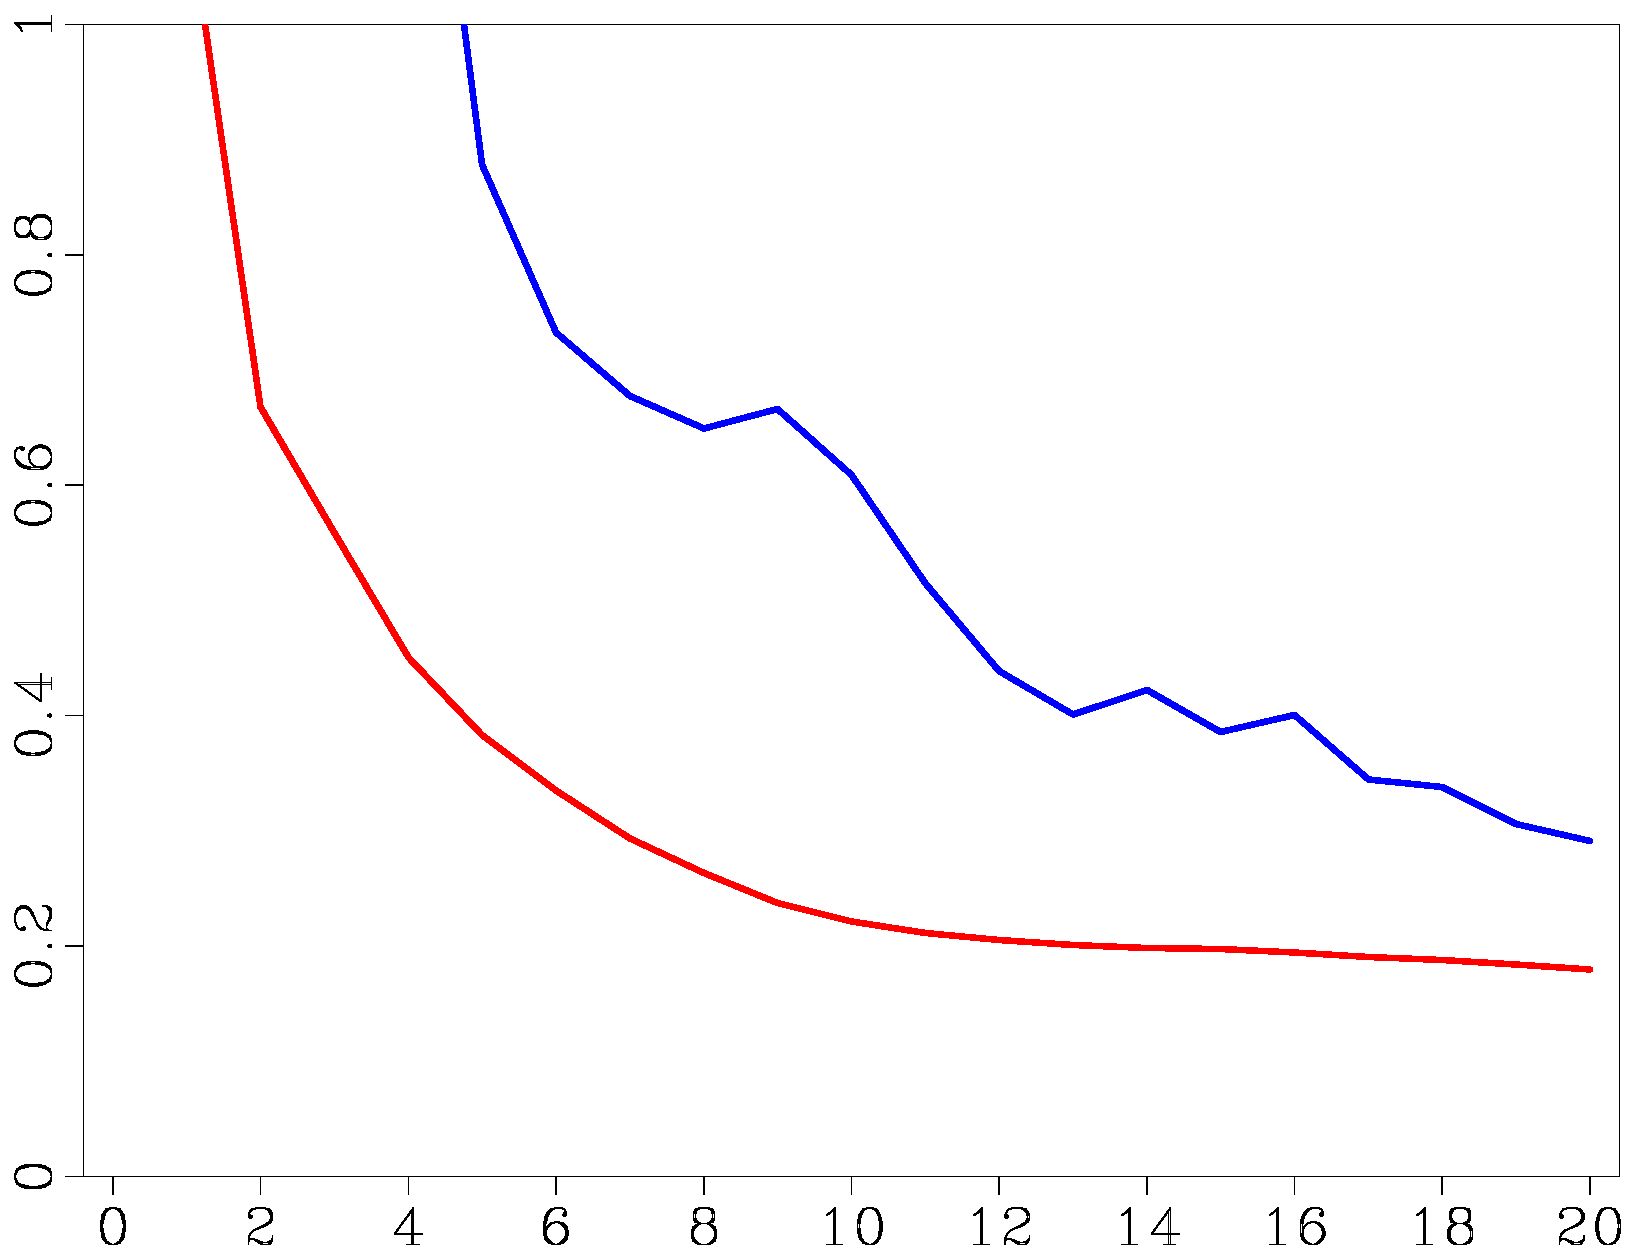
\includegraphics[width=0.45\textwidth]{compnrestrunc1lh0.pdf}}
  \caption{(a) Comparison of normal residual 
  (gradient) Euclidean norms: CG (blue), PCG (red), plotted 
  vs. iteration. Data = lens model, point source (Figure 
  \ref{fig:drecplh0}), inversion in homogenous model. Penalty weight 
  $\alpha=10^{-3}$. (b) Same comparison, with expanded vertical scale, to
  show more clearly that PCG ir roughly 4-5 times as fast as (in
  achieving a given normal residual) as CG.}
\end{figure}

%\plot{compnres1lh0}{width=\textwidth}{Comparison of normal residual 
%  (gradient) Euclidean norms: CG (blue), PCG (red), plotted 
%  vs. iteration. Data = lens model, point source (Figure 
%  \ref{fig:drecplh0}), inversion in homogenous model. Penalty weight 
%  $\alpha=10^{-3}$.}



\section{Conclusion}

The linear modeling operator of surface source extended acoustic
waveform inversion is approximately invertible, and this paper has
shown how to approximately invert it. The construction is based on
reverse time propagation of data, as inspired by the literature on
photoacoustic tomography. However, since the input energy comes from a
surface source, rather than a pressure boundary value, the
pressure-to-source operator intervenes. It provides not just an
approximate inverse, but a definition of weighted norms in domain and
range spaces of the modeling operator, in terms of which that operator
is approximately unitary. Accordingly, Krylov space iteration defined
in terms of these weighted norms, or equivalently preconditioned
Conjugate Gradient iteration, gives a rapidly convergent solution
method for the linear subproblem.

The existence of an approximate unitary representation of the modeling
operator is not merely a computational convenience, however. It
reveals fundamental aspects of the operator's structure that enable
an explanation for the mitigation of cycle-skipping, a feature of the
{\em nonlinear} extended inverse problem. This fact echoes earlier observations
concerned a reflected wave inverse problem, involving a modeling
operator with a similar approximate inverse
\cite[]{tenKroode:IPTA14,Symes:IPTA14}. Also, the approximate inverse
leads to a stable computation of the gradient of the nonlinear
objective function \ref{eqn:esi}, resolving a difficulty first noted
also for reflected wave inversion \cite[]{KerSy:94}.

All of the topics
treated here are open for elastic wave physics - the analogue of the
pressure-to-source map would is the map from surface velocity field to
corresponding constitutive defect, analogous to the elastic
Dirichlet-to-Neumann map investigated by \cite{Rachele:00}.

The underlying tool in the ideas developed here is geometric optics
(or ray theory), without which the very concept of incoming/outgoing waves
(on which these results rest) would be meaningless. The physics of actual earth materials includes
material heterogeneity on all scales, which appears to leave little
room for the assumption of scale separation underlying geometric
optics. Moreover, earth materials are anelastic, with elastic wave
energy being converted to and from thermal excitation, pore fluid
motion, and so on. A truly satisfactory understanding of inverse wave
problems will eventually need to accommodate heterogenity and
anelasticity beyond the current capabilities of the ray-based theory.

\section{Acknowledgements}
The author thanks the anonymous reviewers for their very helpful
comments and suggestions.

\section{Declarations}
\subsection{Funding}
The author did not receive support from any organization for the
submitted work.
\subsection{Competing Interests}
The author certifies that he has no affiliations with or involvement
in any organization or entity with any financial interest or
non-financial interest in the subject matter or materials discussed in
this manuscript.
\subsection{Data, Material, and Code Availability}
The computational examples reported in this work were written in the
Madagascar reproducible research framework ({\tt
  http:www.reproducibility.org}). Code and data source is available
from the author on request.


\bibliographystyle{seg}
\bibliography{../../../bib/masterref}


\end{document}
